\documentclass[conference,twocolumn]{IEEEtran}
\IEEEoverridecommandlockouts
% The preceding line is only needed to identify funding in the first footnote. If that is unneeded, please comment it out.
\usepackage{cite}
\usepackage{amsmath,amssymb,amsfonts}
\usepackage{algorithmic}
\usepackage{graphicx}
\usepackage{textcomp}
\usepackage{xcolor}
\usepackage{subcaption}

% For the tikz images
\usepackage{tikz}
\usepackage[utf8]{inputenc}
\usepackage{siunitx}
\usepackage{pgfplots}
\newcommand{\sofie}[1]{{\color{red}[sp: #1]}}
\newcommand{\achiel}[1]{{\color{green}[ac: #1]}}
\newcommand{\zh}[1]{{\color{blue}[ev: #1]}}

\newcommand\orcidicon[1]{\href{https://orcid.org/#1}{
\includegraphics[height=0.8\baselineskip]{orcid.ps}
}}


\newcommand{\orcidauthorA}{0000-0002-4156-0317}
\newcommand{\orcidauthorB}{0000-0002-1470-2076}
\newcommand{\orcidauthorC}{0000-0003-1238-2002}


\DeclareUnicodeCharacter{2212}{−}
\usepgfplotslibrary{groupplots,dateplot,polar}
\usetikzlibrary{patterns,shapes.arrows}
\pgfplotsset{compat=newest,every axis/.append style={font=\scriptsize,
                              width=\linewidth,
                              height=0.6\linewidth}}



\def\BibTeX{{\rm B\kern-.05em{\sc i\kern-.025em b}\kern-.08em
    T\kern-.1667em\lower.7ex\hbox{E}\kern-.125emX}}
\begin{document}

\title{3D beamforming and handover analysis for UAV networks\\
\thanks{This research is supported by the Research Foundation Flanders (FWO), project no. S003817N (OmniDrone) and by the European Union’s Horizon
2020 under grant agreement no. 732174 (ORCA project) .}
}

\author{\IEEEauthorblockN{
Achiel Colpaert, %\orcidicon{0000-0003-1238-2002},
Evgenii Vinogradov, %\orcidicon{0000-0002-4156-0317},
and Sofie Pollin %\orcidicon{0000-0002-1470-2076}
}
\IEEEauthorblockA{KU Leuven, ESAT - Department of Electrical Engineering, Kasteelpark Arenberg 10, 3001 Heverlee, Belgium\\
E-mail: \{achiel.colpaert, evgenii.vinogradov, sofie.pollin\}@kuleuven.be}}

\maketitle  

\begin{abstract}
In future drone applications fast moving unmanned aerial vehicles (UAVs) will need to be connected via a high throughput ultra reliable wireless link. MmWave communication is assumed to be a promising technology for UAV communication, as the narrow beams cause little interference to and from the ground. A challenge for such networks is the beamforming requirement, and the fact that frequent handovers are required as the cells are small. In the UAV communication research community, mobility and especially handovers are often neglected, however when considering beamforming, antenna array sizes start to matter and the effect of azimuth and elevation should be studied, especially their impact on handover rate and outage capacity. This paper aims to fill some of this knowledge gap and to shed some light on the existing problems. This work will analyse the performance of 3D beamforming and handovers for UAV networks through a case study of a realistic 5G deployment using mmWave. We will look at the performance of a UAV flying over a city utilizing a beamformed mmWave link. 
% We will investigate the handover situation in both a 4G deployment without beamforming and a 5G deployment with beamforming. We suggest improvements for the handover thresholds in both scenario's.
% Secondly we will investigate the effect of these handovers on the reliability of the system. Can we improve this reliability further by considering packet duplication/dual connectivity?
\end{abstract}

\begin{IEEEkeywords}
UAV, mmWave, 5G NR, handovers, beamforming, mobility, beamtracking, antenna pattern, outage
\end{IEEEkeywords}

\section{Introduction}
\subsection{Background}
\par Drones are becoming more and more ubiquitous in our daily life. Several industries are looking at drones to improve or create new services. In these new applications unmanned aerial vehicle (UAVs) often operate in a beyond-line-of-sight manner and to control these applications a reliable wireless link is required albeit with limited capacity. However, some companies have expressed their interest in streaming high definition (HD) video over a wireless link from a drone requiring both a high throughput and reliable link.
\par Serving UAVs in beyond-line-of-sight operation by using the existing cellular network is the next logical step. Cellular networks provide omnipresent coverage and they should support the requirements for command-and-control and even high throughput links. The 3GPP initiative has even taken the first steps towards incorporating UAV users into their future standards by publishing technical report on this topic \cite{3gpp.36.777}.
\subsection{State of the art}
\par While these cellular networks sound promising, research has indicated that introducing drones into cellular networks will create several problems. First of all, authors of \cite{ Colpaert2018, Azari2018} show using either stochastic or semi-deterministic simulations that aerial users experience mainly line-of-sight (LOS) propagation conditions to multiple basestations (BS). While this is an advantage when considering the signal of the serving BS, it has been proven problematic in terms of interference caused by neighbouring BSs. They show that UAVs operate mainly in the interference limited domain instead of the usual noise limited domain for ground users. Other works have confirmed these results by performing outdoor experiments \cite{QualcommTechnologies2017, VanDerBergh2016}. The first found that the link quality at several altitudes should be sufficient to support command-and-control operation, although they mainly performed measurements in a semi-urban, close to rural, environment \cite{QualcommTechnologies2017}. The second showed through measurements at larger altitudes that the number of BSs causing interference rises dramatically when the UAV rises in altitude \cite{VanDerBergh2016}. 
\par Another problem introduced by aerial users is the interference generated in the uplink to other BSs \cite{VanDerBergh2016}, as well as the interference to to other ground applications such as satellite ground stations \cite{Vinogradov2019}. This last work suggests some interference countering techniques such as simply defining no-fly zones, more advanced antennas on the UAV side or the use of beamsteering.
\par Several solutions have already been proposed to solve these interference issues. Optimizing the cellular network configurations has been suggested by \cite{Azari2019}, such as optimizing the BS antenna tilt, however we cannot assume that providers will sacrifice performance for ground users in order to support aerial users. Several works suggest that directive antennas and beamforming will allow the BS to spatially separate users in 3D space allowing for efficient serving of both ground and aerial users. In this context, researchers mention that 5G is a good candidate as it supports beamforming and high throughput links, while being highly configurable \cite{Lin2018}. On the other side, authors of \cite{Izydorczyk2020} suggest to put highly directive antennas on the UAV. Another solution is proposed by the authors of \cite{Garcia-Rodriguez2019}. They suggest to use the massive MIMO support in 5G which allows the BS to not only spatially separate the the users but also create nulls at other users to further reduce the interference. In previous work, we proposed mmWave communications as a promising technology for drones as they experience mainly LOS propagation, which is a mayor requirement for mmWave communications to work \cite{Colpaert2018}. The larger pathloss at mmWave frequencies would result in less inter-cell interference, while the small antenna aperture size allows for the use of large number of antennas in an antenna array. These large antenna arrays are ideal to perform beamforming to compensate for the large pathloss at the user while simultaneously reducing interference. The use of mmWaves opens a wide spectrum to use and the high throughput mentioned earlier can be easily achieved by utilizing massive bandwidth. 
\par Previously mentioned research considered mainly static users, however, when mobile scenarios are considered even more problems arise. First of all, beam training and tracking becomes more difficult and generates a lot of overhead, however, this overhead is less than initially thought in research and thus should be able to support mobile users up to decent speeds \cite{Huang2020}. Another problem with using mmWaves is large Doppler frequency shifts as these are proportional to the center frequency. Authors of \cite{Stanczak2018} summarize several problems that arise for mobile aerial users. Aerial users are most of the time served by sidelobes of the antenna pattern in current static cellular deployments. This results in a fragmented association pattern. This fragmented association in combination with the low signal-to-interference-noise-ratio (SINR) results in a higher probability of radio link failures as well as handover failures. Due to the fragmented association pattern more ping-pong handovers will take place, where a user is handed over back to its original cell within a certain time frame. While LTE is designed to support users traveling at speeds up to 350~km/h\cite{3gpp.36.101} it assumes large cell areas and not these sidelobe based cell association patterns that UAV's experience. The 3GPP study item has identified cell selection, handover efficiency and robustness as a key performance indicators for aerial users in cellular networks\cite{3gpp.36.777}.
\par Euler et al. \cite{Euler2019} investigate this problem further on a simulation basis and they point at two problems. First, they conclude that high interference levels will make it difficult to maintain connection as well as perform successful handovers, which will lead to a large number of both radio link failures as well as handover failures.They explore is the usage of LTE-M which allows users to operate in low SINR conditions. They were able to significantly reduce the number of radio link failures and handover failures with only a slight increase in ping-pong handovers.
Secondly, they conclude that when aerial users move through antenna pattern nulls the default handover mechanism will be too slow to prevent radio link failure. To solve this issue, they suggest to tune the parameters of the handover procedure such as the reaction time.
\par With the deployment of 5G networks, \cite{Muzaffar2020} performed some preliminary experiments with a drone connected to a 5G BS at sub-6~GHz frequency. They concluded that the UAV experienced more handovers than a ground user but also that handovers to the 4G network occurred regularly reducing the overall throughput, but this will be solved by the deployment of more 5G BSs.
\par Aside from previous mentioned research, handover problems are largely neglected in the UAV research community when investigating cellular connected UAVs, especially in the context of beamforming. In the same trend, the effect of the used antenna array topology when performing beamforming is also largely disregarded in UAV studies, while in our opinion the antenna topologies can have a big influence on the behaviour of beamsteering and handovers alike.
\subsection{Problem statement}
\par In this work, we fill some of this knowledge gap regarding the effect of antenna topologies and the effect of beamforming on handover problems. This work poses as a stepping stone in the path towards the design of optimal beamforming networks for UAV communications. Regarding the antenna array topology, we investigate the effect using different topologies of different sizes and their effect on the handover behaviour and outage cost. Especially in the context of mmWaves, where a single antenna element has a physical size in the order of magnitude of millimeters, hence large number of mmWave antennas can be manufactured in a physically small antenna array \cite{Rappaport2013, Colpaert2020}. These large number of antennas allow us to create large antenna gains through beamforming, however, at the same time when using beamforming with large antenna arrays, the beamwidth becomes more and more narrow with increasing array size. One can see that at a certain point the difficulty of tracking the user with a beam as wide as a pencil will counter the gains won of using more antenna elements. Initial access will  pose problems in terms of beam discovery, although several tricks can be applied where initially wider beams are used to locate the user. When introducing user mobility even more problems arise. Keeping track of the user device with almost no margin for error proves a difficult task, especially if this user device is a UAV or any other device that needs a reliable connection to the network and is moving at larger speed than walking speed. 
\subsection{Contributions}
\par This work will show the main issues that arise when a UAV is flying over a semi-urban area while being served by 5G mmWave BSs on the ground. We will look at the handover problems and the effect of beam misalignment and how choosing the correct antenna topology could counter these problems. The main contributions of this work can be listed as follows:
\begin{itemize}
    \item Provide insight in the effect of increasing the number of antenna elements on the beamwidth and the outage probability at the UAV side;
    \item Stress the importance of highly accurate beamtracking with increasing size of the antenna arrays;
    \item Show that the UAV operating altitude should be considered when designing the antenna array on BS side;
    \item Indicate the effect of choosing different antenna array topologies on the number of handovers experienced by a UAV.
\end{itemize}
The rest of this paper is organized as follows. First, we shortly discuss the simulator environment used to simulate the behaviour of the UAVs and the network. Followed by the additions implemented to support the necessary beamforming and handovers techniques for the scenarios. Next we discuss the investigated scenarios and the parameters used. Then, we show and discuss the results and, lastly, we conclude our work. 
% \sofie{or add a figure where you show the problem statement/contributions clearly to make it more clear what the focus of the paper is?}

\section{Methods}
\par To simulate the behaviour of the UAV flying over the city we use the coverage simulator described in \cite{Colpaert2018}.
It applies the 3GPP wireless channel models \cite{3gpp.38.901} in a 3D environment to determine the received signal strength at the users. We assume a 5G deployment where a current internet service provider's (ISP's) deployment sites are equipped with 5G mmWave capabilities without adding extra locations. The location considered is the city of Leuven in Belgium and the BS deployment of a local ISP is used, where each BS has either three or four sectors each. The considered area can be seen in Figure~\ref{fig:area}. 
%The x and y-axis represent Lambert coordinates which is a localisation system used within Belgium where one pixel represents one square meter \cite{lambert}.
\begin{figure}[tbp]
\centering
% \centerline{
% \includegraphics{handover_per_min}
% }
% This file was created by tikzplotlib v0.9.3.
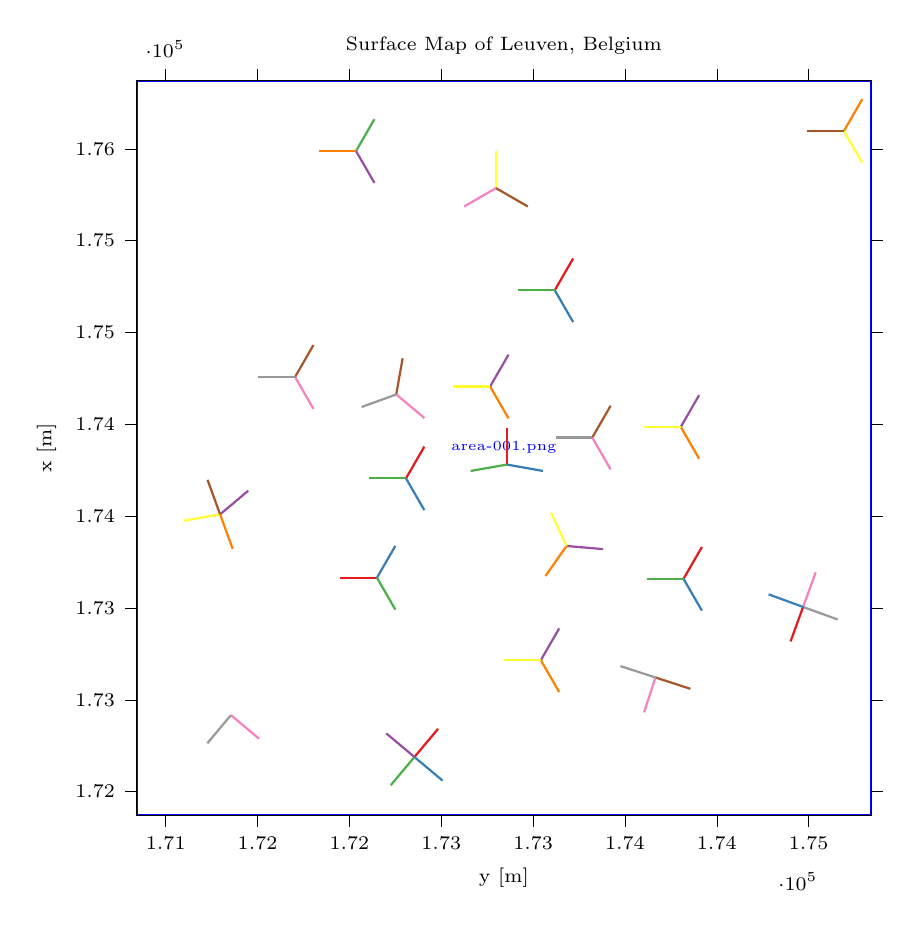
\begin{tikzpicture}

\definecolor{color0}{rgb}{0.894117647058824,0.101960784313725,0.109803921568627}
\definecolor{color1}{rgb}{0.215686274509804,0.494117647058824,0.72156862745098}
\definecolor{color2}{rgb}{0.301960784313725,0.686274509803922,0.290196078431373}
\definecolor{color3}{rgb}{0.596078431372549,0.305882352941176,0.63921568627451}
\definecolor{color4}{rgb}{1,0.498039215686275,0}
\definecolor{color5}{rgb}{1,1,0.2}
\definecolor{color6}{rgb}{0.650980392156863,0.337254901960784,0.156862745098039}
\definecolor{color7}{rgb}{0.968627450980392,0.505882352941176,0.749019607843137}

\begin{axis}[
% colorbar,
% colorbar style={ylabel={}},
% colormap/viridis,
point meta max=123,
point meta min=11.2734375,
tick align=outside,
tick pos=both,
title={Surface Map of Leuven, Belgium},
x grid style={white!69.0196078431373!black},
xmin=171341, xmax=175341,
xtick style={color=black},
y grid style={white!69.0196078431373!black},
ymin=172372, ymax=176372,
ytick style={color=black},
xlabel={y [m]},
ylabel={x [m]},
height=0.9\linewidth,
width=0.9\linewidth
]
\addplot graphics [includegraphics cmd=\pgfimage,xmin=171341, xmax=175341, ymin=172372, ymax=176372] {area-001.png};
\addplot [thick, color0]
table {%
172650 173665
172450 173665
};
\addplot [thick, color1]
table {%
172650 173665
172750 173838.205080757
};
\addplot [thick, color2]
table {%
172650 173665
172750 173491.794919243
};
\addplot [thick, color3]
table {%
173266 174706
173366 174879.205080757
};
\addplot [thick, color4]
table {%
173266 174706
173366 174532.794919243
};
\addplot [thick, color5]
table {%
173266 174706
173066 174706
};
\addplot [thick, color6]
table {%
173822 174428
173922 174601.205080757
};
\addplot [thick, color7]
table {%
173822 174428
173922 174254.794919243
};
\addplot [thick, white!60!black]
table {%
173822 174428
173622 174428
};
\addplot [thick, color0]
table {%
173618 175230
173718 175403.205080757
};
\addplot [thick, color1]
table {%
173618 175230
173718 175056.794919243
};
\addplot [thick, color2]
table {%
173618 175230
173418 175230
};
\addplot [thick, color3]
table {%
174304 174486
174404 174659.205080757
};
\addplot [thick, color4]
table {%
174304 174486
174404 174312.794919243
};
\addplot [thick, color5]
table {%
174304 174486
174104 174486
};
\addplot [thick, color6]
table {%
172204 174758
172304 174931.205080757
};
\addplot [thick, color7]
table {%
172204 174758
172304 174584.794919243
};
\addplot [thick, white!60!black]
table {%
172204 174758
172004 174758
};
\addplot [thick, color0]
table {%
172808 174206
172908 174379.205080757
};
\addplot [thick, color1]
table {%
172808 174206
172908 174032.794919243
};
\addplot [thick, color2]
table {%
172808 174206
172608 174206
};
\addplot [thick, color3]
table {%
173682 173838
173881.238939618 173820.56885145
};
\addplot [thick, color4]
table {%
173682 173838
173567.28471273 173674.169591142
};
\addplot [thick, color5]
table {%
173682 173838
173597.476347652 174019.261557407
};
\addplot [thick, color6]
table {%
172755 174663
172789.729635533 174859.961550602
};
\addplot [thick, color7]
table {%
172755 174663
172908.208888624 174534.442478063
};
\addplot [thick, white!60!black]
table {%
172755 174663
172567.061475843 174594.595971335
};
\addplot [thick, color0]
table {%
173357 174281
173357 174481
};
\addplot [thick, color1]
table {%
173357 174281
173553.961550602 174246.270364467
};
\addplot [thick, color2]
table {%
173357 174281
173160.038449398 174246.270364467
};
\addplot [thick, color3]
table {%
173542 173216
173642 173389.205080757
};
\addplot [thick, color4]
table {%
173542 173216
173642 173042.794919243
};
\addplot [thick, color5]
table {%
173542 173216
173342 173216
};
\addplot [thick, color6]
table {%
174166 173122
174356.211303259 173060.196601125
};
\addplot [thick, color7]
table {%
174166 173122
174104.196601125 172931.788696741
};
\addplot [thick, white!60!black]
table {%
174166 173122
173975.788696741 173183.803398875
};
\addplot [thick, color0]
table {%
174319 173659
174419 173832.205080757
};
\addplot [thick, color1]
table {%
174319 173659
174419 173485.794919243
};
\addplot [thick, color2]
table {%
174319 173659
174119 173659
};
\addplot [thick, color3]
table {%
171796 174010
171949.208888624 174138.557521937
};
\addplot [thick, color4]
table {%
171796 174010
171864.404028665 173822.061475843
};
\addplot [thick, color5]
table {%
171796 174010
171599.038449398 173975.270364467
};
\addplot [thick, color6]
table {%
171796 174010
171727.595971335 174197.938524157
};
\addplot [thick, color7]
table {%
171855 172917
172008.208888624 172788.442478063
};
\addplot [thick, white!60!black]
table {%
171855 172917
171726.442478063 172763.791111376
};
\addplot [thick, color0]
table {%
172854 172689
172982.557521937 172842.208888624
};
\addplot [thick, color1]
table {%
172854 172689
173007.208888624 172560.442478063
};
\addplot [thick, color2]
table {%
172854 172689
172725.442478063 172535.791111376
};
\addplot [thick, color3]
table {%
172854 172689
172700.791111376 172817.557521937
};
\addplot [thick, color4]
table {%
175192 176097
175292 176270.205080757
};
\addplot [thick, color5]
table {%
175192 176097
175292 175923.794919243
};
\addplot [thick, color6]
table {%
175192 176097
174992 176097
};
\addplot [thick, color7]
table {%
174970 173506
175038.404028665 173693.938524157
};
\addplot [thick, white!60!black]
table {%
174970 173506
175157.938524157 173437.595971335
};
\addplot [thick, color0]
table {%
174970 173506
174901.595971335 173318.061475843
};
\addplot [thick, color1]
table {%
174970 173506
174782.061475843 173574.404028665
};
\addplot [thick, color2]
table {%
172536 175988
172636 176161.205080757
};
\addplot [thick, color3]
table {%
172536 175988
172636 175814.794919243
};
\addplot [thick, color4]
table {%
172536 175988
172336 175988
};
\addplot [thick, color5]
table {%
173298 175786
173298 175986
};
\addplot [thick, color6]
table {%
173298 175786
173471.205080757 175686
};
\addplot [thick, color7]
table {%
173298 175786
173124.794919243 175686
};
\end{axis}

\end{tikzpicture}

\caption{Representation of the considered area where each pixel represents the altitude above sea-level. All BS locations are indicated with their respective sectors and orientation.}
\label{fig:area}
\end{figure}
In terms of a mmWave deployment this should be a sub-optimal configuration for ground users and further cell densification is necessary to provide decent city-wide coverage. However, for UAVs, this poses less of a problem as UAVs experience almost always LOS connections to their serving BSs, which is the ideal case for a mmWave connection.
\subsection{Beamforming and handover simulations}
Two new features have been introduced in previously mentioned simulator. First of all, support for antenna radiation patterns of antenna arrays is implemented, including the use of steering vectors. This allows for advanced beamforming and beamtracking simulations. For the single element of the array, the patch antenna pattern is used as defined in \cite{3gpp.38.901}. To simulate the exact antenna array pattern, we use the array factor defined in antenna theory. The antenna array gain in a direction is defined in \cite{Balanis2016} as $G(\theta,\phi) = G_0(\theta,\phi) * AF,$ where $\theta$ represents the elevation angle measured from the z-axis which is defined as the zenith, $\phi$ is the azimuth angle in the horizontal plane with north defined as 0 degrees, $G_0(\theta,\phi)$ the single element gain in given direction and where $AF$ represents the array factor defined as $AF = S_{z_M} \cdot S_{y_N}$,
% \begin{equation}
%     AF = S_{z_M} \cdot S_{y_N},
% \end{equation}
where:
\begin{equation}
    S_{z_M} = \sum_{m = 1}^{M}I_{m1}e^{j(m-1)(kd_zcos(\theta)+\beta_z)}
\end{equation}
\begin{equation}
    S_{y_N} = \sum_{n = 1}^{N}I_{1n}e^{j(n-1)(kd_ysin(\theta)sin(\phi)+\beta_y)},
\end{equation}
where $M$ and $N$ represent the number of antenna elements on the z and y-axis of the array, respectively, $k$ is the wave number, $d_z$ and $d_y$ are the distances between the elements on z and y-axis respectively and where $\beta_z$ and $\beta_y$ represent the factors introduced by the steering directions and they can be calculated as follows:
\begin{equation}
\beta_z = -kd_zcos(\theta_0)
\end{equation}
\begin{equation}
\beta_y = -kd_ysin(\theta_0)sin(\phi_0)
\end{equation}
where $\theta_0$ and $\phi_0$ represent the desired beamsteering direction. When discussing different array topologies we will always mention two numbers, the first being the number of antenna elements in the vertical domain $M$ and the second being the number of elements in the horizontal domain $N$. To achieve %an apples-to-apples
a fair comparison, we keep the number of antenna elements constant when comparing different antenna array shapes
%, eg. 1 by 256 compared to 128 by 2.
\par %A second new addition to the simulator are mobile users. 
Since in this paper, we aim to investigate the beam tracking effect on handovers, we have added mobility support to our simulator. While previously all users were static and snapshots in time were taken and processed, now users can move around in space and their parameters can be simultaneously monitored. Next to this mobility, a basic messaging framework was implemented to support handovers. In this framework, a user will monitor its A3 event such as defined in the 5G standard \cite{3gpp.38.331}. This event triggers when a neighbouring cell signal becomes stronger than the serving cell with a certain threshold. The threshold for this event is the A3 threshold ($T_{A3}$) and is defined in Table \ref{tab:parameters}. When the event requirements are met, the user reports basic measurements to its serving BS which in its turn will decide whether a handover needs to happen. When a handover is triggered, the user gets assigned to the desired BS and the beam of that BS is properly aligned to the user. Perfect beam alignment is always assumed and achieved at zero cost. To make the simulation more realistic, it is assumed that beams are tracked and updated as function of mobility with varying update rates as will be explained later. 
\subsection{Scenarios}
\par We consider a case study where a UAV is flying at a fixed speed of $14$~m/s (approx. $50$~km/h) with a fixed altitude above the city of Leuven. A set of random trajectories is generated where the UAV flies in a straight horizontal line in a random direction at two different altitudes of $40$~m and $150$~m. The same set of trajectories is used for every different set of parameters, this allows for a one-to-one comparison of the results. The baseline is the static scenario, where no beamtracking is enabled and where each sector antenna array is fixed towards its azimuth angle, tilted towards the ground at an angle of $7$ degrees. A X by 2 antenna array is used, with X adapted to the total number of antennas.
\par To show the impact of perfect beam alignment, we introduce some error in the alignment. The BS only periodically updates its beam alignment, which results in the serving beam not always being perfectly aligned. In the simulator, an update period of $0.1$~s is a realtime update period as the time step of the simulator is equal to $0.1$~s. The two antenna array sizes being compared are a 64-element array and a 256-element array. When comparing arrays of different sizes, square array configurations are considered. Different antenna array topologies are investigated for a 64-element and a 256-element antenna array.
\par To investigate the performance of different scenarios and topologies, we will look at the outage cost, which represents the fraction of the total travel time where the Signal-to-Noise (SNR) ratio is below the threshold of $-6$~dB, which is the minimum SNR required to provide a command-and-control link \cite{Colpaert2018}. An outage cost of one means the complete trajectory had an SNR lower than the threshold. Another performance parameter considered are the number of handovers per minute experienced. Expressing the handovers in this manner gives a good insight in the severity of this handover problem. All previously mentioned simulation parameters can be found in Table~\ref{tab:parameters}.

\begin{table}[bp]
\caption{Simulation parameters}
\begin{center}
\begin{tabular}{|c|c|}
\hline
\textbf{Parameter} & \textbf{Value}       \\
\hline
\hline
UAV heights, $h$       & $40$~m, $150$~m   \\
center frequency, $f$       & $26$ GHz      \\
signal bandwidth, $B$       & $400$ MHz      \\
transmit power, $p_{tx}$    & $18$ dB       \\
antenna element max gain, $G_0$ & $8$~dBi\\
antenna element 3dB beamwidth & 65~deg \\
noise density, $N_0$          & $-174$ dBm/Hz        \\
noise figure, $F$               & $9$ dB         \\
outage treshold & $-6$~dB \\
A3 treshold, $T_{A3}$ & $3$~dB\\ 
update periods & $0.1$~s,$0.2$~s,$0.5$~s\\
total number BSs & 20\\
total number sectors & 62\\
map area&$16~km^2$\\
number of trajectories        & $200$ \\
\hline
\end{tabular}
\label{tab:parameters}
\end{center}
\end{table}

\section{Results}
\par First we shed some light on the effect of increasing the number of antenna elements in an array on the width of the beam when performing beamforming. We consider an array of 64 antenna elements and an array of 256 antenna elements, both in a square shape. The maximum gain of these antenna arrays are $26.1$~dBi and $32.1$~dBi, respectively. While the $3$dB beamwidths of the main beam are $18$~deg and $10$~deg, respectively. The resulting antenna array patterns can be seen in Figure~\ref{fig:antenna_increase}. Because the antenna array is square, the shape is the same in both the azimuth and elevation planes. The increase in number of antennas improves the maximum gain by $6$~dB (by quadrupling the antenna elements), but simultaneously reduces the beamwidth by $8$~degrees. Our simulations show that further quadrupling the antenna elements further reduces the beamwidth by $4$~degrees. While a narrow beamwidth is ideal in terms of minimizing interference to other users, it can become a hindrance when the beam becomes so narrow it is almost impossible to align, let alone track the user.
\begin{figure}[t]
% \centerline{
% \includegraphics{handover_per_min}
% }
\centering
\begin{subfigure}[t]{0.5\linewidth}
% This file was created by tikzplotlib v0.9.3.
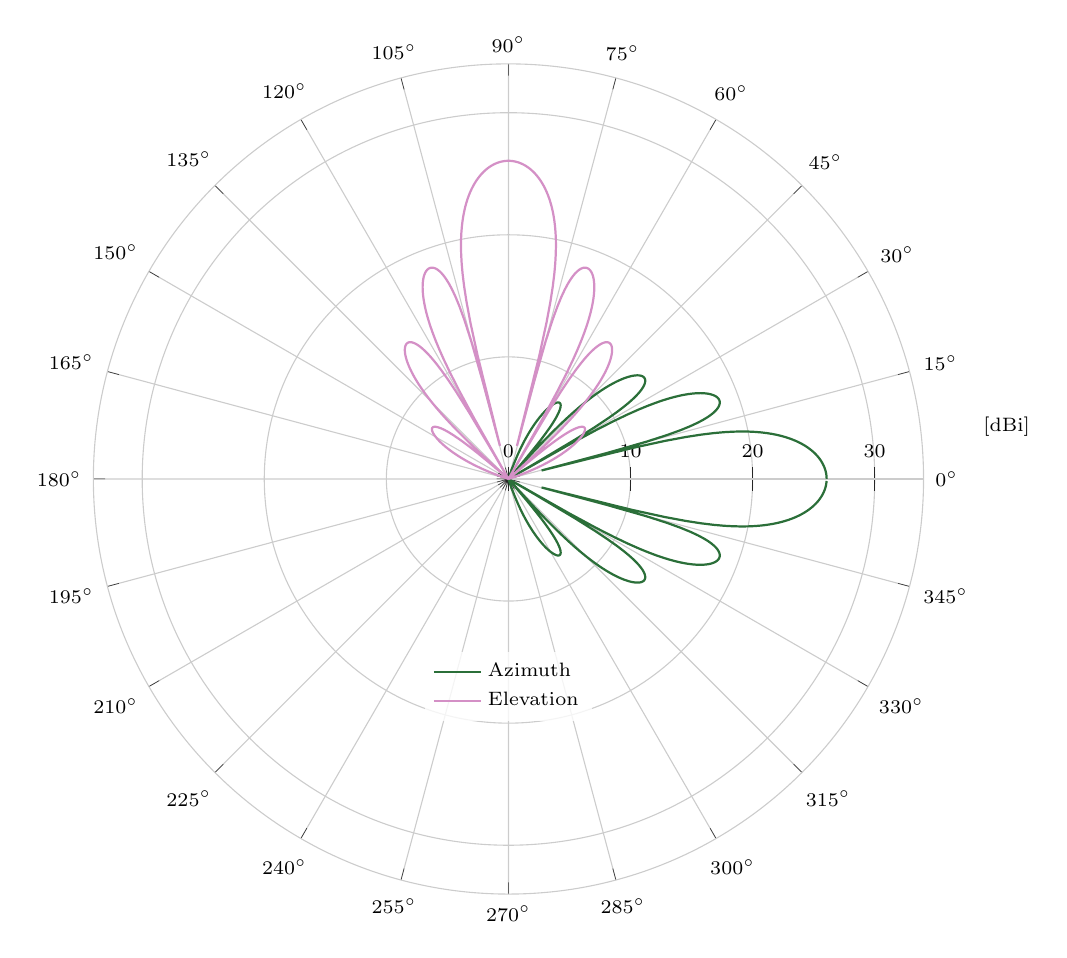
\begin{tikzpicture}

% \definecolor{color0}{rgb}{0.298039215686275,0.447058823529412,0.690196078431373}
% \definecolor{color1}{rgb}{0.866666666666667,0.517647058823529,0.32156862745098}
\definecolor{color0}{rgb}{0.17004232121058,0.436797596475173,0.223725555555555}
\definecolor{color1}{rgb}{0.82995767878942,0.563202403524827,0.776274444444444}


\begin{polaraxis}[
axis line style={white!80!black},
legend cell align={left},
legend style={fill opacity=0.8, draw opacity=1, text opacity=1, at={(0.5,0.25)}, anchor=center, draw=none},
tick align=outside,
tick pos=both,
x grid style={white!80!black},
xmajorgrids,
xmin=0, xmax=360,
xtick style={color=white!15!black},
xticklabel=$\pgfmathprintnumber{\tick}\si{\degree}$,
xticklabel shift=5pt,
y grid style={white!80!black},
ymajorgrids,
ymin=0, ymax=34,
ytick style={color=white!15!black},
ylabel={[dBi]},
ylabel style={at={(1.1,0.54)},anchor=south},
height=\linewidth,
scale=1
]
\addplot [thick, color0]
table {%
0 26.0617997398389
0.36 26.0569888215593
0.72 26.0425454974865
1.08 26.0184379342643
1.44 25.9846126541936
1.8 25.9409938905282
2.16 25.8874826612569
2.52 25.8239555364471
2.88 25.7502630651515
3.24 25.6662278171546
3.6 25.5716419818522
3.96 25.4662644505367
4.32 25.3498172882645
4.68 25.2219814759242
5.04 25.0823917701937
5.4 24.9306304861491
5.76 24.7662199506838
6.12 24.5886132993659
6.48 24.3971831873857
6.84 24.1912078458042
7.2 23.9698537210912
7.56 23.7321536643234
7.92 23.4769792486022
8.28 23.2030052300939
8.64 22.9086633349176
9 22.5920812958763
9.36 22.2510011189666
9.72 21.8826674781339
10.08 21.4836721096496
10.44 21.0497316033138
10.8 20.5753611558255
11.16 20.0533797354398
11.52 19.4741299243414
11.88 18.8241889412824
12.24 18.0841119810538
12.6 17.2241793649268
12.96 16.1955633196894
13.32 14.9093237752371
13.68 13.1751394724
14.04 10.4451652718033
14.4 2.80018113191606
14.76 8.28132883153452
15.12 11.7083681470774
15.48 13.492330173918
15.84 14.6700030699169
16.2 15.526568176237
16.56 16.1822157842005
16.92 16.6990038820005
17.28 17.1131452340716
17.64 17.4475831336526
18 17.7177361671918
18.36 17.9344305990977
18.72 18.1055254249803
19.08 18.2368718161868
19.44 18.3329086583768
19.8 18.3970473155065
20.16 18.4319282824336
20.52 18.4395966557751
20.88 18.4216241896851
21.24 18.3791949181031
21.6 18.3131649848267
21.96 18.2241034347186
22.32 18.1123182228181
22.68 17.977869999776
23.04 17.8205749793799
23.4 17.639997157804
23.76 17.4354291618325
24.12 17.2058598930157
24.48 16.949925714702
24.84 16.6658399247499
25.2 16.3512922264677
25.56 16.0033050877883
25.92 15.6180258623363
26.28 15.190419644397
26.64 14.7138026043195
27 14.1791073635279
27.36 13.5736741841315
27.72 12.8791482801764
28.08 12.067553220615
28.44 11.0932389701384
28.8 9.8740876898076
29.16 8.23828543701448
29.52 5.71414889449881
29.88 0
30.24 2.4957199808872
30.6 6.36086933152696
30.96 8.28109026677059
31.32 9.53644364317624
31.68 10.4494516724291
32.04 11.1516555322201
32.4 11.7098036233412
32.76 12.1624530228688
33.12 12.5338933476069
33.48 12.8404088078657
33.84 13.0934394831245
34.2 13.3013191987285
34.56 13.4702957468942
34.92 13.6051619006122
35.28 13.7096626173401
35.64 13.7867671825377
36 13.8388564732411
36.36 13.8678549852611
36.72 13.8753257982773
37.08 13.8625399793919
37.44 13.830527900433
37.8 13.7801174371676
38.16 13.7119624099975
38.52 13.6265635634901
38.88 13.5242836592637
39.24 13.4053577475365
39.6 13.2698993079056
39.96 13.1179026574262
40.32 12.9492417770581
40.68 12.7636654774042
41.04 12.5607885856507
41.4 12.3400785605145
41.76 12.1008365971546
42.12 11.8421718229446
42.48 11.5629665384276
42.84 11.2618295170062
43.2 10.9370329649459
43.56 10.5864265619047
43.92 10.207318532312
44.28 9.79630800331049
44.64 9.34904323007074
45 8.85986317299522
45.36 8.32124829506003
45.72 7.72294476421537
46.08 7.0504979257765
46.44 6.2826421321263
46.8 5.38627650132413
47.16 4.30572706324121
47.52 2.9361354403519
47.88 1.04045371742468
48.24 0
48.6 0
48.96 0
49.32 0.649947572625912
49.68 2.25402786972846
50.04 3.35184033923744
50.4 4.16898222966365
50.76 4.8066045866389
51.12 5.31888846798715
51.48 5.7382747638384
51.84 6.08574207932305
52.2 6.37564748154429
52.56 6.61825375286354
52.92 6.82115495756393
53.28 6.99013069818837
53.64 7.12968354892974
54 7.24339099075296
54.36 7.33414374816696
54.72 7.40431187685255
55.08 7.4558633910749
55.44 7.49045083093073
55.8 7.50947563693173
56.16 7.51413682797437
56.52 7.50546836275958
56.88 7.48436820156059
57.24 7.45162118635971
57.6 7.40791725212187
57.96 7.35386606665749
58.32 7.2900089066154
58.68 7.21682837158034
59.04 7.13475639038922
59.4 7.04418086601245
59.76 6.94545122584242
60.12 6.83888308491077
60.48 6.72476218483198
60.84 6.60334773721875
61.2 6.47487527415235
61.56 6.33955908801625
61.92 6.19759432716206
62.28 6.04915880140974
62.64 5.89441454149652
63 5.73350914869767
63.36 5.56657696449667
63.72 5.39374008505314
64.08 5.21510924103805
64.44 5.03078455998638
64.8 4.8408562254975
65.16 4.64540504527477
65.52 4.44450293804481
65.88 4.23821334775444
66.24 4.02659159205412
66.6 3.80968515088881
66.96 3.58753389999353
67.32 3.36017029319875
67.68 3.12761949666522
68.04 2.88989947746331
68.4 2.64702104827369
68.76 2.39898786939721
69.12 2.14579640870328
69.48 1.88743585961416
69.84 1.62388801669414
70.2 1.35512710788625
70.56 1.08111958189629
70.92 0.801823848656845
71.28 0.517189970197303
71.64 0.227159298587736
72 0
72.36 0
72.72 0
73.08 0
73.44 0
73.8 0
74.16 0
74.52 0
74.88 0
75.24 0
75.6 0
75.96 0
76.32 0
76.68 0
77.04 0
77.4 0
77.76 0
78.12 0
78.48 0
78.84 0
79.2 0
79.56 0
79.92 0
80.28 0
80.64 0
81 0
81.36 0
81.72 0
82.08 0
82.44 0
82.8 0
83.16 0
83.52 0
83.88 0
84.24 0
84.6 0
84.96 0
85.32 0
85.68 0
86.04 0
86.4 0
86.76 0
87.12 0
87.48 0
87.84 0
88.2 0
88.56 0
88.92 0
89.28 0
89.64 0
90 0
90.36 0
90.72 0
91.08 0
91.44 0
91.8 0
92.16 0
92.52 0
92.88 0
93.24 0
93.6 0
93.96 0
94.32 0
94.68 0
95.04 0
95.4 0
95.76 0
96.12 0
96.48 0
96.84 0
97.2 0
97.56 0
97.92 0
98.28 0
98.64 0
99 0
99.36 0
99.72 0
100.08 0
100.44 0
100.8 0
101.16 0
101.52 0
101.88 0
102.24 0
102.6 0
102.96 0
103.32 0
103.68 0
104.04 0
104.4 0
104.76 0
105.12 0
105.48 0
105.84 0
106.2 0
106.56 0
106.92 0
107.28 0
107.64 0
108 0
108.36 0
108.72 0
109.08 0
109.44 0
109.8 0
110.16 0
110.52 0
110.88 0
111.24 0
111.6 0
111.96 0
112.32 0
112.68 0
113.04 0
113.4 0
113.76 0
114.12 0
114.48 0
114.84 0
115.2 0
115.56 0
115.92 0
116.28 0
116.64 0
117 0
117.36 0
117.72 0
118.08 0
118.44 0
118.8 0
119.16 0
119.52 0
119.88 0
120.24 0
120.6 0
120.96 0
121.32 0
121.68 0
122.04 0
122.4 0
122.76 0
123.12 0
123.48 0
123.84 0
124.2 0
124.56 0
124.92 0
125.28 0
125.64 0
126 0
126.36 0
126.72 0
127.08 0
127.44 0
127.8 0
128.16 0
128.52 0
128.88 0
129.24 0
129.6 0
129.96 0
130.32 0
130.68 0
131.04 0
131.4 0
131.76 0
132.12 0
132.48 0
132.84 0
133.2 0
133.56 0
133.92 0
134.28 0
134.64 0
135 0
135.36 0
135.72 0
136.08 0
136.44 0
136.8 0
137.16 0
137.52 0
137.88 0
138.24 0
138.6 0
138.96 0
139.32 0
139.68 0
140.04 0
140.4 0
140.76 0
141.12 0
141.48 0
141.84 0
142.2 0
142.56 0
142.92 0
143.28 0
143.64 0
144 0
144.36 0
144.72 0
145.08 0
145.44 0
145.8 0
146.16 0
146.52 0
146.88 0
147.24 0
147.6 0
147.96 0
148.32 0
148.68 0
149.04 0
149.4 0
149.76 0
150.12 0
150.48 0
150.84 0
151.2 0
151.56 0
151.92 0
152.28 0
152.64 0
153 0
153.36 0
153.72 0
154.08 0
154.44 0
154.8 0
155.16 0
155.52 0
155.88 0
156.24 0
156.6 0
156.96 0
157.32 0
157.68 0
158.04 0
158.4 0
158.76 0
159.12 0
159.48 0
159.84 0
160.2 0
160.56 0
160.92 0
161.28 0
161.64 0
162 0
162.36 0
162.72 0
163.08 0
163.44 0
163.8 0
164.16 0
164.52 0
164.88 0
165.24 0
165.6 0
165.96 0
166.32 0
166.68 0
167.04 0
167.4 0
167.76 0
168.12 0
168.48 0
168.84 0
169.2 0
169.56 0
169.92 0
170.28 0
170.64 0
171 0
171.36 0
171.72 0
172.08 0
172.44 0
172.8 0
173.16 0
173.52 0
173.88 0
174.24 0
174.6 0
174.96 0
175.32 0
175.68 0
176.04 0
176.4 0
176.76 0
177.12 0
177.48 0
177.84 0
178.2 0
178.56 0
178.92 0
179.28 0
179.64 0
180 0
180.36 0
180.72 0
181.08 0
181.44 0
181.8 0
182.16 0
182.52 0
182.88 0
183.24 0
183.6 0
183.96 0
184.32 0
184.68 0
185.04 0
185.4 0
185.76 0
186.12 0
186.48 0
186.84 0
187.2 0
187.56 0
187.92 0
188.28 0
188.64 0
189 0
189.36 0
189.72 0
190.08 0
190.44 0
190.8 0
191.16 0
191.52 0
191.88 0
192.24 0
192.6 0
192.96 0
193.32 0
193.68 0
194.04 0
194.4 0
194.76 0
195.12 0
195.48 0
195.84 0
196.2 0
196.56 0
196.92 0
197.28 0
197.64 0
198 0
198.36 0
198.72 0
199.08 0
199.44 0
199.8 0
200.16 0
200.52 0
200.88 0
201.24 0
201.6 0
201.96 0
202.32 0
202.68 0
203.04 0
203.4 0
203.76 0
204.12 0
204.48 0
204.84 0
205.2 0
205.56 0
205.92 0
206.28 0
206.64 0
207 0
207.36 0
207.72 0
208.08 0
208.44 0
208.8 0
209.16 0
209.52 0
209.88 0
210.24 0
210.6 0
210.96 0
211.32 0
211.68 0
212.04 0
212.4 0
212.76 0
213.12 0
213.48 0
213.84 0
214.2 0
214.56 0
214.92 0
215.28 0
215.64 0
216 0
216.36 0
216.72 0
217.08 0
217.44 0
217.8 0
218.16 0
218.52 0
218.88 0
219.24 0
219.6 0
219.96 0
220.32 0
220.68 0
221.04 0
221.4 0
221.76 0
222.12 0
222.48 0
222.84 0
223.2 0
223.56 0
223.92 0
224.28 0
224.64 0
225 0
225.36 0
225.72 0
226.08 0
226.44 0
226.8 0
227.16 0
227.52 0
227.88 0
228.24 0
228.6 0
228.96 0
229.32 0
229.68 0
230.04 0
230.4 0
230.76 0
231.12 0
231.48 0
231.84 0
232.2 0
232.56 0
232.92 0
233.28 0
233.64 0
234 0
234.36 0
234.72 0
235.08 0
235.44 0
235.8 0
236.16 0
236.52 0
236.88 0
237.24 0
237.6 0
237.96 0
238.32 0
238.68 0
239.04 0
239.4 0
239.76 0
240.12 0
240.48 0
240.84 0
241.2 0
241.56 0
241.92 0
242.28 0
242.64 0
243 0
243.36 0
243.72 0
244.08 0
244.44 0
244.8 0
245.16 0
245.52 0
245.88 0
246.24 0
246.6 0
246.96 0
247.32 0
247.68 0
248.04 0
248.4 0
248.76 0
249.12 0
249.48 0
249.84 0
250.2 0
250.56 0
250.92 0
251.28 0
251.64 0
252 0
252.36 0
252.72 0
253.08 0
253.44 0
253.8 0
254.16 0
254.52 0
254.88 0
255.24 0
255.6 0
255.96 0
256.32 0
256.68 0
257.04 0
257.4 0
257.76 0
258.12 0
258.48 0
258.84 0
259.2 0
259.56 0
259.92 0
260.28 0
260.64 0
261 0
261.36 0
261.72 0
262.08 0
262.44 0
262.8 0
263.16 0
263.52 0
263.88 0
264.24 0
264.6 0
264.96 0
265.32 0
265.68 0
266.04 0
266.4 0
266.76 0
267.12 0
267.48 0
267.84 0
268.2 0
268.56 0
268.92 0
269.28 0
269.64 0
270 0
270.36 0
270.72 0
271.08 0
271.44 0
271.8 0
272.16 0
272.52 0
272.88 0
273.24 0
273.6 0
273.96 0
274.32 0
274.68 0
275.04 0
275.4 0
275.76 0
276.12 0
276.48 0
276.84 0
277.2 0
277.56 0
277.92 0
278.28 0
278.64 0
279 0
279.36 0
279.72 0
280.08 0
280.44 0
280.8 0
281.16 0
281.52 0
281.88 0
282.24 0
282.6 0
282.96 0
283.32 0
283.68 0
284.04 0
284.4 0
284.76 0
285.12 0
285.48 0
285.84 0
286.2 0
286.56 0
286.92 0
287.28 0
287.64 0
288 0
288.36 0.227159298587736
288.72 0.517189970197236
289.08 0.801823848656907
289.44 1.08111958189629
289.8 1.35512710788634
290.16 1.62388801669421
290.52 1.88743585961419
290.88 2.14579640870328
291.24 2.39898786939721
291.6 2.64702104827369
291.96 2.88989947746327
292.32 3.12761949666525
292.68 3.36017029319875
293.04 3.58753389999359
293.4 3.80968515088889
293.76 4.02659159205415
294.12 4.23821334775444
294.48 4.44450293804481
294.84 4.64540504527477
295.2 4.84085622549747
295.56 5.0307845599864
295.92 5.21510924103805
296.28 5.39374008505314
296.64 5.5665769644967
297 5.73350914869768
297.36 5.89441454149655
297.72 6.04915880140974
298.08 6.19759432716206
298.44 6.33955908801622
298.8 6.47487527415237
299.16 6.60334773721875
299.52 6.72476218483198
299.88 6.8388830849108
300.24 6.94545122584243
300.6 7.04418086601246
300.96 7.13475639038922
301.32 7.21682837158034
301.68 7.2900089066154
302.04 7.35386606665751
302.4 7.40791725212187
302.76 7.45162118635971
303.12 7.4843682015606
303.48 7.50546836275957
303.84 7.51413682797436
304.2 7.50947563693173
304.56 7.49045083093073
304.92 7.45586339107491
305.28 7.40431187685256
305.64 7.33414374816696
306 7.24339099075296
306.36 7.1296835489297
306.72 6.99013069818834
307.08 6.82115495756389
307.44 6.61825375286354
307.8 6.37564748154429
308.16 6.08574207932312
308.52 5.73827476383847
308.88 5.31888846798715
309.24 4.8066045866389
309.6 4.16898222966342
309.96 3.35184033923734
310.32 2.25402786972825
310.68 0.649947572625912
311.04 0
311.4 0
311.76 0
312.12 1.04045371742498
312.48 2.9361354403519
312.84 4.30572706324153
313.2 5.38627650132422
313.56 6.28264213212645
313.92 7.05049792577656
314.28 7.72294476421537
314.64 8.32124829505998
315 8.85986317299514
315.36 9.34904323007077
315.72 9.79630800331049
316.08 10.2073185323121
316.44 10.5864265619047
316.8 10.9370329649459
317.16 11.2618295170062
317.52 11.5629665384276
317.88 11.8421718229446
318.24 12.1008365971546
318.6 12.3400785605146
318.96 12.5607885856507
319.32 12.7636654774042
319.68 12.9492417770582
320.04 13.1179026574262
320.4 13.2698993079056
320.76 13.4053577475365
321.12 13.5242836592637
321.48 13.6265635634901
321.84 13.7119624099975
322.2 13.7801174371676
322.56 13.830527900433
322.92 13.8625399793919
323.28 13.8753257982773
323.64 13.8678549852611
324 13.8388564732411
324.36 13.7867671825377
324.72 13.7096626173401
325.08 13.6051619006121
325.44 13.4702957468942
325.8 13.3013191987284
326.16 13.0934394831244
326.52 12.8404088078657
326.88 12.5338933476069
327.24 12.1624530228688
327.6 11.7098036233412
327.96 11.1516555322202
328.32 10.449451672429
328.68 9.53644364317614
329.04 8.28109026677025
329.4 6.36086933152643
329.76 2.49571998088656
330.12 0
330.48 5.71414889449881
330.84 8.23828543701437
331.2 9.87408768980743
331.56 11.0932389701385
331.92 12.0675532206151
332.28 12.8791482801767
332.64 13.5736741841316
333 14.179107363528
333.36 14.7138026043195
333.72 15.190419644397
334.08 15.6180258623363
334.44 16.0033050877883
334.8 16.3512922264678
335.16 16.6658399247499
335.52 16.949925714702
335.88 17.2058598930157
336.24 17.4354291618325
336.6 17.639997157804
336.96 17.8205749793799
337.32 17.977869999776
337.68 18.1123182228181
338.04 18.2241034347186
338.4 18.3131649848267
338.76 18.3791949181031
339.12 18.4216241896851
339.48 18.4395966557751
339.84 18.4319282824336
340.2 18.3970473155065
340.56 18.3329086583768
340.92 18.2368718161868
341.28 18.1055254249803
341.64 17.9344305990977
342 17.7177361671918
342.36 17.4475831336525
342.72 17.1131452340716
343.08 16.6990038820005
343.44 16.1822157842005
343.8 15.526568176237
344.16 14.6700030699169
344.52 13.4923301739182
344.88 11.7083681470772
345.24 8.28132883153452
345.6 2.80018113192029
345.96 10.4451652718039
346.32 13.1751394724002
346.68 14.9093237752372
347.04 16.1955633196894
347.4 17.2241793649268
347.76 18.0841119810537
348.12 18.8241889412824
348.48 19.4741299243414
348.84 20.0533797354399
349.2 20.5753611558256
349.56 21.0497316033139
349.92 21.4836721096497
350.28 21.8826674781339
350.64 22.2510011189665
351 22.5920812958762
351.36 22.9086633349176
351.72 23.2030052300939
352.08 23.4769792486023
352.44 23.7321536643234
352.8 23.9698537210913
353.16 24.1912078458042
353.52 24.3971831873857
353.88 24.5886132993659
354.24 24.7662199506838
354.6 24.9306304861491
354.96 25.0823917701937
355.32 25.2219814759243
355.68 25.3498172882645
356.04 25.4662644505367
356.4 25.5716419818523
356.76 25.6662278171546
357.12 25.7502630651515
357.48 25.8239555364471
357.84 25.8874826612569
358.2 25.9409938905282
358.56 25.9846126541936
358.92 26.0184379342643
359.28 26.0425454974865
359.64 26.0569888215593
};
\addlegendentry{Azimuth}
\addplot [thick, color1]
table {%
0 0
0.36 0
0.72 0
1.08 0
1.44 0
1.8 0
2.16 0
2.52 0
2.88 0
3.24 0
3.6 0
3.96 0
4.32 0
4.68 0
5.04 0
5.4 0
5.76 0
6.12 0
6.48 0
6.84 0
7.2 0
7.56 0
7.92 0
8.28 0
8.64 0
9 0
9.36 0
9.72 0
10.08 0
10.44 0
10.8 0
11.16 0
11.52 0
11.88 0
12.24 0
12.6 0
12.96 0
13.32 0
13.68 0
14.04 0
14.4 0
14.76 0
15.12 0
15.48 0
15.84 0
16.2 0
16.56 0
16.92 0
17.28 0
17.64 0
18 0
18.36 0.227159298587752
18.72 0.517189970197288
19.08 0.801823848656875
19.44 1.08111958189628
19.8 1.35512710788626
20.16 1.62388801669416
20.52 1.88743585961419
20.88 2.14579640870328
21.24 2.39898786939721
21.6 2.64702104827372
21.96 2.88989947746331
22.32 3.12761949666523
22.68 3.36017029319874
23.04 3.58753389999354
23.4 3.80968515088885
23.76 4.02659159205412
24.12 4.23821334775443
24.48 4.44450293804481
24.84 4.64540504527478
25.2 4.8408562254975
25.56 5.03078455998638
25.92 5.21510924103805
26.28 5.39374008505314
26.64 5.56657696449668
27 5.73350914869767
27.36 5.89441454149654
27.72 6.04915880140974
28.08 6.19759432716207
28.44 6.33955908801624
28.8 6.47487527415235
29.16 6.60334773721874
29.52 6.72476218483198
29.88 6.83888308491077
30.24 6.94545122584242
30.6 7.04418086601245
30.96 7.13475639038922
31.32 7.21682837158035
31.68 7.2900089066154
32.04 7.3538660666575
32.4 7.40791725212186
32.76 7.45162118635971
33.12 7.48436820156059
33.48 7.50546836275958
33.84 7.51413682797437
34.2 7.50947563693173
34.56 7.49045083093074
34.92 7.4558633910749
35.28 7.40431187685256
35.64 7.33414374816696
36 7.24339099075296
36.36 7.12968354892972
36.72 6.99013069818836
37.08 6.82115495756392
37.44 6.61825375286355
37.8 6.37564748154428
38.16 6.08574207932308
38.52 5.7382747638384
38.88 5.3188884679872
39.24 4.8066045866389
39.6 4.16898222966354
39.96 3.35184033923748
40.32 2.25402786972843
40.68 0.649947572625852
41.04 0
41.4 0
41.76 0
42.12 1.04045371742468
42.48 2.9361354403519
42.84 4.30572706324128
43.2 5.38627650132408
43.56 6.28264213212634
43.92 7.05049792577652
44.28 7.72294476421537
44.64 8.32124829506003
45 8.85986317299521
45.36 9.34904323007074
45.72 9.79630800331046
46.08 10.207318532312
46.44 10.5864265619047
46.8 10.9370329649459
47.16 11.2618295170062
47.52 11.5629665384276
47.88 11.8421718229446
48.24 12.1008365971546
48.6 12.3400785605145
48.96 12.5607885856507
49.32 12.7636654774042
49.68 12.9492417770581
50.04 13.1179026574262
50.4 13.2698993079056
50.76 13.4053577475365
51.12 13.5242836592637
51.48 13.6265635634902
51.84 13.7119624099975
52.2 13.7801174371676
52.56 13.830527900433
52.92 13.8625399793919
53.28 13.8753257982773
53.64 13.8678549852611
54 13.8388564732411
54.36 13.7867671825377
54.72 13.7096626173401
55.08 13.6051619006121
55.44 13.4702957468942
55.8 13.3013191987285
56.16 13.0934394831245
56.52 12.8404088078657
56.88 12.5338933476069
57.24 12.1624530228688
57.6 11.7098036233412
57.96 11.1516555322201
58.32 10.4494516724291
58.68 9.53644364317619
59.04 8.28109026677056
59.4 6.36086933152679
59.76 2.49571998088734
60.12 0
60.48 5.71414889449881
60.84 8.23828543701448
61.2 9.87408768980757
61.56 11.0932389701384
61.92 12.067553220615
62.28 12.8791482801765
62.64 13.5736741841315
63 14.1791073635279
63.36 14.7138026043195
63.72 15.190419644397
64.08 15.6180258623363
64.44 16.0033050877883
64.8 16.3512922264677
65.16 16.6658399247499
65.52 16.949925714702
65.88 17.2058598930157
66.24 17.4354291618325
66.6 17.639997157804
66.96 17.8205749793799
67.32 17.977869999776
67.68 18.1123182228181
68.04 18.2241034347186
68.4 18.3131649848267
68.76 18.3791949181031
69.12 18.4216241896851
69.48 18.4395966557751
69.84 18.4319282824336
70.2 18.3970473155065
70.56 18.3329086583768
70.92 18.2368718161868
71.28 18.1055254249803
71.64 17.9344305990977
72 17.7177361671918
72.36 17.4475831336526
72.72 17.1131452340716
73.08 16.6990038820005
73.44 16.1822157842006
73.8 15.526568176237
74.16 14.6700030699168
74.52 13.492330173918
74.88 11.7083681470774
75.24 8.28132883153452
75.6 2.80018113191606
75.96 10.4451652718033
76.32 13.1751394724
76.68 14.9093237752372
77.04 16.1955633196895
77.4 17.2241793649269
77.76 18.0841119810538
78.12 18.8241889412824
78.48 19.4741299243414
78.84 20.0533797354398
79.2 20.5753611558255
79.56 21.0497316033139
79.92 21.4836721096497
80.28 21.8826674781339
80.64 22.2510011189666
81 22.5920812958763
81.36 22.9086633349176
81.72 23.2030052300939
82.08 23.4769792486022
82.44 23.7321536643234
82.8 23.9698537210913
83.16 24.1912078458042
83.52 24.3971831873857
83.88 24.5886132993659
84.24 24.7662199506838
84.6 24.9306304861491
84.96 25.0823917701937
85.32 25.2219814759242
85.68 25.3498172882645
86.04 25.4662644505367
86.4 25.5716419818523
86.76 25.6662278171546
87.12 25.7502630651515
87.48 25.8239555364471
87.84 25.8874826612569
88.2 25.9409938905282
88.56 25.9846126541936
88.92 26.0184379342643
89.28 26.0425454974865
89.64 26.0569888215593
90 26.0617997398389
90.36 26.0569888215593
90.72 26.0425454974865
91.08 26.0184379342643
91.44 25.9846126541936
91.8 25.9409938905282
92.16 25.8874826612569
92.52 25.8239555364471
92.88 25.7502630651515
93.24 25.6662278171546
93.6 25.5716419818522
93.96 25.4662644505367
94.32 25.3498172882645
94.68 25.2219814759242
95.04 25.0823917701937
95.4 24.9306304861491
95.76 24.7662199506838
96.12 24.5886132993659
96.48 24.3971831873857
96.84 24.1912078458042
97.2 23.9698537210912
97.56 23.7321536643234
97.92 23.4769792486022
98.28 23.2030052300939
98.64 22.9086633349175
99 22.5920812958763
99.36 22.2510011189666
99.72 21.8826674781339
100.08 21.4836721096496
100.44 21.0497316033138
100.8 20.5753611558255
101.16 20.0533797354398
101.52 19.4741299243414
101.88 18.8241889412824
102.24 18.0841119810538
102.6 17.2241793649268
102.96 16.1955633196894
103.32 14.9093237752371
103.68 13.1751394724
104.04 10.4451652718032
104.4 2.80018113191525
104.76 8.28132883153473
105.12 11.7083681470774
105.48 13.492330173918
105.84 14.6700030699169
106.2 15.526568176237
106.56 16.1822157842006
106.92 16.6990038820005
107.28 17.1131452340716
107.64 17.4475831336526
108 17.7177361671918
108.36 17.9344305990977
108.72 18.1055254249803
109.08 18.2368718161868
109.44 18.3329086583768
109.8 18.3970473155065
110.16 18.4319282824336
110.52 18.4395966557751
110.88 18.4216241896851
111.24 18.3791949181031
111.6 18.3131649848267
111.96 18.2241034347186
112.32 18.1123182228181
112.68 17.977869999776
113.04 17.8205749793799
113.4 17.639997157804
113.76 17.4354291618324
114.12 17.2058598930157
114.48 16.949925714702
114.84 16.6658399247499
115.2 16.3512922264677
115.56 16.0033050877883
115.92 15.6180258623363
116.28 15.1904196443969
116.64 14.7138026043195
117 14.1791073635279
117.36 13.5736741841315
117.72 12.8791482801764
118.08 12.067553220615
118.44 11.0932389701383
118.8 9.87408768980749
119.16 8.23828543701432
119.52 5.71414889449881
119.88 0
120.24 2.49571998088734
120.6 6.36086933152694
120.96 8.28109026677064
121.32 9.53644364317623
121.68 10.4494516724291
122.04 11.1516555322202
122.4 11.7098036233412
122.76 12.1624530228688
123.12 12.5338933476069
123.48 12.8404088078657
123.84 13.0934394831245
124.2 13.3013191987285
124.56 13.4702957468942
124.92 13.6051619006122
125.28 13.7096626173401
125.64 13.7867671825377
126 13.8388564732411
126.36 13.8678549852611
126.72 13.8753257982773
127.08 13.8625399793919
127.44 13.830527900433
127.8 13.7801174371676
128.16 13.7119624099975
128.52 13.6265635634902
128.88 13.5242836592637
129.24 13.4053577475365
129.6 13.2698993079056
129.96 13.1179026574262
130.32 12.9492417770581
130.68 12.7636654774042
131.04 12.5607885856506
131.4 12.3400785605145
131.76 12.1008365971546
132.12 11.8421718229446
132.48 11.5629665384276
132.84 11.2618295170062
133.2 10.9370329649459
133.56 10.5864265619047
133.92 10.207318532312
134.28 9.79630800331045
134.64 9.34904323007074
135 8.85986317299522
135.36 8.32124829506002
135.72 7.72294476421537
136.08 7.0504979257765
136.44 6.28264213212634
136.8 5.38627650132405
137.16 4.30572706324121
137.52 2.9361354403519
137.88 1.04045371742474
138.24 0
138.6 0
138.96 0
139.32 0.649947572625846
139.68 2.25402786972847
140.04 3.35184033923754
140.4 4.16898222966362
140.76 4.80660458663887
141.12 5.3188884679872
141.48 5.7382747638384
141.84 6.08574207932308
142.2 6.37564748154429
142.56 6.61825375286355
142.92 6.82115495756393
143.28 6.99013069818836
143.64 7.12968354892973
144 7.24339099075295
144.36 7.33414374816696
144.72 7.40431187685256
145.08 7.45586339107491
145.44 7.49045083093074
145.8 7.50947563693173
146.16 7.51413682797437
146.52 7.50546836275958
146.88 7.48436820156059
147.24 7.45162118635971
147.6 7.40791725212187
147.96 7.35386606665749
148.32 7.2900089066154
148.68 7.21682837158034
149.04 7.13475639038921
149.4 7.04418086601245
149.76 6.94545122584242
150.12 6.83888308491077
150.48 6.72476218483198
150.84 6.60334773721874
151.2 6.47487527415234
151.56 6.33955908801624
151.92 6.19759432716206
152.28 6.04915880140973
152.64 5.89441454149654
153 5.73350914869767
153.36 5.56657696449667
153.72 5.39374008505314
154.08 5.21510924103804
154.44 5.03078455998638
154.8 4.84085622549749
155.16 4.64540504527477
155.52 4.44450293804481
155.88 4.23821334775443
156.24 4.02659159205412
156.6 3.80968515088885
156.96 3.58753389999353
157.32 3.36017029319873
157.68 3.12761949666522
158.04 2.8898994774633
158.4 2.6470210482737
158.76 2.39898786939721
159.12 2.14579640870328
159.48 1.88743585961419
159.84 1.62388801669416
160.2 1.35512710788625
160.56 1.08111958189628
160.92 0.801823848656845
161.28 0.517189970197277
161.64 0.227159298587742
162 0
162.36 0
162.72 0
163.08 0
163.44 0
163.8 0
164.16 0
164.52 0
164.88 0
165.24 0
165.6 0
165.96 0
166.32 0
166.68 0
167.04 0
167.4 0
167.76 0
168.12 0
168.48 0
168.84 0
169.2 0
169.56 0
169.92 0
170.28 0
170.64 0
171 0
171.36 0
171.72 0
172.08 0
172.44 0
172.8 0
173.16 0
173.52 0
173.88 0
174.24 0
174.6 0
174.96 0
175.32 0
175.68 0
176.04 0
176.4 0
176.76 0
177.12 0
177.48 0
177.84 0
178.2 0
178.56 0
178.92 0
179.28 0
179.64 0
};
\addlegendentry{Elevation}
\end{polaraxis}

\end{tikzpicture}

\caption{8 by 8 antenna array}
\end{subfigure}~
\begin{subfigure}[t]{0.5\linewidth}
% This file was created by tikzplotlib v0.9.3.
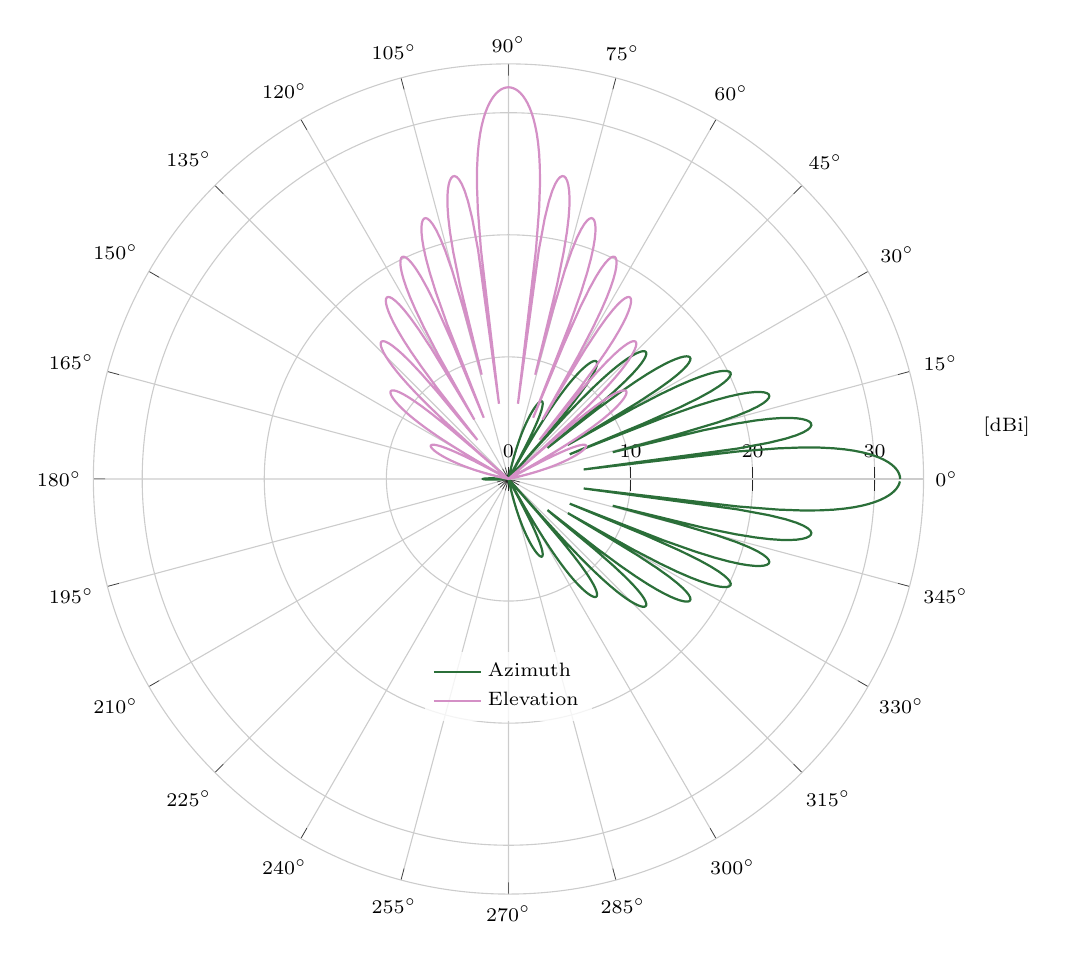
\begin{tikzpicture}

% \definecolor{color0}{rgb}{0.298039215686275,0.447058823529412,0.690196078431373}
% \definecolor{color1}{rgb}{0.866666666666667,0.517647058823529,0.32156862745098}
\definecolor{color0}{rgb}{0.17004232121058,0.436797596475173,0.223725555555555}
\definecolor{color1}{rgb}{0.82995767878942,0.563202403524827,0.776274444444444}

\begin{polaraxis}[
axis line style={white!80!black},
legend cell align={left},
legend style={fill opacity=0.8, draw opacity=1, text opacity=1, at={(0.5,0.25)}, anchor=center, draw=none},
tick align=outside,
tick pos=both,
x grid style={white!80!black},
xmajorgrids,
xmin=0, xmax=360,
xtick style={color=white!15!black},
xticklabel=$\pgfmathprintnumber{\tick}\si{\degree}$,
xticklabel shift=5pt,
y grid style={white!80!black},
ymajorgrids,
ymin=0, ymax=34,
ytick style={color=white!15!black},
ylabel={[dBi]},
ylabel style={at={(1.1,0.54)},anchor=south},
height=\linewidth,
scale=1
]
\addplot [thick, color0]
table {%
0 32.0823996531185
0.36 32.0640374703733
0.72 32.0087723101197
1.08 31.9160597023953
1.44 31.7849624855818
1.8 31.6141027989668
2.16 31.4015872983053
2.52 31.144896180777
2.88 30.8407206205592
3.24 30.4847232423143
3.6 30.0711787728817
3.96 29.5924197557253
4.32 29.0379492881516
4.68 28.3929516841029
5.04 27.635636423792
5.4 26.7321143150029
5.76 25.6254139005333
6.12 24.2081364259238
6.48 22.2364928050294
6.84 18.9105330401289
7.2 6.21002696606593
7.56 18.9118490500104
7.92 21.5397670268885
8.28 22.9643150840172
8.64 23.8667962190973
9 24.4653027813559
9.36 24.8567291551208
9.72 25.0915411255972
10.08 25.1981904489882
10.44 25.1929474174249
10.8 25.0843241577734
11.16 24.8750638253396
11.52 24.5627625474867
11.88 24.1394200228019
12.24 23.589709598768
12.6 22.8870683017119
12.96 21.9850932407618
13.32 20.7966942875485
13.68 19.1329334568944
14.04 16.4469566571451
14.4 8.8201924576529
14.76 14.2941196039894
15.12 17.6885382809797
15.48 19.4142243618701
15.84 20.5074020106471
16.2 21.2523512369304
16.56 21.7679766274251
16.92 22.1145952796091
17.28 22.3261206430721
17.64 22.4224886939775
18 22.4151841155851
18.36 22.3098471975154
18.72 22.1074007990028
19.08 21.8042198429517
19.44 21.3914160054886
19.8 20.8529189834715
20.16 20.1613755975515
20.52 19.2692336911643
20.88 18.0871123083963
21.24 16.4198231154074
21.6 13.6934685330337
21.96 5.41032706321655
22.32 11.9158629494291
22.68 15.2242519563341
23.04 16.944045718869
23.4 18.0498056093835
23.76 18.8157889928531
24.12 19.3580902031556
24.48 19.7362072565348
24.84 19.9840476907507
25.2 20.1220189531564
25.56 20.1624808653364
25.92 20.1124046641693
26.28 19.9746593685421
26.64 19.7484884798602
27 19.4293625429372
27.36 19.0081509495815
27.72 18.4692742524838
28.08 17.786953043244
28.44 16.9172792994284
28.8 15.7795101434303
29.16 14.20290279342
29.52 11.7165867139373
29.88 5.61236870618995
30.24 8.51181681938962
30.6 12.3533771887464
30.96 14.2297985909568
31.32 15.4209599969783
31.68 16.2490066470197
32.04 16.8448916401154
32.4 17.2745390690126
32.76 17.575409025543
33.12 17.7703702418577
33.48 17.8738908849222
33.84 17.8951004677183
34.2 17.839387684429
34.56 17.7092198427079
34.92 17.5044792958354
35.28 17.2224257816772
35.64 16.8572724069844
36 16.3992347696566
36.36 15.832698215157
36.72 15.1326784787291
37.08 14.2575316350404
37.44 13.1321300594389
37.8 11.6014089547627
38.16 9.25604916222058
38.52 4.08698490468764
38.88 4.83587426263997
39.24 9.20255567911807
39.6 11.2075512454762
39.96 12.4650842941976
40.32 13.341453374228
40.68 13.9805566897952
41.04 14.4537607006544
41.4 14.8014899026178
41.76 15.048646745713
42.12 15.2114168788537
42.48 15.3006430463387
42.84 15.3236360368665
43.2 15.2851949305638
43.56 15.1881877357914
43.92 15.0338609896038
44.28 14.8219577844422
44.64 14.5506723401596
45 14.2164300954934
45.36 13.8134384300787
45.72 13.332884354448
46.08 12.7615229304237
46.44 12.0791087715587
46.8 11.2534037795047
47.16 10.2294640636453
47.52 8.90304794813864
47.88 7.03762597861826
48.24 3.8660098878071
48.6 0
48.96 3.84429910598927
49.32 6.64652674441483
49.68 8.22132281760655
50.04 9.27848789134729
50.4 10.0436630886687
50.76 10.6179862511438
51.12 11.0555670293136
51.48 11.3887143441017
51.84 11.6382105688674
52.2 11.818147061154
52.56 11.9384444348167
52.92 12.0062690282685
53.28 12.0268754624948
53.64 12.0041291163315
54 11.9408389391463
54.36 11.8389712515848
54.72 11.699784139039
55.08 11.5239047562737
55.44 11.3113613862436
55.8 11.061574900174
56.16 10.7733082837016
56.52 10.4445665645299
56.88 10.0724310976901
57.24 9.65279915608162
57.6 9.1799773863474
57.96 8.64603615247587
58.32 8.03974927933577
58.68 7.34476729253926
59.04 6.53626056227443
59.4 5.57419600814289
59.76 4.38817493991625
60.12 2.83674053325935
60.48 0.561895056213575
60.84 0
61.2 0
61.56 0
61.92 1.83222053105593
62.28 3.14919868285735
62.64 4.07215030173231
63 4.75985334818133
63.36 5.28975965799228
63.72 5.70555524272014
64.08 6.03434598164386
64.44 6.29413140216266
64.8 6.49748878365306
65.16 6.65356272635827
65.52 6.76921725738216
65.88 6.84974087838547
66.24 6.89929784292702
66.6 6.92122796485645
66.96 6.91825215244787
67.32 6.89261714549471
67.68 6.84619982955917
68.04 6.78058395069394
68.4 6.69711754106308
68.76 6.59695658142523
69.12 6.48109865950294
69.48 6.35040923367947
69.84 6.20564234662446
70.2 6.04745711422619
70.56 5.87643095620635
70.92 5.6930702823788
71.28 5.4978191682753
71.64 5.29106642329594
72 5.07315135866319
72.36 4.84436849112728
72.72 4.60497136461964
73.08 4.35517563101514
73.44 4.0951614994085
73.8 3.82507563836744
74.16 3.54503259569562
74.52 3.25511578399903
74.88 2.95537806678562
75.24 2.64584196817687
75.6 2.32649951893674
75.96 1.99731174192894
76.32 1.65820777082741
76.68 1.3090835865275
77.04 0.949800345794303
77.4 0.580182265811063
77.76 0.200014015930661
78.12 0
78.48 0
78.84 0
79.2 0
79.56 0
79.92 0
80.28 0
80.64 0
81 0
81.36 0
81.72 0
82.08 0
82.44 0
82.8 0
83.16 0
83.52 0
83.88 0
84.24 0
84.6 0
84.96 0
85.32 0
85.68 0
86.04 0
86.4 0
86.76 0
87.12 0
87.48 0
87.84 0
88.2 0
88.56 0
88.92 0
89.28 0
89.64 0
90 0
90.36 0
90.72 0
91.08 0
91.44 0
91.8 0
92.16 0
92.52 0
92.88 0
93.24 0
93.6 0
93.96 0
94.32 0
94.68 0
95.04 0
95.4 0
95.76 0
96.12 0
96.48 0
96.84 0
97.2 0
97.56 0
97.92 0
98.28 0
98.64 0
99 0
99.36 0
99.72 0
100.08 0
100.44 0
100.8 0
101.16 0
101.52 0
101.88 0
102.24 0
102.6 0
102.96 0
103.32 0
103.68 0
104.04 0
104.4 0
104.76 0
105.12 0
105.48 0
105.84 0
106.2 0
106.56 0
106.92 0
107.28 0
107.64 0
108 0
108.36 0
108.72 0
109.08 0
109.44 0
109.8 0
110.16 0
110.52 0
110.88 0
111.24 0
111.6 0
111.96 0
112.32 0
112.68 0
113.04 0
113.4 0
113.76 0
114.12 0
114.48 0
114.84 0
115.2 0
115.56 0
115.92 0
116.28 0
116.64 0
117 0
117.36 0
117.72 0
118.08 0
118.44 0
118.8 0
119.16 0
119.52 0
119.88 0
120.24 0
120.6 0
120.96 0
121.32 0
121.68 0
122.04 0
122.4 0
122.76 0
123.12 0
123.48 0
123.84 0
124.2 0
124.56 0
124.92 0
125.28 0
125.64 0
126 0
126.36 0
126.72 0
127.08 0
127.44 0
127.8 0
128.16 0
128.52 0
128.88 0
129.24 0
129.6 0
129.96 0
130.32 0
130.68 0
131.04 0
131.4 0
131.76 0
132.12 0
132.48 0
132.84 0
133.2 0
133.56 0
133.92 0
134.28 0
134.64 0
135 0
135.36 0
135.72 0
136.08 0
136.44 0
136.8 0
137.16 0
137.52 0
137.88 0
138.24 0
138.6 0
138.96 0
139.32 0
139.68 0
140.04 0
140.4 0
140.76 0
141.12 0
141.48 0
141.84 0
142.2 0
142.56 0
142.92 0
143.28 0
143.64 0
144 0
144.36 0
144.72 0
145.08 0
145.44 0
145.8 0
146.16 0
146.52 0
146.88 0
147.24 0
147.6 0
147.96 0
148.32 0
148.68 0
149.04 0
149.4 0
149.76 0
150.12 0
150.48 0
150.84 0
151.2 0
151.56 0
151.92 0
152.28 0
152.64 0
153 0
153.36 0
153.72 0
154.08 0
154.44 0
154.8 0
155.16 0
155.52 0
155.88 0
156.24 0
156.6 0
156.96 0
157.32 0
157.68 0
158.04 0
158.4 0
158.76 0
159.12 0
159.48 0
159.84 0
160.2 0
160.56 0
160.92 0
161.28 0
161.64 0
162 0
162.36 0
162.72 0
163.08 0
163.44 0
163.8 0
164.16 0
164.52 0
164.88 0
165.24 0
165.6 0
165.96 0
166.32 0
166.68 0
167.04 0
167.4 0
167.76 0
168.12 0
168.48 0
168.84 0
169.2 0
169.56 0
169.92 0
170.28 0
170.64 0
171 0
171.36 0
171.72 0
172.08 0
172.44 0
172.8 0
173.16 0
173.52 0
173.88 0
174.24 0
174.6 0
174.96 0
175.32 0
175.68 0
176.04 0
176.4 0.10798824033736
176.76 0.514538910953384
177.12 0.864278679730727
177.48 1.16293281983027
177.84 1.41483870658938
178.2 1.6233051658307
178.56 1.79085200037471
178.92 1.91937255446631
179.28 2.01024468881797
179.64 2.06440556504786
180 2.0823996531185
180.36 2.06440556504786
180.72 2.01024468881796
181.08 1.9193725544663
181.44 1.79085200037471
181.8 1.6233051658307
182.16 1.41483870658934
182.52 1.16293281983022
182.88 0.864278679730727
183.24 0.514538910953384
183.6 0.10798824033736
183.96 0
184.32 0
184.68 0
185.04 0
185.4 0
185.76 0
186.12 0
186.48 0
186.84 0
187.2 0
187.56 0
187.92 0
188.28 0
188.64 0
189 0
189.36 0
189.72 0
190.08 0
190.44 0
190.8 0
191.16 0
191.52 0
191.88 0
192.24 0
192.6 0
192.96 0
193.32 0
193.68 0
194.04 0
194.4 0
194.76 0
195.12 0
195.48 0
195.84 0
196.2 0
196.56 0
196.92 0
197.28 0
197.64 0
198 0
198.36 0
198.72 0
199.08 0
199.44 0
199.8 0
200.16 0
200.52 0
200.88 0
201.24 0
201.6 0
201.96 0
202.32 0
202.68 0
203.04 0
203.4 0
203.76 0
204.12 0
204.48 0
204.84 0
205.2 0
205.56 0
205.92 0
206.28 0
206.64 0
207 0
207.36 0
207.72 0
208.08 0
208.44 0
208.8 0
209.16 0
209.52 0
209.88 0
210.24 0
210.6 0
210.96 0
211.32 0
211.68 0
212.04 0
212.4 0
212.76 0
213.12 0
213.48 0
213.84 0
214.2 0
214.56 0
214.92 0
215.28 0
215.64 0
216 0
216.36 0
216.72 0
217.08 0
217.44 0
217.8 0
218.16 0
218.52 0
218.88 0
219.24 0
219.6 0
219.96 0
220.32 0
220.68 0
221.04 0
221.4 0
221.76 0
222.12 0
222.48 0
222.84 0
223.2 0
223.56 0
223.92 0
224.28 0
224.64 0
225 0
225.36 0
225.72 0
226.08 0
226.44 0
226.8 0
227.16 0
227.52 0
227.88 0
228.24 0
228.6 0
228.96 0
229.32 0
229.68 0
230.04 0
230.4 0
230.76 0
231.12 0
231.48 0
231.84 0
232.2 0
232.56 0
232.92 0
233.28 0
233.64 0
234 0
234.36 0
234.72 0
235.08 0
235.44 0
235.8 0
236.16 0
236.52 0
236.88 0
237.24 0
237.6 0
237.96 0
238.32 0
238.68 0
239.04 0
239.4 0
239.76 0
240.12 0
240.48 0
240.84 0
241.2 0
241.56 0
241.92 0
242.28 0
242.64 0
243 0
243.36 0
243.72 0
244.08 0
244.44 0
244.8 0
245.16 0
245.52 0
245.88 0
246.24 0
246.6 0
246.96 0
247.32 0
247.68 0
248.04 0
248.4 0
248.76 0
249.12 0
249.48 0
249.84 0
250.2 0
250.56 0
250.92 0
251.28 0
251.64 0
252 0
252.36 0
252.72 0
253.08 0
253.44 0
253.8 0
254.16 0
254.52 0
254.88 0
255.24 0
255.6 0
255.96 0
256.32 0
256.68 0
257.04 0
257.4 0
257.76 0
258.12 0
258.48 0
258.84 0
259.2 0
259.56 0
259.92 0
260.28 0
260.64 0
261 0
261.36 0
261.72 0
262.08 0
262.44 0
262.8 0
263.16 0
263.52 0
263.88 0
264.24 0
264.6 0
264.96 0
265.32 0
265.68 0
266.04 0
266.4 0
266.76 0
267.12 0
267.48 0
267.84 0
268.2 0
268.56 0
268.92 0
269.28 0
269.64 0
270 0
270.36 0
270.72 0
271.08 0
271.44 0
271.8 0
272.16 0
272.52 0
272.88 0
273.24 0
273.6 0
273.96 0
274.32 0
274.68 0
275.04 0
275.4 0
275.76 0
276.12 0
276.48 0
276.84 0
277.2 0
277.56 0
277.92 0
278.28 0
278.64 0
279 0
279.36 0
279.72 0
280.08 0
280.44 0
280.8 0
281.16 0
281.52 0
281.88 0
282.24 0.200014015930604
282.6 0.580182265811169
282.96 0.949800345794303
283.32 1.30908358652762
283.68 1.65820777082752
284.04 1.99731174192894
284.4 2.32649951893674
284.76 2.64584196817687
285.12 2.95537806678562
285.48 3.25511578399903
285.84 3.54503259569564
286.2 3.82507563836744
286.56 4.09516149940857
286.92 4.35517563101516
287.28 4.60497136461969
287.64 4.84436849112728
288 5.07315135866319
288.36 5.29106642329594
288.72 5.49781916827527
289.08 5.69307028237883
289.44 5.87643095620635
289.8 6.04745711422624
290.16 6.2056423466245
290.52 6.35040923367951
290.88 6.48109865950294
291.24 6.59695658142523
291.6 6.69711754106308
291.96 6.7805839506939
292.32 6.84619982955916
292.68 6.89261714549471
293.04 6.91825215244788
293.4 6.92122796485645
293.76 6.89929784292701
294.12 6.84974087838547
294.48 6.76921725738216
294.84 6.65356272635827
295.2 6.49748878365309
295.56 6.29413140216261
295.92 6.03434598164386
296.28 5.70555524272014
296.64 5.28975965799213
297 4.75985334818126
297.36 4.07215030173222
297.72 3.14919868285735
298.08 1.83222053105593
298.44 0
298.8 0
299.16 0
299.52 0.561895056213575
299.88 2.83674053325996
300.24 4.38817493991627
300.6 5.57419600814314
300.96 6.53626056227443
301.32 7.34476729253926
301.68 8.03974927933568
302.04 8.64603615247601
302.4 9.1799773863474
302.76 9.65279915608162
303.12 10.0724310976902
303.48 10.44456656453
303.84 10.7733082837016
304.2 11.061574900174
304.56 11.3113613862436
304.92 11.5239047562737
305.28 11.699784139039
305.64 11.8389712515848
306 11.9408389391463
306.36 12.0041291163315
306.72 12.0268754624948
307.08 12.0062690282685
307.44 11.9384444348167
307.8 11.818147061154
308.16 11.6382105688674
308.52 11.3887143441018
308.88 11.0555670293136
309.24 10.6179862511438
309.6 10.0436630886684
309.96 9.27848789134716
310.32 8.22132281760636
310.68 6.64652674441483
311.04 3.84429910598927
311.4 0
311.76 3.86600988780633
312.12 7.03762597861836
312.48 8.90304794813864
312.84 10.2294640636456
313.2 11.2534037795049
313.56 12.0791087715588
313.92 12.7615229304237
314.28 13.332884354448
314.64 13.8134384300787
315 14.2164300954933
315.36 14.5506723401596
315.72 14.8219577844422
316.08 15.0338609896038
316.44 15.1881877357914
316.8 15.2851949305638
317.16 15.3236360368665
317.52 15.3006430463387
317.88 15.2114168788537
318.24 15.048646745713
318.6 14.8014899026178
318.96 14.4537607006544
319.32 13.980556689795
319.68 13.3414533742279
320.04 12.4650842941974
320.4 11.2075512454761
320.76 9.20255567911807
321.12 4.83587426264032
321.48 4.08698490468609
321.84 9.25604916222084
322.2 11.6014089547627
322.56 13.1321300594392
322.92 14.2575316350406
323.28 15.1326784787292
323.64 15.8326982151571
324 16.3992347696566
324.36 16.8572724069843
324.72 17.2224257816771
325.08 17.5044792958355
325.44 17.7092198427079
325.8 17.839387684429
326.16 17.8951004677184
326.52 17.8738908849222
326.88 17.7703702418577
327.24 17.575409025543
327.6 17.2745390690126
327.96 16.8448916401155
328.32 16.2490066470196
328.68 15.4209599969782
329.04 14.2297985909565
329.4 12.3533771887458
329.76 8.51181681938876
330.12 5.61236870619083
330.48 11.7165867139373
330.84 14.2029027934198
331.2 15.7795101434301
331.56 16.9172792994285
331.92 17.7869530432441
332.28 18.469274252484
332.64 19.0081509495816
333 19.4293625429372
333.36 19.7484884798602
333.72 19.9746593685421
334.08 20.1124046641693
334.44 20.1624808653364
334.8 20.1220189531564
335.16 19.9840476907507
335.52 19.7362072565348
335.88 19.3580902031555
336.24 18.815788992853
336.6 18.0498056093834
336.96 16.944045718869
337.32 15.2242519563341
337.68 11.9158629494294
338.04 5.41032706322008
338.4 13.693468533034
338.76 16.4198231154074
339.12 18.0871123083966
339.48 19.2692336911644
339.84 20.1613755975516
340.2 20.8529189834715
340.56 21.3914160054886
340.92 21.8042198429516
341.28 22.1074007990028
341.64 22.3098471975155
342 22.4151841155851
342.36 22.4224886939775
342.72 22.3261206430721
343.08 22.1145952796091
343.44 21.7679766274251
343.8 21.2523512369304
344.16 20.5074020106471
344.52 19.4142243618703
344.88 17.6885382809795
345.24 14.2941196039894
345.6 8.82019245765709
345.96 16.4469566571456
346.32 19.1329334568947
346.68 20.7966942875486
347.04 21.9850932407618
347.4 22.8870683017118
347.76 23.5897095987679
348.12 24.1394200228019
348.48 24.5627625474867
348.84 24.8750638253397
349.2 25.0843241577734
349.56 25.1929474174249
349.92 25.1981904489882
350.28 25.0915411255972
350.64 24.8567291551209
351 24.4653027813559
351.36 23.8667962190972
351.72 22.9643150840172
352.08 21.5397670268881
352.44 18.9118490500099
352.8 6.21002696605443
353.16 18.9105330401293
353.52 22.2364928050294
353.88 24.2081364259236
354.24 25.6254139005332
354.6 26.732114315003
354.96 27.635636423792
355.32 28.3929516841031
355.68 29.0379492881518
356.04 29.5924197557254
356.4 30.0711787728818
356.76 30.4847232423143
357.12 30.8407206205591
357.48 31.144896180777
357.84 31.4015872983054
358.2 31.6141027989668
358.56 31.7849624855819
358.92 31.9160597023953
359.28 32.0087723101197
359.64 32.0640374703733
};
\addlegendentry{Azimuth}
\addplot [thick, color1]
table {%
0 0
0.36 0
0.72 0
1.08 0
1.44 0
1.8 0
2.16 0
2.52 0
2.88 0
3.24 0
3.6 0
3.96 0
4.32 0
4.68 0
5.04 0
5.4 0
5.76 0
6.12 0
6.48 0
6.84 0
7.2 0
7.56 0
7.92 0
8.28 0
8.64 0
9 0
9.36 0
9.72 0
10.08 0
10.44 0
10.8 0
11.16 0
11.52 0
11.88 0
12.24 0.200014015930657
12.6 0.58018226581107
12.96 0.949800345794303
13.32 1.30908358652751
13.68 1.65820777082742
14.04 1.99731174192894
14.4 2.32649951893674
14.76 2.64584196817687
15.12 2.95537806678566
15.48 3.25511578399903
15.84 3.54503259569563
16.2 3.82507563836742
16.56 4.09516149940851
16.92 4.35517563101516
17.28 4.60497136461964
17.64 4.8443684911273
18 5.07315135866319
18.36 5.29106642329592
18.72 5.49781916827528
19.08 5.69307028237884
19.44 5.87643095620635
19.8 6.0474571142262
20.16 6.20564234662445
20.52 6.3504092336795
20.88 6.48109865950294
21.24 6.59695658142523
21.6 6.6971175410631
21.96 6.78058395069394
22.32 6.84619982955916
22.68 6.89261714549471
23.04 6.91825215244788
23.4 6.92122796485646
23.76 6.89929784292702
24.12 6.84974087838547
24.48 6.76921725738216
24.84 6.65356272635826
25.2 6.4974887836531
25.56 6.29413140216265
25.92 6.03434598164391
26.28 5.70555524272014
26.64 5.28975965799227
27 4.75985334818138
27.36 4.07215030173231
27.72 3.14919868285735
28.08 1.83222053105594
28.44 0
28.8 0
29.16 0
29.52 0.561895056213578
29.88 2.83674053325969
30.24 4.38817493991625
30.6 5.57419600814294
30.96 6.53626056227442
31.32 7.3447672925393
31.68 8.03974927933574
32.04 8.64603615247588
32.4 9.17997738634737
32.76 9.65279915608162
33.12 10.0724310976901
33.48 10.4445665645299
33.84 10.7733082837016
34.2 11.0615749001741
34.56 11.3113613862436
34.92 11.5239047562737
35.28 11.699784139039
35.64 11.8389712515848
36 11.9408389391463
36.36 12.0041291163315
36.72 12.0268754624948
37.08 12.0062690282685
37.44 11.9384444348167
37.8 11.818147061154
38.16 11.6382105688674
38.52 11.3887143441017
38.88 11.0555670293136
39.24 10.6179862511438
39.6 10.0436630886686
39.96 9.27848789134732
40.32 8.22132281760649
40.68 6.64652674441492
41.04 3.84429910598919
41.4 0
41.76 3.8660098878071
42.12 7.03762597861826
42.48 8.90304794813864
42.84 10.2294640636453
43.2 11.2534037795047
43.56 12.0791087715587
43.92 12.7615229304237
44.28 13.332884354448
44.64 13.8134384300787
45 14.2164300954934
45.36 14.5506723401596
45.72 14.8219577844422
46.08 15.0338609896038
46.44 15.1881877357914
46.8 15.2851949305638
47.16 15.3236360368665
47.52 15.3006430463387
47.88 15.2114168788537
48.24 15.048646745713
48.6 14.8014899026178
48.96 14.4537607006544
49.32 13.9805566897952
49.68 13.341453374228
50.04 12.4650842941975
50.4 11.2075512454762
50.76 9.20255567911798
51.12 4.83587426263974
51.48 4.08698490468766
51.84 9.25604916222055
52.2 11.6014089547627
52.56 13.1321300594389
52.92 14.2575316350405
53.28 15.1326784787291
53.64 15.832698215157
54 16.3992347696566
54.36 16.8572724069844
54.72 17.2224257816772
55.08 17.5044792958354
55.44 17.7092198427079
55.8 17.839387684429
56.16 17.8951004677184
56.52 17.8738908849222
56.88 17.7703702418577
57.24 17.575409025543
57.6 17.2745390690125
57.96 16.8448916401154
58.32 16.2490066470196
58.68 15.4209599969782
59.04 14.2297985909568
59.4 12.3533771887463
59.76 8.51181681938971
60.12 5.61236870618995
60.48 11.7165867139373
60.84 14.20290279342
61.2 15.7795101434302
61.56 16.9172792994284
61.92 17.786953043244
62.28 18.4692742524839
62.64 19.0081509495815
63 19.4293625429372
63.36 19.7484884798602
63.72 19.9746593685421
64.08 20.1124046641693
64.44 20.1624808653364
64.8 20.1220189531564
65.16 19.9840476907507
65.52 19.7362072565348
65.88 19.3580902031556
66.24 18.8157889928531
66.6 18.0498056093835
66.96 16.944045718869
67.32 15.224251956334
67.68 11.9158629494289
68.04 5.41032706321784
68.4 13.6934685330338
68.76 16.4198231154074
69.12 18.0871123083963
69.48 19.2692336911643
69.84 20.1613755975515
70.2 20.8529189834715
70.56 21.3914160054887
70.92 21.8042198429517
71.28 22.1074007990028
71.64 22.3098471975154
72 22.4151841155851
72.36 22.4224886939775
72.72 22.3261206430721
73.08 22.1145952796091
73.44 21.7679766274251
73.8 21.2523512369303
74.16 20.507402010647
74.52 19.41422436187
74.88 17.6885382809797
75.24 14.2941196039894
75.6 8.8201924576529
75.96 16.4469566571451
76.32 19.1329334568945
76.68 20.7966942875486
77.04 21.9850932407619
77.4 22.8870683017119
77.76 23.589709598768
78.12 24.1394200228019
78.48 24.5627625474867
78.84 24.8750638253396
79.2 25.0843241577734
79.56 25.1929474174249
79.92 25.1981904489882
80.28 25.0915411255972
80.64 24.8567291551208
81 24.4653027813559
81.36 23.8667962190973
81.72 22.9643150840172
82.08 21.5397670268885
82.44 18.9118490500106
82.8 6.21002696606288
83.16 18.9105330401291
83.52 22.2364928050295
83.88 24.2081364259238
84.24 25.6254139005333
84.6 26.7321143150029
84.96 27.635636423792
85.32 28.3929516841029
85.68 29.0379492881517
86.04 29.5924197557254
86.4 30.0711787728817
86.76 30.4847232423144
87.12 30.8407206205592
87.48 31.144896180777
87.84 31.4015872983053
88.2 31.6141027989668
88.56 31.7849624855818
88.92 31.9160597023953
89.28 32.0087723101197
89.64 32.0640374703733
90 32.0823996531185
90.36 32.0640374703733
90.72 32.0087723101197
91.08 31.9160597023953
91.44 31.7849624855818
91.8 31.6141027989668
92.16 31.4015872983053
92.52 31.144896180777
92.88 30.8407206205591
93.24 30.4847232423143
93.6 30.0711787728817
93.96 29.5924197557253
94.32 29.0379492881516
94.68 28.3929516841029
95.04 27.635636423792
95.4 26.7321143150029
95.76 25.6254139005333
96.12 24.2081364259238
96.48 22.2364928050294
96.84 18.9105330401289
97.2 6.21002696606593
97.56 18.9118490500106
97.92 21.5397670268886
98.28 22.9643150840172
98.64 23.8667962190973
99 24.4653027813559
99.36 24.8567291551208
99.72 25.0915411255972
100.08 25.1981904489882
100.44 25.1929474174249
100.8 25.0843241577734
101.16 24.8750638253396
101.52 24.5627625474867
101.88 24.1394200228018
102.24 23.589709598768
102.6 22.8870683017119
102.96 21.9850932407618
103.32 20.7966942875485
103.68 19.1329334568945
104.04 16.446956657145
104.4 8.82019245765208
104.76 14.2941196039896
105.12 17.6885382809797
105.48 19.4142243618701
105.84 20.5074020106471
106.2 21.2523512369304
106.56 21.7679766274251
106.92 22.1145952796091
107.28 22.3261206430721
107.64 22.4224886939775
108 22.4151841155851
108.36 22.3098471975154
108.72 22.1074007990028
109.08 21.8042198429517
109.44 21.3914160054886
109.8 20.8529189834715
110.16 20.1613755975515
110.52 19.2692336911642
110.88 18.0871123083963
111.24 16.4198231154074
111.6 13.6934685330337
111.96 5.41032706321655
112.32 11.9158629494291
112.68 15.2242519563341
113.04 16.944045718869
113.4 18.0498056093835
113.76 18.8157889928531
114.12 19.3580902031556
114.48 19.7362072565348
114.84 19.9840476907507
115.2 20.1220189531564
115.56 20.1624808653364
115.92 20.1124046641693
116.28 19.974659368542
116.64 19.7484884798602
117 19.4293625429372
117.36 19.0081509495815
117.72 18.4692742524838
118.08 17.786953043244
118.44 16.9172792994284
118.8 15.7795101434302
119.16 14.2029027934198
119.52 11.7165867139373
119.88 5.61236870618995
120.24 8.51181681938971
120.6 12.3533771887464
120.96 14.2297985909568
121.32 15.4209599969783
121.68 16.2490066470197
122.04 16.8448916401155
122.4 17.2745390690125
122.76 17.5754090255431
123.12 17.7703702418577
123.48 17.8738908849222
123.84 17.8951004677184
124.2 17.839387684429
124.56 17.7092198427079
124.92 17.5044792958354
125.28 17.2224257816771
125.64 16.8572724069844
126 16.3992347696566
126.36 15.832698215157
126.72 15.1326784787291
127.08 14.2575316350404
127.44 13.1321300594388
127.8 11.6014089547625
128.16 9.25604916222028
128.52 4.08698490468765
128.88 4.83587426263997
129.24 9.20255567911808
129.6 11.2075512454762
129.96 12.4650842941976
130.32 13.341453374228
130.68 13.9805566897952
131.04 14.4537607006544
131.4 14.8014899026178
131.76 15.048646745713
132.12 15.2114168788537
132.48 15.3006430463387
132.84 15.3236360368665
133.2 15.2851949305638
133.56 15.1881877357913
133.92 15.0338609896038
134.28 14.8219577844422
134.64 14.5506723401596
135 14.2164300954934
135.36 13.8134384300787
135.72 13.332884354448
136.08 12.7615229304237
136.44 12.0791087715587
136.8 11.2534037795046
137.16 10.2294640636453
137.52 8.90304794813864
137.88 7.03762597861823
138.24 3.8660098878071
138.6 0
138.96 3.84429910598927
139.32 6.64652674441491
139.68 8.22132281760656
140.04 9.27848789134734
140.4 10.0436630886686
140.76 10.6179862511438
141.12 11.0555670293136
141.48 11.3887143441018
141.84 11.6382105688674
142.2 11.818147061154
142.56 11.9384444348167
142.92 12.0062690282685
143.28 12.0268754624948
143.64 12.0041291163315
144 11.9408389391463
144.36 11.8389712515848
144.72 11.699784139039
145.08 11.5239047562738
145.44 11.3113613862436
145.8 11.0615749001741
146.16 10.7733082837016
146.52 10.4445665645299
146.88 10.0724310976901
147.24 9.65279915608162
147.6 9.17997738634737
147.96 8.64603615247587
148.32 8.03974927933571
148.68 7.34476729253926
149.04 6.53626056227438
149.4 5.57419600814289
149.76 4.38817493991625
150.12 2.83674053325969
150.48 0.56189505621358
150.84 0
151.2 0
151.56 0
151.92 1.83222053105593
152.28 3.14919868285741
152.64 4.07215030173231
153 4.75985334818133
153.36 5.28975965799226
153.72 5.70555524272014
154.08 6.0343459816439
154.44 6.29413140216265
154.8 6.4974887836531
155.16 6.65356272635827
155.52 6.76921725738217
155.88 6.84974087838547
156.24 6.89929784292701
156.6 6.92122796485646
156.96 6.91825215244787
157.32 6.8926171454947
157.68 6.84619982955918
158.04 6.78058395069393
158.4 6.69711754106309
158.76 6.59695658142523
159.12 6.48109865950294
159.48 6.3504092336795
159.84 6.20564234662445
160.2 6.04745711422619
160.56 5.87643095620637
160.92 5.6930702823788
161.28 5.49781916827527
161.64 5.29106642329594
162 5.07315135866319
162.36 4.84436849112729
162.72 4.60497136461964
163.08 4.35517563101516
163.44 4.09516149940851
163.8 3.82507563836741
164.16 3.54503259569562
164.52 3.25511578399905
164.88 2.95537806678566
165.24 2.64584196817687
165.6 2.32649951893674
165.96 1.99731174192894
166.32 1.65820777082741
166.68 1.3090835865275
167.04 0.949800345794259
167.4 0.58018226581107
167.76 0.200014015930661
168.12 0
168.48 0
168.84 0
169.2 0
169.56 0
169.92 0
170.28 0
170.64 0
171 0
171.36 0
171.72 0
172.08 0
172.44 0
172.8 0
173.16 0
173.52 0
173.88 0
174.24 0
174.6 0
174.96 0
175.32 0
175.68 0
176.04 0
176.4 0
176.76 0
177.12 0
177.48 0
177.84 0
178.2 0
178.56 0
178.92 0
179.28 0
179.64 0
};
\addlegendentry{Elevation}
\end{polaraxis}

\end{tikzpicture}

\caption{16 by 16 antenna array}
\end{subfigure}
\caption{The azimuth and elevation antenna patterns of an 8 by 8 and a 16 by 16 square antenna array}
\label{fig:antenna_increase}
\end{figure}
\par Next, different configurations of a 256-element antenna array are considered. A rectangular array with more horizontal elements than vertical elements will give a more narrow beam and more spatial resolution in the horizontal plane and vice versa. A large spatial resolution is useful when the BS needs to serve for example multiple users in that specific plane, because it can spatially separate the users with a very narrow beam even when the users are near each other. However, when the user starts moving it will be more difficult to track the user in this plane because of the narrow beam.
% Less elements in a certain plane will generate a wider beam in that plane, resulting in more interference generated to nearby users in this plane \sofie{I would not mention this as you don't study it. Keep it to the point.}, but beamtracking with a wider beam leaves room for beam misalignment.
Keep in mind that in all configurations the maximum gain stays the same, thus this would allow for wide beams with large gains. The resulting antenna radiation patterns can be seen in Figure~\ref{fig:diff_top}. The first pattern (a) allows for very precise beamforming for when a user moves towards or away from the BS, while when the user moves in the horizontal direction with respect to the BS a wide beam is provided, allowing for larger beam alignment errors. The second pattern (b) behaves the opposite, practically generating vertical beam slices allowing misalignment in the vertical domain and precise beamsteering in the horizontal domain.
\begin{figure}[t]
% \centerline{
% \includegraphics{handover_per_min}
% }
\centering
\begin{subfigure}[t]{0.5\linewidth}
% This file was created by tikzplotlib v0.9.3.
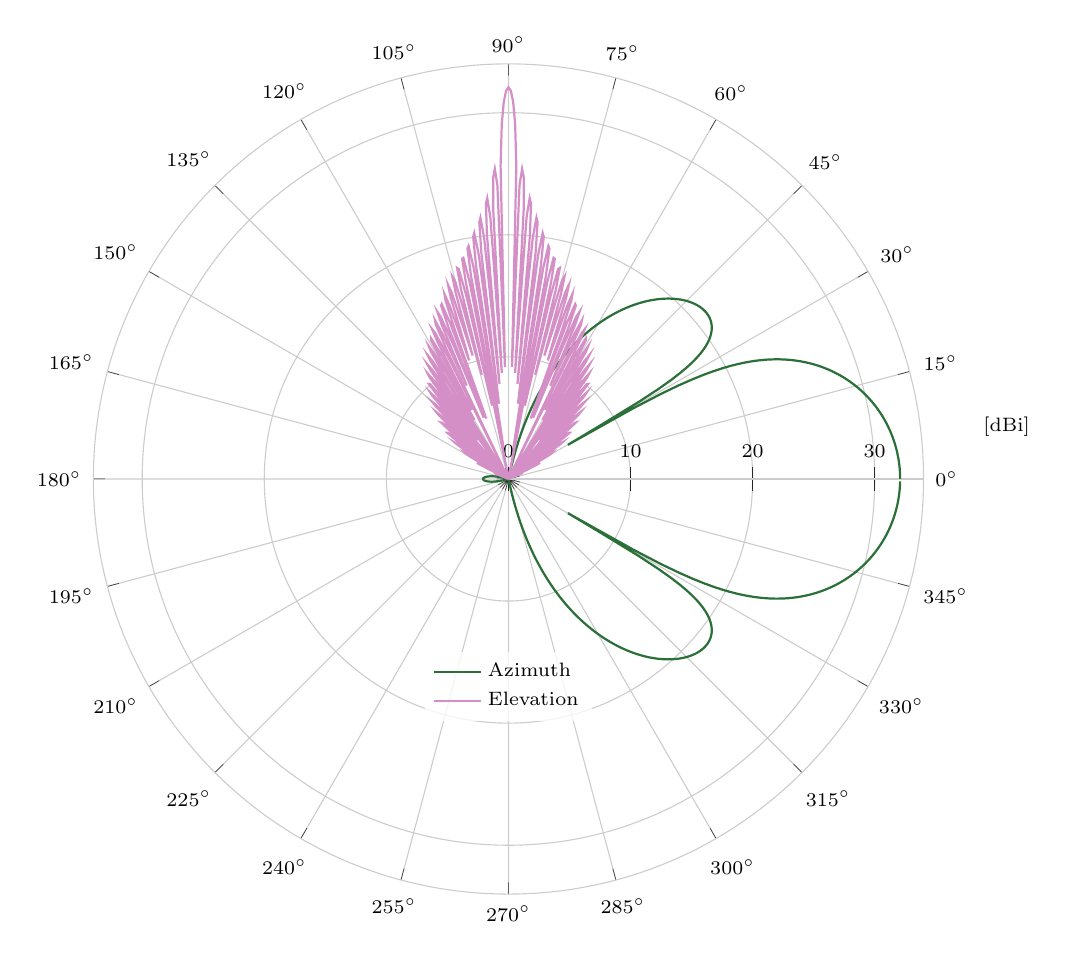
\begin{tikzpicture}

% \definecolor{color0}{rgb}{0.298039215686275,0.447058823529412,0.690196078431373}
% \definecolor{color1}{rgb}{0.866666666666667,0.517647058823529,0.32156862745098}
\definecolor{color0}{rgb}{0.17004232121058,0.436797596475173,0.223725555555555}
\definecolor{color1}{rgb}{0.82995767878942,0.563202403524827,0.776274444444444}

\begin{polaraxis}[
axis line style={white!80!black},
legend cell align={left},
legend style={fill opacity=0.8, draw opacity=1, text opacity=1, at={(0.5,0.25)}, anchor=center, draw=none},
tick align=outside,
tick pos=both,
x grid style={white!80!black},
xmajorgrids,
xmin=0, xmax=360,
xtick style={color=white!15!black},
xticklabel=$\pgfmathprintnumber{\tick}\si{\degree}$,
xticklabel shift=5pt,
y grid style={white!80!black},
ymajorgrids,
ymin=0, ymax=34,
ytick style={color=white!15!black},
ylabel={[dBi]},
ylabel style={at={(1.1,0.54)},anchor=south},
height=\linewidth,
scale=1
]
\addplot [thick, color0]
table {%
0 32.0823996531185
0.36 32.0809739082108
0.72 32.0766961396992
1.08 32.0695647446547
1.44 32.0595770463103
1.8 32.0467292861984
2.16 32.0310166130781
2.52 32.0124330685824
2.88 31.9909715694992
3.24 31.9666238865757
3.6 31.9393806197139
3.96 31.9092311694026
4.32 31.8761637042016
4.68 31.8401651240716
5.04 31.8012210193077
5.4 31.7593156248046
5.76 31.7144317693465
6.12 31.666550819571
6.48 31.6156526182167
6.84 31.5617154162129
7.2 31.5047157981164
7.56 31.4446286003379
7.92 31.3814268215362
8.28 31.3150815244755
8.64 31.2455617285604
9 31.172834292161
9.36 31.0968637837303
9.72 31.0176123405901
10.08 30.9350395141146
10.44 30.8491020998786
10.8 30.759753951144
11.16 30.6669457738412
11.52 30.5706249009515
11.88 30.4707350439026
12.24 30.3672160182519
12.6 30.2600034405412
12.96 30.1490283927454
13.32 30.0342170501995
13.68 29.915490268263
14.04 29.7927631222302
14.4 29.6659443941223
14.76 29.5349359989522
15.12 29.39963234181
15.48 29.2599195956332
15.84 29.1156748877429
16.2 28.9667653810724
16.56 28.8130472334135
16.92 28.6543644148291
17.28 28.490547359503
17.64 28.3214114235223
18 28.1467551141902
18.36 27.9663580491217
18.72 27.7799785941925
19.08 27.5873511178394
19.44 27.3881827845311
19.8 27.1821497914815
20.16 26.968892928528
20.52 26.7480123097479
20.88 26.519061084317
21.24 26.2815378797992
21.6 26.0348776584941
21.96 25.7784405694447
22.32 25.5114982447258
22.68 25.2332168031197
23.04 24.9426355638303
23.4 24.6386401015924
23.76 24.3199277363593
24.12 23.9849627562475
24.48 23.6319174755143
24.84 23.2585933851465
25.2 22.8623137396055
25.56 22.4397741862461
25.92 21.9868300912141
26.28 21.4981853618642
26.64 20.9669223766456
27 20.3837644739587
27.36 19.7358646889178
27.72 19.0047009758734
28.08 18.1621478308759
28.44 17.162422814878
28.8 15.9232910627083
29.16 14.2728358872677
29.52 11.7392845841514
29.88 5.61378065485574
30.24 8.51744537104187
30.6 12.3884809018641
30.96 14.3195886989095
31.32 15.5907979512054
31.68 16.5246097318973
32.04 17.2525545038469
32.4 17.8413803644537
32.76 18.3296545794014
33.12 18.7416876210785
33.48 19.0937954951247
33.84 19.3974613919393
34.2 19.6610740496712
34.56 19.8909485816704
34.92 20.0919582293645
35.28 20.2679424529406
35.64 20.4219801290478
36 20.5565780593009
36.36 20.6738044621006
36.72 20.7753856575314
37.08 20.8627774894966
37.44 20.9372190140856
37.8 20.9997734887525
38.16 21.051360104415
38.52 21.0927788609781
38.88 21.124730290528
39.24 21.1478312578248
39.6 21.1626277384029
39.96 21.1696052423626
40.32 21.1691973857401
40.68 21.1617929907833
41.04 21.1477420078968
41.4 21.1273604862153
41.76 21.1009347703353
42.12 21.068725063239
42.48 21.0309684667358
42.84 20.9878815885689
43.2 20.9396627880721
43.56 20.8864941187106
43.92 20.8285430151353
44.28 20.7659637638596
44.64 20.6988987898484
45 20.6274797858131
45.36 20.5518287065526
45.72 20.4720586470561
46.08 20.3882746201119
46.44 20.3005742467229
46.8 20.2090483706096
47.16 20.1137816064034
47.52 20.014852829733
47.88 19.9123356162382
48.24 19.8062986355551
48.6 19.696806005491
48.96 19.5839176109008
49.32 19.4676893911769
49.68 19.3481735997589
50.04 19.2254190386285
50.4 19.099471270384
50.76 18.9703728101627
51.12 18.8381632994057
51.48 18.7028796632136
51.84 18.5645562528364
52.2 18.4232249746543
52.56 18.278915406851
52.92 18.1316549048374
53.28 17.9814686963637
53.64 17.8283799671475
54 17.6724099377514
54.36 17.5135779323569
54.72 17.3519014400073
55.08 17.1873961688241
55.44 17.0200760936385
55.8 16.8499534974292
56.16 16.6770390069034
56.52 16.501341622516
56.88 16.3228687431784
57.24 16.1416261858716
57.6 15.9576182003422
57.96 15.7708474790259
58.32 15.5813151623139
58.68 15.3890208392456
59.04 15.1939625436837
59.4 14.9961367459995
59.76 14.7955383402702
60.12 14.5921606269605
60.48 14.385995291037
60.84 14.1770323754351
61.2 13.9652602497692
61.56 13.7506655741521
61.92 13.5332332579543
62.28 13.3129464133087
62.64 13.089786303128
63 12.8637322833696
63.36 12.6347617392453
63.72 12.4028500150299
64.08 12.1679703370814
64.44 11.9300937296354
64.8 11.6891889228838
65.16 11.4452222527906
65.52 11.1981575520318
65.88 10.9479560313763
66.24 10.6945761507458
66.6 10.4379734791025
66.96 10.1781005422154
67.32 9.91490665724569
67.68 9.64833775296592
68.04 9.37833617429089
68.4 9.10484046963534
68.76 8.8277851594393
69.12 8.54710048399512
69.48 8.26271212848096
69.84 7.97454092284159
70.2 7.68250251385523
70.56 7.38650700638079
70.92 7.08645857038247
71.28 6.78225500987254
71.64 6.47378728938334
72 6.1609390129714
72.36 5.84358585004305
72.72 5.52159490146752
73.08 5.19482399847504
73.44 4.86312092570651
73.8 4.52632255844941
74.16 4.18425390252617
74.52 3.83672702343984
74.88 3.48353984917351
75.24 3.12447482840694
75.6 2.75929742275487
75.96 2.38775440783988
76.32 2.00957195342736
76.68 1.6244534472877
77.04 1.23207702067236
77.4 0.832092724975583
77.76 0.424119298920075
78.12 0.00774045291598391
78.48 0
78.84 0
79.2 0
79.56 0
79.92 0
80.28 0
80.64 0
81 0
81.36 0
81.72 0
82.08 0
82.44 0
82.8 0
83.16 0
83.52 0
83.88 0
84.24 0
84.6 0
84.96 0
85.32 0
85.68 0
86.04 0
86.4 0
86.76 0
87.12 0
87.48 0
87.84 0
88.2 0
88.56 0
88.92 0
89.28 0
89.64 0
90 0
90.36 0
90.72 0
91.08 0
91.44 0
91.8 0
92.16 0
92.52 0
92.88 0
93.24 0
93.6 0
93.96 0
94.32 0
94.68 0
95.04 0
95.4 0
95.76 0
96.12 0
96.48 0
96.84 0
97.2 0
97.56 0
97.92 0
98.28 0
98.64 0
99 0
99.36 0
99.72 0
100.08 0
100.44 0
100.8 0
101.16 0
101.52 0
101.88 0
102.24 0
102.6 0
102.96 0
103.32 0
103.68 0
104.04 0
104.4 0
104.76 0
105.12 0
105.48 0
105.84 0
106.2 0
106.56 0
106.92 0
107.28 0
107.64 0
108 0
108.36 0
108.72 0
109.08 0
109.44 0
109.8 0
110.16 0
110.52 0
110.88 0
111.24 0
111.6 0
111.96 0
112.32 0
112.68 0
113.04 0
113.4 0
113.76 0
114.12 0
114.48 0
114.84 0
115.2 0
115.56 0
115.92 0
116.28 0
116.64 0
117 0
117.36 0
117.72 0
118.08 0
118.44 0
118.8 0
119.16 0
119.52 0
119.88 0
120.24 0
120.6 0
120.96 0
121.32 0
121.68 0
122.04 0
122.4 0
122.76 0
123.12 0
123.48 0
123.84 0
124.2 0
124.56 0
124.92 0
125.28 0
125.64 0
126 0
126.36 0
126.72 0
127.08 0
127.44 0
127.8 0
128.16 0
128.52 0
128.88 0
129.24 0
129.6 0
129.96 0
130.32 0
130.68 0
131.04 0
131.4 0
131.76 0
132.12 0
132.48 0
132.84 0
133.2 0
133.56 0
133.92 0
134.28 0
134.64 0
135 0
135.36 0
135.72 0
136.08 0
136.44 0
136.8 0
137.16 0
137.52 0
137.88 0
138.24 0
138.6 0
138.96 0
139.32 0
139.68 0
140.04 0
140.4 0
140.76 0
141.12 0
141.48 0
141.84 0
142.2 0
142.56 0
142.92 0
143.28 0
143.64 0
144 0
144.36 0
144.72 0
145.08 0
145.44 0
145.8 0
146.16 0
146.52 0
146.88 0
147.24 0
147.6 0
147.96 0
148.32 0
148.68 0
149.04 0
149.4 0
149.76 0
150.12 0
150.48 0
150.84 0
151.2 0
151.56 0
151.92 0
152.28 0
152.64 0
153 0
153.36 0
153.72 0
154.08 0
154.44 0
154.8 0
155.16 0
155.52 0
155.88 0
156.24 0
156.6 0
156.96 0
157.32 0
157.68 0
158.04 0
158.4 0
158.76 0
159.12 0
159.48 0
159.84 0
160.2 0
160.56 0
160.92 0
161.28 0
161.64 0
162 0
162.36 0
162.72 0
163.08 0
163.44 0
163.8 0
164.16 0
164.52 0
164.88 0.0489513477271579
165.24 0.153703146881245
165.6 0.254895873412252
165.96 0.352635122230193
166.32 0.44701897832222
166.68 0.53813865966697
167.04 0.626079090970205
167.4 0.710919416872603
167.76 0.792733462038832
168.12 0.871590144494323
168.48 0.947553847697097
168.84 1.02068475608968
169.2 1.09103915824458
169.56 1.15866972118043
169.92 1.22362573896665
170.28 1.28595335834155
170.64 1.34569578373033
171 1.40289346375863
171.36 1.45758426110481
171.72 1.50980360731576
172.08 1.55958464402145
172.44 1.60695835181723
172.8 1.65195366793886
173.16 1.69459759372774
173.52 1.73491529277289
173.88 1.77293018051774
174.24 1.80866400603291
174.6 1.84213692657976
174.96 1.87336757552069
175.32 1.90237312407164
175.68 1.92916933733769
176.04 1.95377062502387
176.4 1.97619008716956
176.76 1.99643955521471
177.12 2.01452962867079
177.48 2.03046970763562
177.84 2.04426802136209
178.2 2.0559316530623
178.56 2.06546656110315
178.92 2.0728775967257
179.28 2.07816851839739
179.64 2.08134200288538
180 2.0823996531185
180.36 2.08134200288538
180.72 2.07816851839738
181.08 2.0728775967257
181.44 2.06546656110315
181.8 2.0559316530623
182.16 2.04426802136209
182.52 2.03046970763561
182.88 2.01452962867079
183.24 1.99643955521471
183.6 1.97619008716956
183.96 1.95377062502387
184.32 1.92916933733769
184.68 1.90237312407164
185.04 1.87336757552069
185.4 1.84213692657976
185.76 1.80866400603291
186.12 1.77293018051774
186.48 1.73491529277289
186.84 1.69459759372774
187.2 1.65195366793886
187.56 1.60695835181723
187.92 1.55958464402145
188.28 1.50980360731576
188.64 1.4575842611048
189 1.40289346375863
189.36 1.34569578373032
189.72 1.28595335834155
190.08 1.22362573896665
190.44 1.15866972118042
190.8 1.09103915824457
191.16 1.02068475608968
191.52 0.947553847697097
191.88 0.871590144494323
192.24 0.792733462038832
192.6 0.710919416872592
192.96 0.626079090970205
193.32 0.53813865966697
193.68 0.447018978322205
194.04 0.352635122230179
194.4 0.254895873412252
194.76 0.153703146881245
195.12 0.0489513477271579
195.48 0
195.84 0
196.2 0
196.56 0
196.92 0
197.28 0
197.64 0
198 0
198.36 0
198.72 0
199.08 0
199.44 0
199.8 0
200.16 0
200.52 0
200.88 0
201.24 0
201.6 0
201.96 0
202.32 0
202.68 0
203.04 0
203.4 0
203.76 0
204.12 0
204.48 0
204.84 0
205.2 0
205.56 0
205.92 0
206.28 0
206.64 0
207 0
207.36 0
207.72 0
208.08 0
208.44 0
208.8 0
209.16 0
209.52 0
209.88 0
210.24 0
210.6 0
210.96 0
211.32 0
211.68 0
212.04 0
212.4 0
212.76 0
213.12 0
213.48 0
213.84 0
214.2 0
214.56 0
214.92 0
215.28 0
215.64 0
216 0
216.36 0
216.72 0
217.08 0
217.44 0
217.8 0
218.16 0
218.52 0
218.88 0
219.24 0
219.6 0
219.96 0
220.32 0
220.68 0
221.04 0
221.4 0
221.76 0
222.12 0
222.48 0
222.84 0
223.2 0
223.56 0
223.92 0
224.28 0
224.64 0
225 0
225.36 0
225.72 0
226.08 0
226.44 0
226.8 0
227.16 0
227.52 0
227.88 0
228.24 0
228.6 0
228.96 0
229.32 0
229.68 0
230.04 0
230.4 0
230.76 0
231.12 0
231.48 0
231.84 0
232.2 0
232.56 0
232.92 0
233.28 0
233.64 0
234 0
234.36 0
234.72 0
235.08 0
235.44 0
235.8 0
236.16 0
236.52 0
236.88 0
237.24 0
237.6 0
237.96 0
238.32 0
238.68 0
239.04 0
239.4 0
239.76 0
240.12 0
240.48 0
240.84 0
241.2 0
241.56 0
241.92 0
242.28 0
242.64 0
243 0
243.36 0
243.72 0
244.08 0
244.44 0
244.8 0
245.16 0
245.52 0
245.88 0
246.24 0
246.6 0
246.96 0
247.32 0
247.68 0
248.04 0
248.4 0
248.76 0
249.12 0
249.48 0
249.84 0
250.2 0
250.56 0
250.92 0
251.28 0
251.64 0
252 0
252.36 0
252.72 0
253.08 0
253.44 0
253.8 0
254.16 0
254.52 0
254.88 0
255.24 0
255.6 0
255.96 0
256.32 0
256.68 0
257.04 0
257.4 0
257.76 0
258.12 0
258.48 0
258.84 0
259.2 0
259.56 0
259.92 0
260.28 0
260.64 0
261 0
261.36 0
261.72 0
262.08 0
262.44 0
262.8 0
263.16 0
263.52 0
263.88 0
264.24 0
264.6 0
264.96 0
265.32 0
265.68 0
266.04 0
266.4 0
266.76 0
267.12 0
267.48 0
267.84 0
268.2 0
268.56 0
268.92 0
269.28 0
269.64 0
270 0
270.36 0
270.72 0
271.08 0
271.44 0
271.8 0
272.16 0
272.52 0
272.88 0
273.24 0
273.6 0
273.96 0
274.32 0
274.68 0
275.04 0
275.4 0
275.76 0
276.12 0
276.48 0
276.84 0
277.2 0
277.56 0
277.92 0
278.28 0
278.64 0
279 0
279.36 0
279.72 0
280.08 0
280.44 0
280.8 0
281.16 0
281.52 0
281.88 0.00774045291598391
282.24 0.424119298920015
282.6 0.832092724975595
282.96 1.23207702067236
283.32 1.6244534472878
283.68 2.0095719534274
284.04 2.38775440783994
284.4 2.75929742275487
284.76 3.12447482840694
285.12 3.48353984917351
285.48 3.83672702343979
285.84 4.18425390252624
286.2 4.52632255844941
286.56 4.86312092570661
286.92 5.19482399847517
287.28 5.52159490146753
287.64 5.84358585004305
288 6.1609390129714
288.36 6.47378728938334
288.72 6.78225500987249
289.08 7.08645857038252
289.44 7.38650700638079
289.8 7.68250251385533
290.16 7.97454092284166
290.52 8.262712128481
290.88 8.54710048399512
291.24 8.8277851594393
291.6 9.10484046963534
291.96 9.37833617429086
292.32 9.64833775296598
292.68 9.91490665724569
293.04 10.1781005422155
293.4 10.4379734791026
293.76 10.6945761507458
294.12 10.9479560313763
294.48 11.1981575520318
294.84 11.4452222527906
295.2 11.6891889228837
295.56 11.9300937296354
295.92 12.1679703370814
296.28 12.4028500150299
296.64 12.6347617392454
297 12.8637322833697
297.36 13.089786303128
297.72 13.3129464133087
298.08 13.5332332579543
298.44 13.7506655741521
298.8 13.9652602497693
299.16 14.1770323754351
299.52 14.385995291037
299.88 14.5921606269605
300.24 14.7955383402702
300.6 14.9961367459995
300.96 15.1939625436837
301.32 15.3890208392456
301.68 15.5813151623139
302.04 15.7708474790259
302.4 15.9576182003422
302.76 16.1416261858716
303.12 16.3228687431784
303.48 16.5013416225161
303.84 16.6770390069035
304.2 16.8499534974292
304.56 17.0200760936385
304.92 17.1873961688241
305.28 17.3519014400073
305.64 17.5135779323569
306 17.6724099377514
306.36 17.8283799671476
306.72 17.9814686963637
307.08 18.1316549048374
307.44 18.278915406851
307.8 18.4232249746543
308.16 18.5645562528364
308.52 18.7028796632136
308.88 18.8381632994057
309.24 18.9703728101627
309.6 19.099471270384
309.96 19.2254190386286
310.32 19.3481735997589
310.68 19.4676893911769
311.04 19.5839176109008
311.4 19.696806005491
311.76 19.806298635555
312.12 19.9123356162382
312.48 20.014852829733
312.84 20.1137816064034
313.2 20.2090483706097
313.56 20.3005742467229
313.92 20.3882746201119
314.28 20.4720586470561
314.64 20.5518287065526
315 20.6274797858131
315.36 20.6988987898484
315.72 20.7659637638596
316.08 20.8285430151353
316.44 20.8864941187106
316.8 20.9396627880721
317.16 20.9878815885689
317.52 21.0309684667358
317.88 21.068725063239
318.24 21.1009347703353
318.6 21.1273604862153
318.96 21.1477420078968
319.32 21.1617929907833
319.68 21.1691973857401
320.04 21.1696052423626
320.4 21.1626277384029
320.76 21.1478312578248
321.12 21.124730290528
321.48 21.0927788609781
321.84 21.051360104415
322.2 20.9997734887525
322.56 20.9372190140856
322.92 20.8627774894966
323.28 20.7753856575314
323.64 20.6738044621006
324 20.5565780593009
324.36 20.4219801290478
324.72 20.2679424529406
325.08 20.0919582293645
325.44 19.8909485816704
325.8 19.6610740496711
326.16 19.3974613919392
326.52 19.0937954951246
326.88 18.7416876210785
327.24 18.3296545794014
327.6 17.8413803644537
327.96 17.252554503847
328.32 16.5246097318972
328.68 15.5907979512053
329.04 14.3195886989091
329.4 12.3884809018635
329.76 8.51744537104117
330.12 5.61378065485686
330.48 11.7392845841514
330.84 14.2728358872676
331.2 15.9232910627081
331.56 17.1624228148781
331.92 18.162147830876
332.28 19.0047009758736
332.64 19.7358646889179
333 20.3837644739588
333.36 20.9669223766456
333.72 21.4981853618642
334.08 21.986830091214
334.44 22.439774186246
334.8 22.8623137396056
335.16 23.2585933851465
335.52 23.6319174755143
335.88 23.9849627562475
336.24 24.3199277363593
336.6 24.6386401015924
336.96 24.9426355638303
337.32 25.2332168031197
337.68 25.5114982447258
338.04 25.7784405694447
338.4 26.0348776584941
338.76 26.2815378797992
339.12 26.5190610843171
339.48 26.748012309748
339.84 26.968892928528
340.2 27.1821497914815
340.56 27.3881827845311
340.92 27.5873511178394
341.28 27.7799785941926
341.64 27.9663580491217
342 28.1467551141902
342.36 28.3214114235224
342.72 28.490547359503
343.08 28.6543644148291
343.44 28.8130472334135
343.8 28.9667653810724
344.16 29.1156748877429
344.52 29.2599195956332
344.88 29.39963234181
345.24 29.5349359989522
345.6 29.6659443941223
345.96 29.7927631222302
346.32 29.915490268263
346.68 30.0342170501995
347.04 30.1490283927454
347.4 30.2600034405412
347.76 30.3672160182518
348.12 30.4707350439026
348.48 30.5706249009515
348.84 30.6669457738412
349.2 30.759753951144
349.56 30.8491020998787
349.92 30.9350395141146
350.28 31.0176123405901
350.64 31.0968637837303
351 31.172834292161
351.36 31.2455617285604
351.72 31.3150815244755
352.08 31.3814268215363
352.44 31.444628600338
352.8 31.5047157981164
353.16 31.5617154162129
353.52 31.6156526182167
353.88 31.666550819571
354.24 31.7144317693465
354.6 31.7593156248046
354.96 31.8012210193077
355.32 31.8401651240717
355.68 31.8761637042016
356.04 31.9092311694026
356.4 31.9393806197139
356.76 31.9666238865757
357.12 31.9909715694992
357.48 32.0124330685824
357.84 32.0310166130781
358.2 32.0467292861984
358.56 32.0595770463103
358.92 32.0695647446547
359.28 32.0766961396992
359.64 32.0809739082108
};
\addlegendentry{Azimuth}
\addplot [thick, color1]
table {%
0 0
0.36 0
0.72 0
1.08 0
1.44 0
1.8 0
2.16 0
2.52 0
2.88 0
3.24 0
3.6 0
3.96 0
4.32 0
4.68 0
5.04 0
5.4 0
5.76 0
6.12 0
6.48 0
6.84 0
7.2 0
7.56 0
7.92 0
8.28 0
8.64 0
9 0
9.36 0
9.72 0
10.08 0
10.44 0
10.8 0
11.16 0
11.52 0
11.88 0
12.24 0
12.6 0
12.96 0
13.32 0
13.68 0
14.04 0
14.4 0
14.76 0
15.12 0
15.48 0
15.84 0
16.2 0
16.56 0
16.92 0
17.28 0
17.64 0
18 0
18.36 0
18.72 0
19.08 0
19.44 0
19.8 0
20.16 0
20.52 0
20.88 0
21.24 0
21.6 0
21.96 0.180372156303855
22.32 0.811773368854158
22.68 1.16683273705793
23.04 1.26065380692568
23.4 1.07514733374048
23.76 0.549779911973656
24.12 0
24.48 0
24.84 0
25.2 0
25.56 0
25.92 0.440602477676685
26.28 1.69803057797791
26.64 2.4480533623876
27 2.80846816569756
27.36 2.8062086725232
27.72 2.40242429592901
28.08 1.46044492972236
28.44 0
28.8 0
29.16 0
29.52 0.401472070742081
29.88 2.39542894944444
30.24 3.50657593963374
30.6 4.06282473628139
30.96 4.15459274291373
31.32 3.75834491925156
31.68 2.71250474946848
32.04 0.455920842521515
32.4 0
32.76 0
33.12 2.64976673123414
33.48 4.26738004429774
33.84 5.08286854544635
34.2 5.31535873241986
34.56 4.97961188892434
34.92 3.91158556288321
35.28 1.45652931047097
35.64 0
36 1.29033020476939
36.36 4.26121530681607
36.72 5.67014270620817
37.08 6.27071754788558
37.44 6.22053681594281
37.8 5.44465312007129
38.16 3.4958701418164
38.52 0
38.88 1.28524157045521
39.24 4.95665165728224
39.6 6.54747485802766
39.96 7.19102439554296
40.32 7.0940866972016
40.68 6.15442466718249
41.04 3.71953272343006
41.4 0
41.76 3.75235403885277
42.12 6.55796874423613
42.48 7.76723162462921
42.84 8.06909223597823
43.2 7.53010748445245
43.56 5.79052948266383
43.92 0.3568237327907
44.28 2.98852945060042
44.64 6.85602600863474
45 8.38829571293059
45.36 8.84784952963452
45.72 8.3955024358333
46.08 6.69888458130115
46.44 1.25361063977293
46.8 3.93806827602312
47.16 7.75723253236288
47.52 9.2184880315663
47.88 9.55960996602919
48.24 8.8921609069774
48.6 6.67556047340915
48.96 0
49.32 6.33503604012407
49.68 9.12899985676939
50.04 10.1520778872706
50.4 10.0838851122479
50.76 8.80116301574182
51.12 4.78606870042549
51.48 4.0533629487884
51.84 8.8997887648352
52.2 10.5404191923213
52.56 10.8749508722818
52.92 10.0377391722039
53.28 7.20344384659358
53.64 0.748464167273909
54 8.83731161356657
54.36 10.9471495524085
54.72 11.5144929506098
55.08 10.8667777873431
55.44 8.35945010193549
55.8 0
56.16 9.20785537061138
56.52 11.4969990214747
56.88 12.1106483164636
57.24 11.4433461829526
57.6 8.78732548821111
57.96 1.11596564064463
58.32 10.0953830762302
58.68 12.2108666162489
59.04 12.6761035315309
59.4 11.7754211230517
59.76 8.42135979426715
60.12 5.58975250284818
60.48 11.3467399062714
60.84 13.0154281247106
61.2 13.1454794723433
61.56 11.7453203332115
61.92 6.39973745083512
62.28 9.084124189586
62.64 12.7068464456835
63 13.7764905436317
63.36 13.3790677667577
63.72 11.0193103804751
64.08 0
64.44 11.7577979805518
64.8 13.9491428174411
65.16 14.322759192295
65.52 13.1218303396356
65.88 8.37722196443181
66.24 9.88083720929479
66.6 13.7906018022804
66.96 14.890550582976
67.32 14.4227666649381
67.68 11.7579258388731
68.04 5.40289512150509
68.4 13.3636150795691
68.76 15.2373664283827
69.12 15.3352913773698
69.48 13.6338461827592
69.84 5.27091432220395
70.2 12.6920036531202
70.56 15.4608526618278
70.92 16.0403132384764
71.28 14.9389389102918
71.64 10.2313271780018
72 11.7646753812092
72.36 15.6337075630477
72.72 16.641271400379
73.08 15.9635963417561
73.44 12.5589663515572
73.8 10.5225846325679
74.16 15.8166126039557
74.52 17.2073699910312
74.88 16.8457150389833
75.24 14.1367398136761
75.6 8.80841399878284
75.96 16.063693680144
76.32 17.7901674637806
76.68 17.6677151685172
77.04 15.3825186450394
77.4 6.15685485838583
77.76 16.4245609502051
78.12 18.4321319930227
78.48 18.4888081962142
78.84 16.4739330130783
79.2 0
79.56 16.945561702353
79.92 19.1734894993816
80.28 19.3612357266244
80.64 17.5191478179593
81 2.6117018210888
81.36 17.6736417264379
81.72 20.0612405913771
82.08 20.344230746545
82.44 18.6116389627294
82.8 6.20926538036627
83.16 18.6685236120332
83.52 21.1660480950527
83.88 21.5254694581361
84.24 19.8689986359067
84.6 7.82081743199975
84.96 20.0366131850462
85.32 22.6235945650237
85.68 23.0728889674654
86.04 21.5036686070881
86.4 8.7048290149615
86.76 22.0395018926969
87.12 24.7754311788699
87.48 25.4252954553509
87.84 24.0906196607198
88.2 9.16574122402432
88.56 25.6656187273068
88.92 29.0718317134232
89.28 30.8575524565206
89.64 31.7893679010244
90 32.0823996531185
90.36 31.7893679010243
90.72 30.8575524565206
91.08 29.0718317134231
91.44 25.6656187273068
91.8 9.16574122403036
92.16 24.09061966072
92.52 25.4252954553509
92.88 24.7754311788699
93.24 22.0395018926967
93.6 8.70482901496476
93.96 21.5036686070882
94.32 23.0728889674654
94.68 22.6235945650236
95.04 20.036613185046
95.4 7.8208174320021
95.76 19.8689986359068
96.12 21.5254694581361
96.48 21.1660480950527
96.84 18.668523612033
97.2 6.20926538036914
97.56 18.6116389627294
97.92 20.344230746545
98.28 20.061240591377
98.64 17.6736417264377
99 2.6117018210888
99.36 17.5191478179594
99.72 19.3612357266244
100.08 19.1734894993815
100.44 16.9455617023528
100.8 0
101.16 16.4739330130784
101.52 18.4888081962142
101.88 18.4321319930227
102.24 16.4245609502049
102.6 6.15685485838393
102.96 15.3825186450395
103.32 17.6677151685172
103.68 17.7901674637806
104.04 16.0636936801439
104.4 8.80841399878201
104.76 14.1367398136763
105.12 16.8457150389833
105.48 17.2073699910312
105.84 15.8166126039555
106.2 10.5225846325674
106.56 12.5589663515572
106.92 15.9635963417562
107.28 16.641271400379
107.64 15.6337075630477
108 11.7646753812089
108.36 10.2313271780023
108.72 14.9389389102918
109.08 16.0403132384764
109.44 15.4608526618278
109.8 12.6920036531201
110.16 5.27091432220475
110.52 13.6338461827592
110.88 15.3352913773699
111.24 15.2373664283827
111.6 13.363615079569
111.96 5.40289512150337
112.32 11.7579258388733
112.68 14.4227666649381
113.04 14.890550582976
113.4 13.7906018022805
113.76 9.88083720929422
114.12 8.37722196443181
114.48 13.1218303396357
114.84 14.322759192295
115.2 13.949142817441
115.56 11.7577979805517
115.92 0
116.28 11.0193103804753
116.64 13.3790677667577
117 13.7764905436316
117.36 12.7068464456834
117.72 9.08412418958537
118.08 6.39973745083568
118.44 11.7453203332115
118.8 13.1454794723432
119.16 13.0154281247105
119.52 11.3467399062714
119.88 5.58975250284818
120.24 8.42135979426715
120.6 11.7754211230519
120.96 12.6761035315308
121.32 12.210866616249
121.68 10.0953830762301
122.04 1.11596564064288
122.4 8.78732548821111
122.76 11.4433461829526
123.12 12.1106483164636
123.48 11.4969990214747
123.84 9.20785537061121
124.2 0
124.56 8.35945010193574
124.92 10.8667777873432
125.28 11.5144929506099
125.64 10.9471495524085
126 8.83731161356651
126.36 0.748464167274688
126.72 7.20344384659372
127.08 10.037739172204
127.44 10.8749508722816
127.8 10.5404191923213
128.16 8.89978876483508
128.52 4.05336294878797
128.88 4.78606870042541
129.24 8.80116301574211
129.6 10.0838851122479
129.96 10.1520778872706
130.32 9.12899985676916
130.68 6.33503604012378
131.04 0
131.4 6.67556047340932
131.76 8.89216090697731
132.12 9.55960996602919
132.48 9.2184880315663
132.84 7.757232532363
133.2 3.93806827602296
133.56 1.25361063977319
133.92 6.69888458130122
134.28 8.39550243583318
134.64 8.84784952963453
135 8.38829571293053
135.36 6.85602600863474
135.72 2.98852945060042
136.08 0.356823732789158
136.44 5.79052948266383
136.8 7.53010748445272
137.16 8.06909223597819
137.52 7.76723162462921
137.88 6.55796874423634
138.24 3.75235403885277
138.6 0
138.96 3.71953272342997
139.32 6.15442466718248
139.68 7.09408669720158
140.04 7.19102439554301
140.4 6.54747485802791
140.76 4.95665165728271
141.12 1.28524157045521
141.48 0
141.84 3.4958701418164
142.2 5.4446531200714
142.56 6.22053681594281
142.92 6.27071754788554
143.28 5.67014270620805
143.64 4.26121530681608
144 1.29033020477023
144.36 0
144.72 1.45652931047097
145.08 3.91158556288345
145.44 4.97961188892434
145.8 5.31535873241986
146.16 5.08286854544643
146.52 4.26738004429741
146.88 2.64976673123414
147.24 0
147.6 0
147.96 0.45592084252151
148.32 2.71250474946841
148.68 3.75834491925143
149.04 4.15459274291377
149.4 4.06282473628167
149.76 3.50657593963374
150.12 2.39542894944444
150.48 0.401472070742082
150.84 0
151.2 0
151.56 0
151.92 1.4604449297227
152.28 2.40242429592911
152.64 2.80620867252321
153 2.80846816569758
153.36 2.44805336238759
153.72 1.69803057797791
154.08 0.44060247767668
154.44 0
154.8 0
155.16 0
155.52 0
155.88 0
156.24 0.549779911973652
156.6 1.07514733374048
156.96 1.26065380692567
157.32 1.1668327370577
157.68 0.81177336885418
158.04 0.180372156303893
158.4 0
158.76 0
159.12 0
159.48 0
159.84 0
160.2 0
160.56 0
160.92 0
161.28 0
161.64 0
162 0
162.36 0
162.72 0
163.08 0
163.44 0
163.8 0
164.16 0
164.52 0
164.88 0
165.24 0
165.6 0
165.96 0
166.32 0
166.68 0
167.04 0
167.4 0
167.76 0
168.12 0
168.48 0
168.84 0
169.2 0
169.56 0
169.92 0
170.28 0
170.64 0
171 0
171.36 0
171.72 0
172.08 0
172.44 0
172.8 0
173.16 0
173.52 0
173.88 0
174.24 0
174.6 0
174.96 0
175.32 0
175.68 0
176.04 0
176.4 0
176.76 0
177.12 0
177.48 0
177.84 0
178.2 0
178.56 0
178.92 0
179.28 0
179.64 0
};
\addlegendentry{Elevation}
\end{polaraxis}

\end{tikzpicture}

\caption{64 by 4 antenna array}
\end{subfigure}~
\begin{subfigure}[t]{0.5\linewidth}
% This file was created by tikzplotlib v0.9.3.
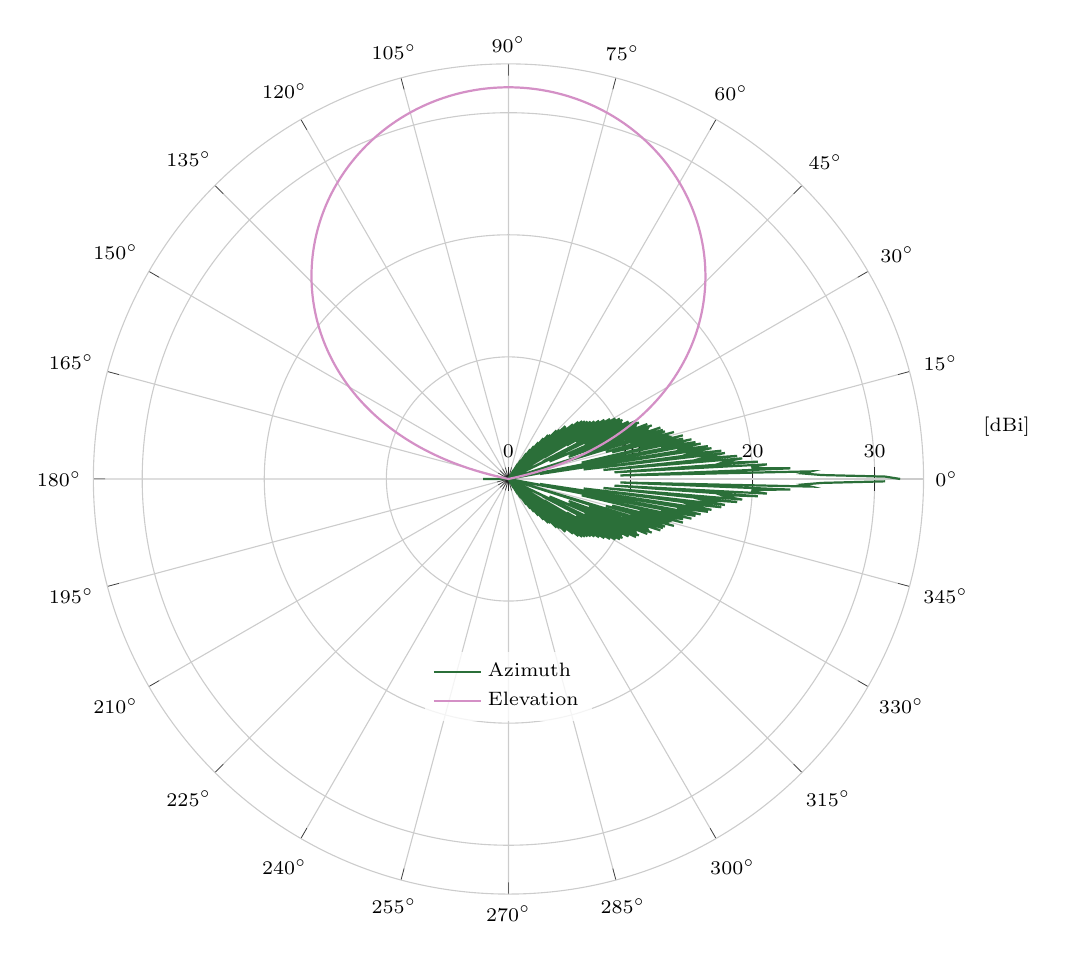
\begin{tikzpicture}

% \definecolor{color0}{rgb}{0.298039215686275,0.447058823529412,0.690196078431373}
% \definecolor{color1}{rgb}{0.866666666666667,0.517647058823529,0.32156862745098}
\definecolor{color0}{rgb}{0.17004232121058,0.436797596475173,0.223725555555555}
\definecolor{color1}{rgb}{0.82995767878942,0.563202403524827,0.776274444444444}

\begin{polaraxis}[
axis line style={white!80!black},
legend cell align={left},
legend style={fill opacity=0.8, draw opacity=1, text opacity=1, at={(0.5,0.25)}, anchor=center, draw=none},
tick align=outside,
tick pos=both,
x grid style={white!80!black},
xmajorgrids,
xmin=0, xmax=360,
xtick style={color=white!15!black},
xticklabel=$\pgfmathprintnumber{\tick}\si{\degree}$,
xticklabel shift=5pt,
y grid style={white!80!black},
ymajorgrids,
ymin=0, ymax=34,
ytick style={color=white!15!black},
ylabel={[dBi]},
ylabel style={at={(1.1,0.54)},anchor=south},
height=\linewidth,
scale=1
]
\addplot [thick, color0]
table {%
0 32.0823996531185
0.36 30.8583938964034
0.72 25.6676209363605
1.08 24.101747695479
1.44 24.785898647833
1.8 9.16517404006753
2.16 23.1086442923984
2.52 20.0205765053258
2.88 19.9904843734441
3.24 21.2018728052587
3.6 8.70297647991541
3.96 20.481629332569
4.32 17.5072364782187
4.68 17.9561733939178
5.04 19.223525218836
5.4 7.81799921868414
5.76 18.8293690730808
6.12 15.9075809219244
6.48 16.5175402743549
6.84 17.8542474512016
7.2 6.20682794704847
7.56 17.5881322314126
7.92 14.8333718725555
8.28 15.2966442386463
8.64 16.823089018355
9 2.61095501637061
9.36 16.5545791429612
9.72 14.1473048535403
10.08 14.1041762781489
10.44 16.0110402261541
10.8 0
11.16 15.6157845282792
11.52 13.7600870812849
11.88 12.7738806415631
12.24 15.3394379605719
12.6 6.14877031668849
12.96 14.6761791932699
13.32 13.5787912573604
13.68 11.0516526866612
14.04 14.7310620572231
14.4 8.77063668898148
14.76 13.6168423284775
15.12 13.4974684778605
15.48 8.28030550378581
15.84 14.088762396073
16.2 10.4096273672511
16.56 12.2394127582323
16.92 13.397533547869
17.28 0
17.64 13.2714571200642
18 11.4928170690826
18.36 10.0942032193084
18.72 13.139974450182
19.08 6.97570572911849
19.44 12.0373513181223
19.8 12.1156612837643
20.16 5.25339302208833
20.52 12.5340972067819
20.88 10.0113640458377
21.24 9.82318138869628
21.6 12.2312545807428
21.96 5.37907862781411
22.32 11.2361257758137
22.68 11.2834260318945
23.04 3.65233403354113
23.4 11.6421614238486
23.76 9.6307302334347
24.12 8.24966695879438
24.48 11.4755935885603
24.84 6.84907513582404
25.2 9.77547456647385
25.56 10.9013244224703
25.92 0
26.28 10.3819659186875
26.64 9.99573848458596
27 3.16667726099058
27.36 10.5195232884917
27.72 8.79344834804319
28.08 6.31540673096002
28.44 10.3772394090719
28.8 7.30330523717347
29.16 7.56435484117399
29.52 10.0649325948429
29.88 5.51706140290302
30.24 8.12665724573575
30.6 9.66120891490653
30.96 3.4277085704631
31.32 8.32909086811158
31.68 9.22933971015149
32.04 1.10397545380035
32.4 8.31042414200247
32.76 8.82091532373352
33.12 0
33.48 8.13817292553694
33.84 8.47313770710793
34.2 0
34.56 7.83995594944998
34.92 8.20336812591057
35.28 0
35.64 7.41144953091491
36 8.00468121296023
36.36 0.730932779386274
36.72 6.81301302578548
37.08 7.84499856843154
37.44 2.48045403246668
37.8 5.95204252810382
38.16 7.66909271434248
38.52 3.94506421598444
38.88 4.62512675212385
39.24 7.39928115076371
39.6 5.08453773552872
39.96 2.27129765080333
40.32 6.92788560359433
40.68 5.89216625305273
41.04 0
41.4 6.08716295829
41.76 6.34200485287727
42.12 0.325619377475098
42.48 4.54167536301775
42.84 6.36511638819107
43.2 3.74383046312892
43.56 1.19620264313543
43.92 5.80882123459219
44.28 5.19149786094495
44.64 0
45 4.29546109067566
45.36 5.59692915180559
45.72 2.81244116035106
46.08 0.303263038262509
46.44 4.97616783266221
46.8 4.66620170634348
47.16 0
47.52 2.6846418578574
47.88 4.84922121418238
48.24 3.38030825797021
48.6 0
48.96 3.31017783690241
49.32 4.39563427548122
49.68 2.07040865518899
50.04 0
50.4 3.28577323489
50.76 3.87010449158014
51.12 1.11241360457345
51.48 0
51.84 2.91316449214345
52.2 3.40581349290922
52.56 0.78335165765696
52.92 0
53.28 2.24445119518649
53.64 3.01069411219693
54 1.01847189264471
54.36 0
54.72 1.1246841079576
55.08 2.55821444969545
55.44 1.46761743146484
55.8 0
56.16 0
56.52 1.77560621933272
56.88 1.73821139755354
57.24 0
57.6 0
57.96 0.108140364928579
58.32 1.44170027398225
58.68 0.66319179585816
59.04 0
59.4 0
59.76 0
60.12 0.838681034720221
60.48 0
60.84 0
61.2 0
61.56 0
61.92 0.171352565936958
62.28 0
62.64 0
63 0
63.36 0
63.72 0
64.08 0
64.44 0
64.8 0
65.16 0
65.52 0
65.88 0
66.24 0
66.6 0
66.96 0
67.32 0
67.68 0
68.04 0
68.4 0
68.76 0
69.12 0
69.48 0
69.84 0
70.2 0
70.56 0
70.92 0
71.28 0
71.64 0
72 0
72.36 0
72.72 0
73.08 0
73.44 0
73.8 0
74.16 0
74.52 0
74.88 0
75.24 0
75.6 0
75.96 0
76.32 0
76.68 0
77.04 0
77.4 0
77.76 0
78.12 0
78.48 0
78.84 0
79.2 0
79.56 0
79.92 0
80.28 0
80.64 0
81 0
81.36 0
81.72 0
82.08 0
82.44 0
82.8 0
83.16 0
83.52 0
83.88 0
84.24 0
84.6 0
84.96 0
85.32 0
85.68 0
86.04 0
86.4 0
86.76 0
87.12 0
87.48 0
87.84 0
88.2 0
88.56 0
88.92 0
89.28 0
89.64 0
90 0
90.36 0
90.72 0
91.08 0
91.44 0
91.8 0
92.16 0
92.52 0
92.88 0
93.24 0
93.6 0
93.96 0
94.32 0
94.68 0
95.04 0
95.4 0
95.76 0
96.12 0
96.48 0
96.84 0
97.2 0
97.56 0
97.92 0
98.28 0
98.64 0
99 0
99.36 0
99.72 0
100.08 0
100.44 0
100.8 0
101.16 0
101.52 0
101.88 0
102.24 0
102.6 0
102.96 0
103.32 0
103.68 0
104.04 0
104.4 0
104.76 0
105.12 0
105.48 0
105.84 0
106.2 0
106.56 0
106.92 0
107.28 0
107.64 0
108 0
108.36 0
108.72 0
109.08 0
109.44 0
109.8 0
110.16 0
110.52 0
110.88 0
111.24 0
111.6 0
111.96 0
112.32 0
112.68 0
113.04 0
113.4 0
113.76 0
114.12 0
114.48 0
114.84 0
115.2 0
115.56 0
115.92 0
116.28 0
116.64 0
117 0
117.36 0
117.72 0
118.08 0
118.44 0
118.8 0
119.16 0
119.52 0
119.88 0
120.24 0
120.6 0
120.96 0
121.32 0
121.68 0
122.04 0
122.4 0
122.76 0
123.12 0
123.48 0
123.84 0
124.2 0
124.56 0
124.92 0
125.28 0
125.64 0
126 0
126.36 0
126.72 0
127.08 0
127.44 0
127.8 0
128.16 0
128.52 0
128.88 0
129.24 0
129.6 0
129.96 0
130.32 0
130.68 0
131.04 0
131.4 0
131.76 0
132.12 0
132.48 0
132.84 0
133.2 0
133.56 0
133.92 0
134.28 0
134.64 0
135 0
135.36 0
135.72 0
136.08 0
136.44 0
136.8 0
137.16 0
137.52 0
137.88 0
138.24 0
138.6 0
138.96 0
139.32 0
139.68 0
140.04 0
140.4 0
140.76 0
141.12 0
141.48 0
141.84 0
142.2 0
142.56 0
142.92 0
143.28 0
143.64 0
144 0
144.36 0
144.72 0
145.08 0
145.44 0
145.8 0
146.16 0
146.52 0
146.88 0
147.24 0
147.6 0
147.96 0
148.32 0
148.68 0
149.04 0
149.4 0
149.76 0
150.12 0
150.48 0
150.84 0
151.2 0
151.56 0
151.92 0
152.28 0
152.64 0
153 0
153.36 0
153.72 0
154.08 0
154.44 0
154.8 0
155.16 0
155.52 0
155.88 0
156.24 0
156.6 0
156.96 0
157.32 0
157.68 0
158.04 0
158.4 0
158.76 0
159.12 0
159.48 0
159.84 0
160.2 0
160.56 0
160.92 0
161.28 0
161.64 0
162 0
162.36 0
162.72 0
163.08 0
163.44 0
163.8 0
164.16 0
164.52 0
164.88 0
165.24 0
165.6 0
165.96 0
166.32 0
166.68 0
167.04 0
167.4 0
167.76 0
168.12 0
168.48 0
168.84 0
169.2 0
169.56 0
169.92 0
170.28 0
170.64 0
171 0
171.36 0
171.72 0
172.08 0
172.44 0
172.8 0
173.16 0
173.52 0
173.88 0
174.24 0
174.6 0
174.96 0
175.32 0
175.68 0
176.04 0
176.4 0
176.76 0
177.12 0
177.48 0
177.84 0
178.2 0
178.56 0
178.92 0
179.28 0
179.64 0.858761991078055
180 2.0823996531185
180.36 0.858761991078055
180.72 0
181.08 0
181.44 0
181.8 0
182.16 0
182.52 0
182.88 0
183.24 0
183.6 0
183.96 0
184.32 0
184.68 0
185.04 0
185.4 0
185.76 0
186.12 0
186.48 0
186.84 0
187.2 0
187.56 0
187.92 0
188.28 0
188.64 0
189 0
189.36 0
189.72 0
190.08 0
190.44 0
190.8 0
191.16 0
191.52 0
191.88 0
192.24 0
192.6 0
192.96 0
193.32 0
193.68 0
194.04 0
194.4 0
194.76 0
195.12 0
195.48 0
195.84 0
196.2 0
196.56 0
196.92 0
197.28 0
197.64 0
198 0
198.36 0
198.72 0
199.08 0
199.44 0
199.8 0
200.16 0
200.52 0
200.88 0
201.24 0
201.6 0
201.96 0
202.32 0
202.68 0
203.04 0
203.4 0
203.76 0
204.12 0
204.48 0
204.84 0
205.2 0
205.56 0
205.92 0
206.28 0
206.64 0
207 0
207.36 0
207.72 0
208.08 0
208.44 0
208.8 0
209.16 0
209.52 0
209.88 0
210.24 0
210.6 0
210.96 0
211.32 0
211.68 0
212.04 0
212.4 0
212.76 0
213.12 0
213.48 0
213.84 0
214.2 0
214.56 0
214.92 0
215.28 0
215.64 0
216 0
216.36 0
216.72 0
217.08 0
217.44 0
217.8 0
218.16 0
218.52 0
218.88 0
219.24 0
219.6 0
219.96 0
220.32 0
220.68 0
221.04 0
221.4 0
221.76 0
222.12 0
222.48 0
222.84 0
223.2 0
223.56 0
223.92 0
224.28 0
224.64 0
225 0
225.36 0
225.72 0
226.08 0
226.44 0
226.8 0
227.16 0
227.52 0
227.88 0
228.24 0
228.6 0
228.96 0
229.32 0
229.68 0
230.04 0
230.4 0
230.76 0
231.12 0
231.48 0
231.84 0
232.2 0
232.56 0
232.92 0
233.28 0
233.64 0
234 0
234.36 0
234.72 0
235.08 0
235.44 0
235.8 0
236.16 0
236.52 0
236.88 0
237.24 0
237.6 0
237.96 0
238.32 0
238.68 0
239.04 0
239.4 0
239.76 0
240.12 0
240.48 0
240.84 0
241.2 0
241.56 0
241.92 0
242.28 0
242.64 0
243 0
243.36 0
243.72 0
244.08 0
244.44 0
244.8 0
245.16 0
245.52 0
245.88 0
246.24 0
246.6 0
246.96 0
247.32 0
247.68 0
248.04 0
248.4 0
248.76 0
249.12 0
249.48 0
249.84 0
250.2 0
250.56 0
250.92 0
251.28 0
251.64 0
252 0
252.36 0
252.72 0
253.08 0
253.44 0
253.8 0
254.16 0
254.52 0
254.88 0
255.24 0
255.6 0
255.96 0
256.32 0
256.68 0
257.04 0
257.4 0
257.76 0
258.12 0
258.48 0
258.84 0
259.2 0
259.56 0
259.92 0
260.28 0
260.64 0
261 0
261.36 0
261.72 0
262.08 0
262.44 0
262.8 0
263.16 0
263.52 0
263.88 0
264.24 0
264.6 0
264.96 0
265.32 0
265.68 0
266.04 0
266.4 0
266.76 0
267.12 0
267.48 0
267.84 0
268.2 0
268.56 0
268.92 0
269.28 0
269.64 0
270 0
270.36 0
270.72 0
271.08 0
271.44 0
271.8 0
272.16 0
272.52 0
272.88 0
273.24 0
273.6 0
273.96 0
274.32 0
274.68 0
275.04 0
275.4 0
275.76 0
276.12 0
276.48 0
276.84 0
277.2 0
277.56 0
277.92 0
278.28 0
278.64 0
279 0
279.36 0
279.72 0
280.08 0
280.44 0
280.8 0
281.16 0
281.52 0
281.88 0
282.24 0
282.6 0
282.96 0
283.32 0
283.68 0
284.04 0
284.4 0
284.76 0
285.12 0
285.48 0
285.84 0
286.2 0
286.56 0
286.92 0
287.28 0
287.64 0
288 0
288.36 0
288.72 0
289.08 0
289.44 0
289.8 0
290.16 0
290.52 0
290.88 0
291.24 0
291.6 0
291.96 0
292.32 0
292.68 0
293.04 0
293.4 0
293.76 0
294.12 0
294.48 0
294.84 0
295.2 0
295.56 0
295.92 0
296.28 0
296.64 0
297 0
297.36 0
297.72 0
298.08 0.171352565936958
298.44 0
298.8 0
299.16 0
299.52 0
299.88 0.838681034719746
300.24 0
300.6 0
300.96 0
301.32 0.66319179585816
301.68 1.44170027398222
302.04 0.108140364928197
302.4 0
302.76 0
303.12 1.73821139755371
303.48 1.77560621933267
303.84 0
304.2 0
304.56 1.46761743146484
304.92 2.55821444969643
305.28 1.1246841079579
305.64 0
306 1.01847189264471
306.36 3.01069411219678
306.72 2.24445119518622
307.08 0
307.44 0.78335165765696
307.8 3.40581349290922
308.16 2.91316449214381
308.52 0
308.88 1.11241360457345
309.24 3.87010449158014
309.6 3.28577323488937
309.96 0
310.32 2.07040865518968
310.68 4.39563427548122
311.04 3.31017783690241
311.4 0
311.76 3.38030825797018
312.12 4.84922121418214
312.48 2.6846418578574
312.84 0
313.2 4.66620170634373
313.56 4.97616783266199
313.92 0.303263038261389
314.28 2.81244116035106
314.64 5.59692915180583
315 4.29546109067558
315.36 0
315.72 5.19149786094495
316.08 5.80882123459195
316.44 1.19620264313306
316.8 3.74383046312973
317.16 6.36511638819117
317.52 4.54167536301775
317.88 0.325619377473282
318.24 6.34200485287663
318.6 6.08716295828983
318.96 0
319.32 5.89216625305402
319.68 6.92788560359449
320.04 2.27129765080263
320.4 5.08453773552907
320.76 7.39928115076371
321.12 4.6251267521243
321.48 3.94506421598429
321.84 7.66909271434288
322.2 5.95204252810382
322.56 2.4804540324692
322.92 7.84499856843172
323.28 6.81301302578502
323.64 0.730932779387522
324 8.00468121296023
324.36 7.4114495309151
324.72 0
325.08 8.2033681259109
325.44 7.83995594944998
325.8 0
326.16 8.47313770710826
326.52 8.13817292553667
326.88 0
327.24 8.82091532373352
327.6 8.31042414200284
327.96 1.10397545379715
328.32 9.22933971015168
328.68 8.32909086811111
329.04 3.42770857046782
329.4 9.66120891490691
329.76 8.12665724573492
330.12 5.51706140290361
330.48 10.0649325948429
330.84 7.56435484117487
331.2 7.30330523717216
331.56 10.377239409072
331.92 6.31540673095914
332.28 8.79344834804525
332.64 10.5195232884914
333 3.16667726098824
333.36 9.99573848458602
333.72 10.3819659186875
334.08 0
334.44 10.90132442247
334.8 9.77547456647305
335.16 6.84907513582502
335.52 11.4755935885603
335.88 8.24966695879244
336.24 9.63073023343532
336.6 11.6421614238484
336.96 3.65233403354113
337.32 11.2834260318945
337.68 11.2361257758139
338.04 5.37907862781796
338.4 12.2312545807429
338.76 9.82318138869628
339.12 10.0113640458394
339.48 12.5340972067818
339.84 5.25339302208579
340.2 12.1156612837643
340.56 12.0373513181223
340.92 6.97570572911726
341.28 13.1399744501821
341.64 10.0942032193079
342 11.4928170690826
342.36 13.2714571200638
342.72 0
343.08 13.3975335478691
343.44 12.2394127582323
343.8 10.4096273672511
344.16 14.088762396073
344.52 8.28030550378852
344.88 13.4974684778608
345.24 13.6168423284775
345.6 8.77063668898569
345.96 14.7310620572231
346.32 11.0516526866596
346.68 13.5787912573609
347.04 14.6761791932699
347.4 6.14877031668529
347.76 15.3394379605717
348.12 12.7738806415625
348.48 13.7600870812849
348.84 15.6157845282788
349.2 0
349.56 16.0110402261544
349.92 14.1041762781484
350.28 14.1473048535403
350.64 16.5545791429613
351 2.6109550163908
351.36 16.8230890183552
351.72 15.2966442386463
352.08 14.8333718725573
352.44 17.5881322314125
352.8 6.20682794703761
353.16 17.8542474512018
353.52 16.5175402743549
353.88 15.9075809219238
354.24 18.8293690730809
354.6 7.81799921867874
354.96 19.223525218836
355.32 17.9561733939164
355.68 17.5072364782206
356.04 20.4816293325689
356.4 8.7029764799087
356.76 21.2018728052587
357.12 19.9904843734445
357.48 20.0205765053245
357.84 23.1086442923984
358.2 9.16517404006753
358.56 24.7858986478339
358.92 24.1017476954777
359.28 25.6676209363619
359.64 30.8583938964036
};
\addlegendentry{Azimuth}
\addplot [thick, color1]
table {%
0 0
0.36 0
0.72 0
1.08 0
1.44 0
1.8 0
2.16 0
2.52 0
2.88 0
3.24 0
3.6 0
3.96 0
4.32 0
4.68 0
5.04 0
5.4 0
5.76 0
6.12 0
6.48 0
6.84 0
7.2 0
7.56 0
7.92 0
8.28 0
8.64 0
9 0
9.36 0
9.72 0
10.08 0
10.44 0
10.8 0
11.16 0
11.52 0
11.88 0.0175802091407462
12.24 0.435203238003078
12.6 0.844534965692109
12.96 1.24599841342142
13.32 1.6399817636888
13.68 2.02684207608983
14.04 2.40690852039994
14.4 2.7804852002814
14.76 3.14785362828727
15.12 3.50927490259583
15.48 3.86499162759893
15.84 4.21522961368695
16.2 4.56019938601123
16.56 4.90009752742156
16.92 5.23510787698197
17.28 5.56540260231277
17.64 5.89114316137228
18 6.21248116708316
18.36 6.52955916634949
18.72 6.842511343441
19.08 7.15146415639034
19.44 7.45653691391756
19.8 7.7578422994311
20.16 8.0554868478276
20.52 8.3495713801045
20.88 8.64019140018814
21.24 8.92743745785396
21.6 9.21139548115824
21.96 9.49214708140604
22.32 9.769769833335
22.68 10.0443375328949
23.04 10.3159204347402
23.4 10.5845854713227
23.76 10.8503964552712
24.12 11.113414266565
24.48 11.3736970258538
24.84 11.6313002551378
25.2 11.8862770268989
25.56 12.1386781026666
25.92 12.3885520619043
26.28 12.6359454220189
26.64 12.8809027502162
27 13.1234667678609
27.36 13.3636784479358
27.72 13.6015771061413
28.08 13.8372004861292
28.44 14.0705848393166
28.8 14.3017649996914
29.16 14.5307744539813
29.52 14.757645407528
29.88 14.9824088461791
30.24 15.2050945944835
30.6 15.4257313704532
30.96 15.6443468371322
31.32 15.8609676511934
31.68 16.0756195087688
32.04 16.2883271886986
32.4 16.4991145933733
32.76 16.7080047873288
33.12 16.9150200337405
33.48 17.1201818289535
33.84 17.3235109351746
34.2 17.5250274114429
34.56 17.7247506429872
34.92 17.9226993690695
35.28 18.1188917094097
35.64 18.3133451892753
36 18.5060767633185
36.36 18.6971028382349
36.72 18.8864392943127
37.08 19.0741015059383
37.44 19.2601043611179
37.8 19.4444622800719
38.16 19.6271892329549
38.52 19.8082987567502
38.88 19.9878039713844
39.24 20.1657175951067
39.6 20.3420519591707
39.96 20.5168190218589
40.32 20.6900303818835
40.68 20.8616972911975
41.04 21.0318306672469
41.4 21.2004411046933
41.76 21.3675388866344
42.12 21.5331339953478
42.48 21.6972361225825
42.84 21.8598546794218
43.2 22.0209988057374
43.56 22.1806773792562
43.92 22.3388990242583
44.28 22.4956721199247
44.64 22.6510048083506
45 22.8049050022417
45.36 22.9573803923073
45.72 23.1084384543652
46.08 23.2580864561718
46.44 23.40633146399
46.8 23.553180348907
47.16 23.6986397929132
47.52 23.8427162947534
47.88 23.9854161755605
48.24 24.1267455842808
48.6 24.2667105029007
48.96 24.4053167514838
49.32 24.5425699930252
49.68 24.6784757381324
50.04 24.8130393495401
50.4 24.9462660464646
50.76 25.0781609088059
51.12 25.208728881204
51.48 25.3379747769536
51.84 25.4659032817857
52.2 25.5925189575193
52.56 25.7178262455896
52.92 25.8418294704572
53.28 25.9645328429037
53.64 26.0859404632171
54 26.2060563242725
54.36 26.3248843145114
54.72 26.4424282208239
55.08 26.5586917313372
55.44 26.6736784381146
55.8 26.7873918397674
56.16 26.8998353439839
56.52 27.0110122699785
56.88 27.1209258508628
57.24 27.2295792359431
57.6 27.3369754929461
57.96 27.4431176101748
58.32 27.548008498599
58.68 27.6516509938805
59.04 27.7540478583371
59.4 27.8552017828465
59.76 27.9551153886922
60.12 28.0537912293544
60.48 28.1512317922465
60.84 28.2474395003996
61.2 28.3424167140976
61.56 28.4361657324623
61.92 28.5286887949931
62.28 28.6199880830603
62.64 28.7100657213545
63 28.7989237792943
63.36 28.886564272392
63.72 28.97298916358
64.08 29.0582003644982
64.44 29.1421997367447
64.8 29.2249890930892
65.16 29.3065701986529
65.52 29.3869447720526
65.88 29.4661144865134
66.24 29.5440809709481
66.6 29.6208458110064
66.96 29.6964105500936
67.32 29.7707766903602
67.68 29.8439456936628
68.04 29.9159189824976
68.4 29.9866979409071
68.76 30.0562839153604
69.12 30.1246782156088
69.48 30.1918821155159
69.84 30.2578968538641
70.2 30.3227236351383
70.56 30.3863636302854
70.92 30.4488179774534
71.28 30.5100877827075
71.64 30.5701741207261
72 30.6290780354761
72.36 30.6868005408675
72.72 30.7433426213898
73.08 30.7987052327284
73.44 30.8528893023627
73.8 30.9058957301465
74.16 30.9577253888697
74.52 31.008379124804
74.88 31.0578577582307
75.24 31.1061620839525
75.6 31.1532928717889
75.96 31.1992508670556
76.32 31.2440367910294
76.68 31.2876513413963
77.04 31.3300951926864
77.4 31.3713689966932
77.76 31.4114733828789
78.12 31.450408958766
78.48 31.4881763103146
78.84 31.524776002287
79.2 31.560208578598
79.56 31.5944745626534
79.92 31.6275744576746
80.28 31.6595087470117
80.64 31.6902778944432
81 31.7198823444641
81.36 31.7483225225621
81.72 31.7755988354816
82.08 31.8017116714765
82.44 31.8266614005509
82.8 31.8504483746892
83.16 31.8730729280745
83.52 31.894535377296
83.88 31.9148360215458
84.24 31.9339751428045
84.6 31.9519530060165
84.96 31.9687698592544
85.32 31.9844259338731
85.68 31.9989214446534
86.04 32.0122565899356
86.4 32.0244315517427
86.76 32.0354464958931
87.12 32.0453015721041
87.48 32.0539969140846
87.84 32.0615326396183
88.2 32.0679088506367
88.56 32.0731256332827
88.92 32.077183057964
89.28 32.0800811793968
89.64 32.0818200366398
90 32.0823996531185
90.36 32.0818200366398
90.72 32.0800811793968
91.08 32.077183057964
91.44 32.0731256332827
91.8 32.0679088506367
92.16 32.0615326396183
92.52 32.0539969140846
92.88 32.0453015721041
93.24 32.0354464958931
93.6 32.0244315517427
93.96 32.0122565899356
94.32 31.9989214446534
94.68 31.9844259338731
95.04 31.9687698592544
95.4 31.9519530060165
95.76 31.9339751428045
96.12 31.9148360215458
96.48 31.894535377296
96.84 31.8730729280745
97.2 31.8504483746892
97.56 31.8266614005509
97.92 31.8017116714765
98.28 31.7755988354816
98.64 31.7483225225621
99 31.7198823444641
99.36 31.6902778944432
99.72 31.6595087470117
100.08 31.6275744576746
100.44 31.5944745626534
100.8 31.560208578598
101.16 31.524776002287
101.52 31.4881763103146
101.88 31.450408958766
102.24 31.4114733828789
102.6 31.3713689966932
102.96 31.3300951926864
103.32 31.2876513413963
103.68 31.2440367910294
104.04 31.1992508670556
104.4 31.1532928717889
104.76 31.1061620839525
105.12 31.0578577582307
105.48 31.008379124804
105.84 30.9577253888697
106.2 30.9058957301465
106.56 30.8528893023627
106.92 30.7987052327284
107.28 30.7433426213898
107.64 30.6868005408675
108 30.6290780354761
108.36 30.5701741207261
108.72 30.5100877827075
109.08 30.4488179774534
109.44 30.3863636302854
109.8 30.3227236351383
110.16 30.2578968538641
110.52 30.1918821155159
110.88 30.1246782156088
111.24 30.0562839153604
111.6 29.9866979409071
111.96 29.9159189824976
112.32 29.8439456936628
112.68 29.7707766903602
113.04 29.6964105500936
113.4 29.6208458110064
113.76 29.5440809709481
114.12 29.4661144865134
114.48 29.3869447720526
114.84 29.3065701986529
115.2 29.2249890930892
115.56 29.1421997367447
115.92 29.0582003644982
116.28 28.97298916358
116.64 28.886564272392
117 28.7989237792943
117.36 28.7100657213545
117.72 28.6199880830603
118.08 28.5286887949931
118.44 28.4361657324623
118.8 28.3424167140976
119.16 28.2474395003996
119.52 28.1512317922465
119.88 28.0537912293544
120.24 27.9551153886922
120.6 27.8552017828465
120.96 27.7540478583371
121.32 27.6516509938805
121.68 27.548008498599
122.04 27.4431176101748
122.4 27.3369754929461
122.76 27.2295792359431
123.12 27.1209258508628
123.48 27.0110122699785
123.84 26.8998353439839
124.2 26.7873918397674
124.56 26.6736784381146
124.92 26.5586917313372
125.28 26.4424282208239
125.64 26.3248843145114
126 26.2060563242725
126.36 26.0859404632171
126.72 25.9645328429037
127.08 25.8418294704572
127.44 25.7178262455896
127.8 25.5925189575193
128.16 25.4659032817857
128.52 25.3379747769536
128.88 25.208728881204
129.24 25.0781609088059
129.6 24.9462660464646
129.96 24.8130393495401
130.32 24.6784757381324
130.68 24.5425699930252
131.04 24.4053167514838
131.4 24.2667105029007
131.76 24.1267455842808
132.12 23.9854161755605
132.48 23.8427162947534
132.84 23.6986397929132
133.2 23.553180348907
133.56 23.40633146399
133.92 23.2580864561718
134.28 23.1084384543651
134.64 22.9573803923073
135 22.8049050022417
135.36 22.6510048083506
135.72 22.4956721199247
136.08 22.3388990242583
136.44 22.1806773792562
136.8 22.0209988057374
137.16 21.8598546794218
137.52 21.6972361225825
137.88 21.5331339953478
138.24 21.3675388866344
138.6 21.2004411046933
138.96 21.0318306672469
139.32 20.8616972911974
139.68 20.6900303818835
140.04 20.5168190218589
140.4 20.3420519591707
140.76 20.1657175951067
141.12 19.9878039713844
141.48 19.8082987567502
141.84 19.6271892329549
142.2 19.4444622800719
142.56 19.2601043611179
142.92 19.0741015059383
143.28 18.8864392943127
143.64 18.6971028382349
144 18.5060767633185
144.36 18.3133451892753
144.72 18.1188917094097
145.08 17.9226993690695
145.44 17.7247506429872
145.8 17.5250274114429
146.16 17.3235109351746
146.52 17.1201818289535
146.88 16.9150200337405
147.24 16.7080047873288
147.6 16.4991145933733
147.96 16.2883271886986
148.32 16.0756195087688
148.68 15.8609676511934
149.04 15.6443468371322
149.4 15.4257313704532
149.76 15.2050945944835
150.12 14.9824088461791
150.48 14.757645407528
150.84 14.5307744539813
151.2 14.3017649996914
151.56 14.0705848393166
151.92 13.8372004861292
152.28 13.6015771061413
152.64 13.3636784479358
153 13.1234667678609
153.36 12.8809027502162
153.72 12.6359454220189
154.08 12.3885520619043
154.44 12.1386781026666
154.8 11.8862770268989
155.16 11.6313002551378
155.52 11.3736970258538
155.88 11.113414266565
156.24 10.8503964552712
156.6 10.5845854713227
156.96 10.3159204347402
157.32 10.0443375328949
157.68 9.76976983333499
158.04 9.49214708140602
158.4 9.21139548115823
158.76 8.92743745785396
159.12 8.64019140018814
159.48 8.3495713801045
159.84 8.0554868478276
160.2 7.75784229943109
160.56 7.45653691391755
160.92 7.15146415639032
161.28 6.84251134344099
161.64 6.52955916634947
162 6.21248116708316
162.36 5.89114316137227
162.72 5.56540260231277
163.08 5.23510787698197
163.44 4.90009752742156
163.8 4.56019938601123
164.16 4.21522961368694
164.52 3.86499162759891
164.88 3.50927490259583
165.24 3.14785362828727
165.6 2.7804852002814
165.96 2.40690852039993
166.32 2.02684207608982
166.68 1.63998176368878
167.04 1.24599841342138
167.4 0.844534965692109
167.76 0.435203238003082
168.12 0.0175802091407462
168.48 0
168.84 0
169.2 0
169.56 0
169.92 0
170.28 0
170.64 0
171 0
171.36 0
171.72 0
172.08 0
172.44 0
172.8 0
173.16 0
173.52 0
173.88 0
174.24 0
174.6 0
174.96 0
175.32 0
175.68 0
176.04 0
176.4 0
176.76 0
177.12 0
177.48 0
177.84 0
178.2 0
178.56 0
178.92 0
179.28 0
179.64 0
};
\addlegendentry{Elevation}
\end{polaraxis}

\end{tikzpicture}

\caption{2 by 128 antenna array}
\end{subfigure}
\caption{The azimuth and elevation antenna patterns of an 64 by 4 and a 2 by 128 square antenna array}
\label{fig:diff_top}
\end{figure}
\par Following simulations compare the effect of increasing the number of antenna elements in an antenna array in terms of outage cost, which represents the fraction of time spend in a state of very low SNR below the outage threshold. As expected, the gain increases with increasing the number of antenna elements thus the SNR will improve, resulting in less coverage outages. The cumulative distribution function of each trajectory's outage cost can be seen in Figure~\ref{fig:outage}. As we can see, the coverage outage for the 16x16 array is significantly lower than that of the 8x8 array for drones flying at an altitude of $40$~m. However, when considering some beam misalignment, we see that the performance of both topologies drops, however, the impact is larger for smaller antenna arrays because of the already low SNR regime. We can conclude that for a drone flying at $40$~m, which should be a minimum altitude when crossing a city, the required number of antennas should be at least 256, especially when considering HD video streaming which will require an even higher SNR.
\begin{figure}[tbp]
\centering
% \centerline{
% \includegraphics{handover_per_min}
% }
% This file was created by tikzplotlib v0.9.3.
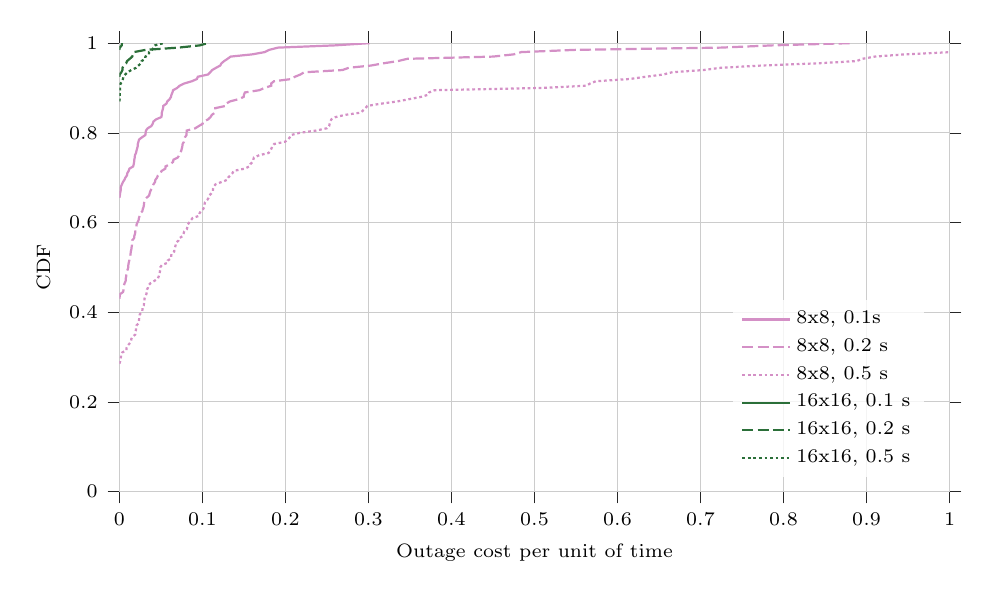
\begin{tikzpicture}

% \definecolor{color0}{rgb}{0.298039215686275,0.447058823529412,0.690196078431373}
% \definecolor{color1}{rgb}{0.866666666666667,0.517647058823529,0.32156862745098}

\definecolor{color0}{rgb}{0.17004232121058,0.436797596475173,0.223725555555555}
\definecolor{color1}{rgb}{0.82995767878942,0.563202403524827,0.776274444444444}

\begin{axis}[
axis line style={white!80!black},
legend cell align={left},
legend style={fill opacity=0.8, draw opacity=1, text opacity=1, at={(0.97,0.03)}, anchor=south east, draw=none},
tick align=outside,
tick pos=both,
% title={outage\_time offset 3dB, update period 0.1s, height 40m},
x grid style={white!80!black},
xlabel={Outage cost per unit of time},
xmajorgrids,
xmin=0, xmax=1,
xtick style={color=white!15!black},
y grid style={white!80!black},
ylabel={CDF},
ymajorgrids,
ymin=0, ymax=1,
ytick style={color=white!15!black}
]
\addplot [thick, color1]
table {%
0 0.655
0.00057142857142859 0.66
0.000872600349040157 0.665
0.00152827305145191 0.67
0.00163599182004096 0.675
0.00187149095446044 0.68
0.00309597523219812 0.685
0.0042839657282741 0.69
0.0060465116279072 0.695
0.00725255972696274 0.7
0.00917431192660545 0.705
0.00959947037404832 0.71
0.0112500000000003 0.715
0.012141280353201 0.72
0.0166032514700797 0.725
0.0173333333333333 0.73
0.0177838577291381 0.735
0.0179948586118256 0.74
0.0185325264750384 0.745
0.0187500000000001 0.75
0.0200668896321066 0.755
0.0206611570247929 0.76
0.0213887166769991 0.765
0.0221402214022139 0.77
0.0222297069720445 0.775
0.0229885057471263 0.78
0.0237399561723891 0.785
0.0273049645390075 0.79
0.0313325783314468 0.795
0.0317002881844378 0.8
0.0320197044334982 0.805
0.0340836012861746 0.81
0.038480513073509 0.815
0.0401721664275477 0.82
0.0410022779043295 0.825
0.0442511346444795 0.83
0.0505663430420732 0.835
0.0511221945137173 0.84
0.0511727078891264 0.845
0.0519125683060119 0.85
0.0526504297994279 0.855
0.0529435005926532 0.86
0.0566873339238275 0.865
0.0576923076923075 0.87
0.0605833956619312 0.875
0.0621370499419262 0.88
0.062764456981666 0.885
0.0639581657280798 0.89
0.0647118301314482 0.895
0.0696168375607147 0.9
0.0725156669650878 0.905
0.0781893004115236 0.91
0.0872954014029639 0.915
0.0934579439252356 0.92
0.0944851523332083 0.925
0.106701940035275 0.93
0.109467455621301 0.935
0.111801242236024 0.94
0.116497829232999 0.945
0.121468926553674 0.95
0.122994652406418 0.955
0.126213592233009 0.96
0.130303030303029 0.965
0.134011874469892 0.97
0.160250671441364 0.975
0.174999999999999 0.98
0.180451127819548 0.985
0.191158900836321 0.99
0.259437751004022 0.995
0.301458670988652 1
};
\addlegendentry{8x8, 0.1s}
\addplot [thick, color1, dash pattern=on 4pt off 1.5pt]
table {%
0 0.43
0.000397140587768086 0.435
0.000765403750478404 0.44
0.00452488687782805 0.445
0.00501367365542407 0.45
0.00514285714285731 0.455
0.00558139534883742 0.46
0.00644067796610173 0.465
0.00765794511806021 0.47
0.00767263427109969 0.475
0.00823045267489735 0.48
0.00843585237258359 0.485
0.00872219799389479 0.49
0.0100000000000003 0.495
0.0107612594659231 0.5
0.0107991360691144 0.505
0.0112676056338033 0.51
0.011945392491468 0.515
0.0125130344108448 0.52
0.0131578947368419 0.525
0.0138017565872021 0.535
0.0144369586140522 0.54
0.0147783251231526 0.545
0.0151898734177214 0.55
0.0152267461105594 0.555
0.0154405086285201 0.56
0.0177838577291381 0.565
0.0179968701095466 0.57
0.0189189189189188 0.575
0.0192307692307692 0.58
0.0193679918450563 0.585
0.020506634499397 0.59
0.0206718346253228 0.595
0.0217917675544796 0.6
0.0231404958677684 0.605
0.0235602094240842 0.61
0.0245839636913775 0.615
0.0250885478158199 0.62
0.0276679841897228 0.625
0.0282485875706223 0.63
0.0292184075967866 0.635
0.0296396092960594 0.64
0.0298965120735925 0.645
0.0306881587104769 0.65
0.0327198364008193 0.655
0.0358490566037733 0.66
0.036524822695036 0.665
0.0373333333333333 0.67
0.0387149917627692 0.675
0.0397350993377487 0.68
0.0410509031198695 0.685
0.042889390519187 0.69
0.0434126085315227 0.695
0.0453872718302927 0.7
0.0464396284829719 0.705
0.0495461422087762 0.71
0.0509325681492122 0.715
0.0554207119741122 0.72
0.055555555555555 0.725
0.061162079510703 0.73
0.0646630236794183 0.735
0.0651862464183393 0.74
0.0704488778054884 0.745
0.0720092915214846 0.75
0.0733485193621895 0.755
0.0745501285347062 0.76
0.0752212389380561 0.765
0.0758842443729926 0.77
0.076163610719325 0.775
0.0777860882572944 0.78
0.0781893004115224 0.785
0.0790201501382884 0.79
0.0808897876643102 0.795
0.0809498111171101 0.8
0.0811808118081177 0.805
0.0913160250671476 0.81
0.0956521739130432 0.815
0.100269957578099 0.82
0.100974313551818 0.825
0.106995884773664 0.83
0.109737248840803 0.835
0.111457521434141 0.84
0.115151515151514 0.845
0.115384615384615 0.85
0.115520282186951 0.855
0.128075253256154 0.86
0.128509045539617 0.865
0.133262260127933 0.87
0.143491124260354 0.875
0.149732620320857 0.88
0.150127226463107 0.885
0.151231945624472 0.89
0.168549905838044 0.895
0.174757281553397 0.9
0.182879377431906 0.905
0.182926829268291 0.91
0.18621307072516 0.915
0.207650273224042 0.92
0.21146953405018 0.925
0.218045112781953 0.93
0.222570532915359 0.935
0.268749999999998 0.94
0.27630522088354 0.945
0.303030303030302 0.95
0.318007662835248 0.955
0.335664335664337 0.96
0.346839546191245 0.965
0.450184501845017 0.97
0.475155279503103 0.975
0.484149855907778 0.98
0.549342105263155 0.985
0.724489795918367 0.99
0.786729857819904 0.995
0.881250000000002 1
};
\addlegendentry{8x8, 0.2 s}
\addplot [thick, color1, dash pattern=on 1pt off 1pt]
table {%
0 0.285
0.000936329588014997 0.29
0.00146627565982404 0.295
0.00191846522781782 0.3
0.00209095661265036 0.305
0.00349956255468073 0.31
0.00849473326537551 0.315
0.00859106529209639 0.32
0.00993377483443748 0.325
0.0122464600076545 0.33
0.0142630744849444 0.335
0.0144186046511633 0.34
0.0158604282315626 0.345
0.0191311279394189 0.35
0.019175846593228 0.355
0.0200000000000006 0.36
0.0201958384332932 0.365
0.0205198358413132 0.37
0.0230134607034312 0.375
0.0234641638225265 0.38
0.0238331678252234 0.385
0.0241796200345421 0.39
0.0245714285714294 0.395
0.0274576271186442 0.4
0.0277777777777775 0.405
0.0278174037089879 0.41
0.0294924554183822 0.415
0.029626253418415 0.42
0.0301810865191159 0.425
0.0302297460701339 0.43
0.0312699425654125 0.435
0.0324675324675336 0.44
0.0332065029401594 0.445
0.0332898172323769 0.45
0.0345336481700109 0.455
0.035149384885765 0.46
0.0378214826021192 0.465
0.0424528301886788 0.47
0.0463779225757011 0.475
0.0474799123447783 0.48
0.0482109227871955 0.485
0.0488443087658108 0.49
0.0490093847758087 0.495
0.0492870427774326 0.5
0.0512311358220831 0.505
0.0579029733959325 0.51
0.0582687773661167 0.515
0.062160828811053 0.52
0.062423500611994 0.525
0.0627836611195179 0.53
0.0660377358490567 0.535
0.0663430420712 0.54
0.0671902268760921 0.545
0.0678241996744461 0.55
0.0683254344391812 0.555
0.0715181932245924 0.56
0.0724533715925414 0.565
0.0763546798029573 0.57
0.0773333333333333 0.575
0.0781108083560429 0.58
0.0812499999999992 0.585
0.0819604612850115 0.59
0.0822085889570584 0.595
0.084220127698387 0.6
0.0860927152317889 0.605
0.0883424408014588 0.61
0.096246390760348 0.615
0.0965018094089269 0.62
0.0979498861047872 0.625
0.101002865329515 0.63
0.10246052148366 0.635
0.102574416733713 0.64
0.103077816492448 0.645
0.105774419859691 0.65
0.10762331838565 0.655
0.108257605689455 0.66
0.110972568578557 0.665
0.112610875433865 0.67
0.112834978843444 0.675
0.113687359760661 0.68
0.11575562700965 0.685
0.122649955237247 0.69
0.129860324650816 0.695
0.130925507900676 0.7
0.133687943262413 0.705
0.136222910216717 0.71
0.13756613756614 0.715
0.15086646279307 0.72
0.156581409856524 0.725
0.15766738660907 0.73
0.160606060606059 0.735
0.161360347322725 0.74
0.162079510703363 0.745
0.168521462639108 0.75
0.17980513728964 0.755
0.18181818181818 0.76
0.183206106870233 0.765
0.18421052631579 0.77
0.186355022109923 0.775
0.199488491048592 0.78
0.203235591506579 0.785
0.20534759358289 0.79
0.206642066420663 0.795
0.217455621301774 0.8
0.236947791164664 0.805
0.249701314217445 0.81
0.252688172043011 0.815
0.253312548713958 0.82
0.254237288135597 0.825
0.255319148936171 0.83
0.260288065843625 0.835
0.271844660194173 0.84
0.290726817042604 0.845
0.293643688451214 0.85
0.296516567544611 0.855
0.298642533936651 0.86
0.315270935960589 0.865
0.334928229665071 0.87
0.349056603773582 0.875
0.363214837712516 0.88
0.372093023255811 0.885
0.373134328358213 0.89
0.379746835443035 0.895
0.507692307692306 0.9
0.562499999999995 0.905
0.567099567099566 0.91
0.573913043478259 0.915
0.614634146341459 0.92
0.633879781420761 0.925
0.6551724137931 0.93
0.665706051873195 0.935
0.703403565640188 0.940000000000001
0.724279835390944 0.945000000000001
0.77302631578947 0.950000000000001
0.841328413284129 0.955000000000001
0.88811188811189 0.960000000000001
0.894941634241242 0.965000000000001
0.909937888198752 0.970000000000001
0.946360153256701 0.975000000000001
1.0027027027027 0.980000000000001
1.00473933649289 0.985000000000001
1.00510204081633 0.990000000000001
1.00625 0.995000000000001
1.00709219858156 1
};
\addlegendentry{8x8, 0.5 s}
\addplot [thick, color0]
table {%
0 0.985
0.000455580865603662 0.99
0.00288184438040344 0.995
0.00310559006211178 1
};
\addlegendentry{16x16, 0.1 s}
\addplot [thick, color0, dash pattern=on 4pt off 1.5pt]
table {%
0 0.925
0.000455580865603662 0.93
0.00243902439024388 0.935
0.00369003690036899 0.94
0.00383141762452106 0.945
0.0052730696798495 0.95
0.00819672131147535 0.955
0.00927357032457488 0.96
0.012539184952978 0.965
0.0155279503105589 0.97
0.0164473684210525 0.975
0.0173160173160173 0.98
0.0317002881844378 0.985
0.0710900473933648 0.99
0.0969387755102041 0.995
0.10625 1
};
\addlegendentry{16x16, 0.2 s}
\addplot [thick, color0, dash pattern=on 1pt off 1pt]
table {%
0 0.87
0.000367242012486237 0.875
0.000377500943752371 0.88
0.000383288616328109 0.885
0.000402414486921545 0.89
0.000779423226812177 0.895
0.000885739592559804 0.9
0.000895255147717116 0.905
0.00152998776009789 0.91
0.00369003690036899 0.915
0.00434782608695651 0.92
0.00473933649289099 0.925
0.00699300699300701 0.93
0.00975609756097554 0.935
0.0144092219020172 0.94
0.0200927357032456 0.945
0.0230263157894736 0.95
0.0259740259740259 0.955
0.0268199233716474 0.96
0.0310559006211178 0.965
0.031347962382445 0.97
0.0355191256830599 0.975
0.0357142857142857 0.98
0.0394088669950736 0.985
0.0411522633744855 0.99
0.0428015564202333 0.995
0.0531645569620249 1
};
\addlegendentry{16x16, 0.5 s}
\end{axis}

\end{tikzpicture}

\caption{Outage cost for antenna array sizes of 64 and 256 antenna elements for different beam alignment intervals for a UAV flying at $40$~m above ground level.}
\label{fig:outage}
\end{figure}
\par Figure \ref{fig:handovers40} shows the number of handovers per minute for different antenna configurations of both a (a) 64-element and a (b) 256-element antenna array respectively at an altitude of $40$~m. The dashed line represents the baseline static scenario. A UAV in this scenario is mainly served by sidelobes resulting in larger numbers of handovers when compared to a beamsteering scenario. Additionally, increasing the number of antenna elements creates more sidelobes resulting in even worse handover rates as seen in \ref{fig:handovers40} (b). When considering beamsteering, for both numbers of antenna elements, the horizontal linear antenna array of 1 by 64 or 1 by 256 performs the worst of the set. This can be explained by the fact that from a BS perspective the relative movement of a UAV will mainly happen in the horizontal direction and a horizontal linear array generates narrow vertical plane shaped beam as shown in Figure \ref{fig:diff_top}. This shape results in the BS easily losing track of the user if it moves in the horizontal plane. The opposite is also true, a vertical linear array of 256 by 1 manages to track users moving in the horizontal plane, but lacks in its capabilities to track a user move towards/away from the BS. The square planar array should perform better in both planes perfectly, however users move in general more the horizontal plane. We could assume that a rectangular with slightly more antennas on the vertical axis should perform even better. Figure \ref{fig:handovers40} shows exactly this, an array of 16 by 4 or 64 by 4 elements slightly outperforms a default square array of the same number of antennas. We can also see that for larger antenna arrays the topology has more impact on the performance when compared to the results of the smaller antenna array.

\begin{figure}[t]
% \centerline{
% \includegraphics{handover_per_min}
% }
\centering
\begin{subfigure}[t]{\linewidth}
\caption{64-element antenna array}
% This file was created by tikzplotlib v0.9.3.
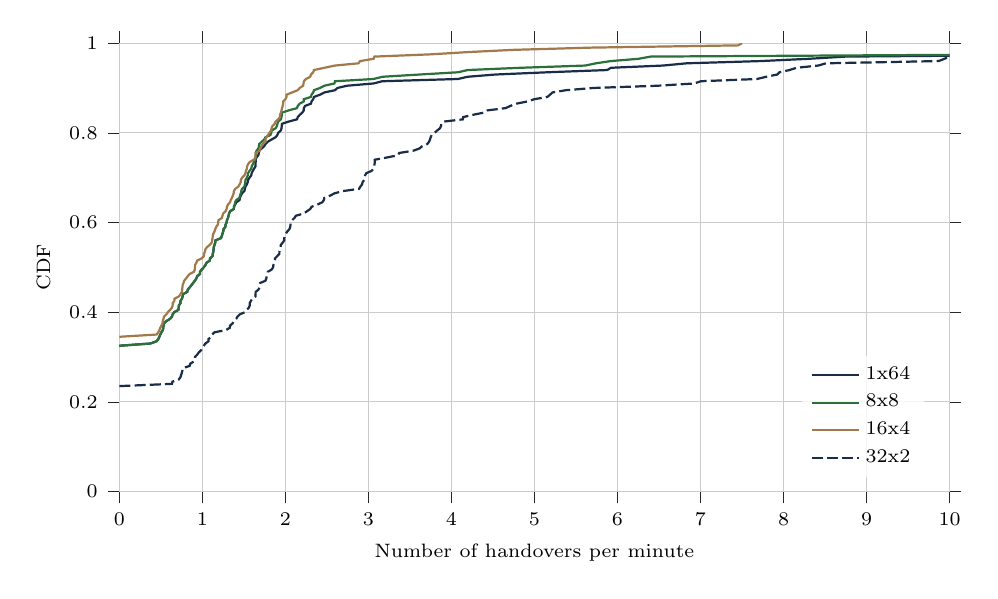
\begin{tikzpicture}

\definecolor{color0}{rgb}{0.0964154061637055,0.177286718595531,0.283473631853997}
\definecolor{color1}{rgb}{0.17004232121058,0.436797596475173,0.223725555555555}
\definecolor{color2}{rgb}{0.632842247501842,0.474798109622068,0.290702092080255}
\definecolor{color3}{rgb}{0.82995767878942,0.563202403524827,0.776274444444444}
\definecolor{color4}{rgb}{0.763267446283815,0.850242277575182,0.951553976205169}

\begin{axis}[
axis line style={white!80!black},
legend cell align={left},
legend style={fill opacity=0.8, draw opacity=1, text opacity=1, at={(0.97,0.03)}, anchor=south east, draw=none},
tick align=outside,
tick pos=both,
% title={h/t 40offset 3dB, update period 0.1s, height 40m},
x grid style={white!80!black},
xlabel={Number of handovers per minute},
xmajorgrids,
xmin=0, xmax=10,
xtick style={color=white!15!black},
y grid style={white!80!black},
ylabel={CDF},
ymajorgrids,
ymin=0, ymax=1,
ytick style={color=white!15!black}
]
\addplot [thick, color0]
table {%
0 0.325
0.374064837905248 0.33
0.448765893792083 0.335
0.469483568075128 0.34
0.481927710843384 0.345
0.492610837438434 0.35
0.505902192242843 0.355
0.523560209424094 0.36
0.529100529100539 0.365
0.531443755535883 0.37
0.53715308863027 0.375
0.564971751412439 0.38
0.611620795107042 0.385
0.632911392405071 0.39
0.641711229946531 0.395
0.662251655629145 0.4
0.710900473933678 0.405
0.714853057982554 0.41
0.716845878136205 0.415
0.736196319018408 0.42
0.736196319018434 0.425
0.752823086574657 0.43
0.762388818297334 0.435
0.765794511806021 0.44
0.817438692098123 0.445
0.823045267489735 0.45
0.846262341325834 0.455
0.868306801736636 0.46
0.8880118401579 0.465
0.909090909090902 0.47
0.927357032457487 0.475
0.937500000000022 0.48
0.970873786407805 0.485
0.971397733405321 0.49
0.991735537190073 0.495
1.01781170483463 0.5
1.0362694300518 0.505
1.04986876640422 0.51
1.08827085852482 0.515
1.09289617486341 0.52
1.12289457267627 0.525
1.12500000000003 0.53
1.1320754716981 0.535
1.13464447806358 0.54
1.13708149084021 0.545
1.14591291061883 0.55
1.15495668912418 0.555
1.15696104897806 0.56
1.22399020807838 0.565
1.23456790123458 0.57
1.24172185430468 0.575
1.25130344108448 0.58
1.25457396759022 0.585
1.27659574468087 0.59
1.27931769722816 0.595
1.29124820659975 0.6
1.29589632829373 0.605
1.30832969908422 0.61
1.3148283418554 0.615
1.32207124495045 0.62
1.33333333333332 0.625
1.37931034482758 0.63
1.37983901878119 0.635
1.39534883720935 0.64
1.40845070422538 0.645
1.4475271411339 0.65
1.45278450363198 0.655
1.46341463414633 0.66
1.47783251231526 0.665
1.50564617314931 0.67
1.51196976060485 0.675
1.51898734177214 0.68
1.53583617747446 0.685
1.54639175257735 0.69
1.55038759689921 0.695
1.56794425087104 0.7
1.58850226928901 0.705
1.59386068476974 0.71
1.60734787600465 0.715
1.62162162162161 0.72
1.63934426229507 0.725
1.64083865086606 0.73
1.64158686730506 0.735
1.64183642444509 0.74
1.65238678090572 0.745
1.67389956602601 0.75
1.68067226890758 0.755
1.68539325842699 0.76
1.71428571428577 0.765
1.74418604651162 0.77
1.75953079178885 0.775
1.78748758689176 0.78
1.8339276617423 0.785
1.8808777429467 0.79
1.90325138778751 0.795
1.91311279394189 0.8
1.94489465153969 0.805
1.95333695062405 0.81
1.95599022004894 0.815
1.958224543081 0.82
2.03873598369012 0.825
2.13980028530676 0.83
2.14899713467053 0.835
2.17216411906686 0.84
2.20318237454107 0.845
2.2222222222222 0.85
2.22222222222228 0.855
2.23728813559323 0.86
2.3076923076923 0.865
2.31511254019299 0.87
2.33463035019454 0.875
2.34476769431186 0.88
2.41718889883626 0.885
2.46913580246913 0.89
2.59740259740259 0.895
2.62714718760526 0.9
2.74165202108967 0.905
3.06122448979592 0.91
3.1654676258994 0.915
4.07816482582846 0.92
4.19580419580421 0.925
4.53001132502845 0.93
5.15672396359978 0.935
5.87570621468944 0.940000000000001
5.92105263157892 0.945000000000001
6.54715510522229 0.950000000000001
6.83371298405492 0.955000000000001
7.72635814889367 0.960000000000001
8.29711576452028 0.965000000000001
8.74999999999993 0.970000000000001
12.1037463976944 0.975000000000001
15.4981549815497 0.980000000000001
16.0919540229884 0.985000000000001
40.9937888198755 0.990000000000001
68.2464454976302 0.995000000000001
82.5000000000002 1
};
\addlegendentry{1x64}
\addplot [thick, color1]
table {%
0 0.325
0.374064837905248 0.33
0.448765893792083 0.335
0.469483568075128 0.34
0.481927710843384 0.345
0.492610837438434 0.35
0.505902192242843 0.355
0.523560209424094 0.36
0.529100529100539 0.365
0.531443755535883 0.37
0.53715308863027 0.375
0.564971751412439 0.38
0.611620795107042 0.385
0.632911392405071 0.39
0.641711229946531 0.395
0.662251655629145 0.4
0.710900473933678 0.405
0.714853057982554 0.41
0.716845878136205 0.415
0.736196319018408 0.42
0.736196319018434 0.425
0.752823086574657 0.43
0.762388818297334 0.435
0.765794511806021 0.44
0.817438692098123 0.445
0.823045267489735 0.45
0.846262341325834 0.455
0.868306801736636 0.46
0.8880118401579 0.465
0.909090909090902 0.47
0.927357032457487 0.475
0.937500000000022 0.48
0.970873786407805 0.485
0.971397733405321 0.49
0.991735537190073 0.495
1.01781170483463 0.5
1.0362694300518 0.505
1.04986876640422 0.51
1.08827085852482 0.515
1.09289617486341 0.52
1.12289457267627 0.525
1.12500000000003 0.53
1.1320754716981 0.535
1.13464447806358 0.54
1.13708149084021 0.545
1.14591291061883 0.55
1.15495668912418 0.555
1.15696104897806 0.56
1.22399020807838 0.565
1.23456790123458 0.57
1.24172185430468 0.575
1.25130344108448 0.58
1.25457396759022 0.585
1.27659574468087 0.59
1.27931769722816 0.595
1.29124820659975 0.6
1.29589632829373 0.605
1.30832969908422 0.61
1.3148283418554 0.615
1.32207124495045 0.62
1.33333333333332 0.625
1.37931034482758 0.63
1.37983901878119 0.635
1.39026812313803 0.64
1.39534883720935 0.645
1.40845070422538 0.65
1.4475271411339 0.655
1.45278450363198 0.66
1.46341463414633 0.665
1.46878824969405 0.67
1.47783251231526 0.675
1.50564617314931 0.68
1.51196976060485 0.685
1.51668351870582 0.69
1.51898734177214 0.695
1.53583617747446 0.7
1.54639175257735 0.705
1.55038759689921 0.71
1.56794425087104 0.715
1.58850226928901 0.72
1.59386068476974 0.725
1.60734787600465 0.73
1.62162162162161 0.735
1.63934426229507 0.74
1.64083865086606 0.745
1.64158686730506 0.75
1.64183642444509 0.755
1.65238678090572 0.76
1.67389956602601 0.765
1.68067226890758 0.77
1.68539325842699 0.775
1.71428571428577 0.78
1.74418604651162 0.785
1.75953079178885 0.79
1.81879420680364 0.795
1.83050847457628 0.8
1.8339276617423 0.805
1.8808777429467 0.81
1.89806678383131 0.815
1.90325138778751 0.82
1.91311279394189 0.825
1.94489465153969 0.83
1.95333695062405 0.835
1.95599022004894 0.84
1.958224543081 0.845
2.03873598369012 0.85
2.13980028530676 0.855
2.14899713467053 0.86
2.17216411906686 0.865
2.2222222222222 0.87
2.22222222222228 0.875
2.3076923076923 0.88
2.31511254019299 0.885
2.33463035019454 0.89
2.34476769431186 0.895
2.41718889883626 0.9
2.46913580246913 0.905
2.58992805755405 0.91
2.59740259740259 0.915
3.06122448979592 0.92
3.17100792751992 0.925
3.61581920903966 0.93
4.07816482582846 0.935
4.19580419580421 0.940000000000001
4.82897384305854 0.945000000000001
5.61184723304768 0.950000000000001
5.74031890660614 0.955000000000001
5.92105263157892 0.960000000000001
6.24999999999995 0.965000000000001
6.40063216120136 0.970000000000001
11.070110701107 0.975000000000001
12.1037463976944 0.980000000000001
16.0919540229884 0.985000000000001
40.9937888198755 0.990000000000001
51.1848341232227 0.995000000000001
67.5000000000002 1
};
\addlegendentry{8x8}
\addplot [thick, color2]
table {%
0 0.345
0.448765893792083 0.35
0.469483568075128 0.355
0.481927710843384 0.36
0.492610837438434 0.365
0.505902192242843 0.37
0.519930675909889 0.375
0.523560209424094 0.38
0.531443755535883 0.385
0.53715308863027 0.39
0.564971751412439 0.395
0.584795321637436 0.4
0.611620795107042 0.405
0.632911392405071 0.41
0.641711229946531 0.415
0.642398286937909 0.42
0.662251655629145 0.425
0.66481994459836 0.43
0.716845878136205 0.435
0.736196319018408 0.44
0.752823086574657 0.445
0.756620428751599 0.45
0.759493670886078 0.455
0.762388818297334 0.46
0.771704180064331 0.465
0.781250000000001 0.47
0.802139037433178 0.475
0.823045267489735 0.48
0.846262341325834 0.485
0.897531787584166 0.49
0.909090909090902 0.495
0.909780136467043 0.5
0.910931174089101 0.505
0.927357032457487 0.51
0.937500000000022 0.515
0.991735537190073 0.52
1.01781170483463 0.525
1.01954120645712 0.53
1.03092783505157 0.535
1.0362694300518 0.54
1.05633802816903 0.545
1.08827085852482 0.55
1.113172541744 0.555
1.11731843575423 0.56
1.12289457267627 0.565
1.12429731417867 0.57
1.1320754716981 0.575
1.14591291061883 0.58
1.15495668912418 0.585
1.16580310880832 0.59
1.18530225207433 0.595
1.19165839126117 0.6
1.19284294234597 0.605
1.23456790123458 0.61
1.24172185430468 0.615
1.24999999999999 0.62
1.27931769722816 0.625
1.29124820659975 0.63
1.29589632829373 0.635
1.30832969908422 0.64
1.33333333333332 0.645
1.34128166915055 0.65
1.35669869983046 0.655
1.36674259681098 0.66
1.37614678899084 0.665
1.37931034482758 0.67
1.39534883720935 0.675
1.43312101910831 0.68
1.44810941271124 0.685
1.46163215590749 0.69
1.46341463414633 0.695
1.47783251231526 0.7
1.50564617314931 0.705
1.51898734177214 0.71
1.52413209144796 0.715
1.53583617747446 0.72
1.53846153846154 0.725
1.55038759689921 0.73
1.57068062827225 0.735
1.62162162162161 0.74
1.63934426229507 0.745
1.64083865086606 0.75
1.64158686730506 0.755
1.68855534709196 0.76
1.69971671388101 0.765
1.7094017094017 0.77
1.72910662824206 0.775
1.75953079178885 0.78
1.75953079178891 0.785
1.76991150442481 0.79
1.79015415216317 0.795
1.80722891566264 0.8
1.82717929196809 0.805
1.83299389002038 0.81
1.84426229508199 0.815
1.87061574434923 0.82
1.8808777429467 0.825
1.91311279394189 0.83
1.93409742120347 0.835
1.93548387096779 0.84
1.94489465153969 0.845
1.95333695062405 0.85
1.96721311475408 0.86
1.97260273972609 0.865
1.97368421052631 0.87
1.99999999999998 0.875
2.01342281879196 0.88
2.01438848920871 0.885
2.07972270363949 0.89
2.14861235452112 0.895
2.17216411906686 0.9
2.21402214022139 0.905
2.21811460258778 0.91
2.2222222222222 0.915
2.24719101123593 0.92
2.29885057471263 0.925
2.3076923076923 0.93
2.33463035019454 0.935
2.34476769431186 0.940000000000001
2.46913580246913 0.945000000000001
2.59740259740259 0.950000000000001
2.87999999999997 0.955000000000001
2.9001074113857 0.960000000000001
3.06122448979592 0.965000000000001
3.0729833546735 0.970000000000001
3.75000000000001 0.975000000000001
4.19580419580421 0.980000000000001
4.74683544303793 0.985000000000001
5.68720379146919 0.990000000000001
7.45341614906828 0.995000000000001
7.50000000000002 1
};
\addlegendentry{16x4}
% \addplot [thick, color3]
% table {%
% 0 0.325
% 0.374064837905248 0.33
% 0.448765893792083 0.335
% 0.469483568075128 0.34
% 0.481927710843384 0.345
% 0.492610837438434 0.35
% 0.505902192242843 0.355
% 0.523560209424094 0.36
% 0.529100529100539 0.365
% 0.531443755535883 0.37
% 0.53715308863027 0.375
% 0.564971751412439 0.38
% 0.611620795107042 0.385
% 0.632911392405071 0.39
% 0.641711229946531 0.395
% 0.662251655629145 0.4
% 0.710900473933678 0.405
% 0.714853057982554 0.41
% 0.716845878136205 0.415
% 0.736196319018408 0.42
% 0.736196319018434 0.425
% 0.752823086574657 0.43
% 0.762388818297334 0.435
% 0.765794511806021 0.44
% 0.817438692098123 0.445
% 0.823045267489735 0.45
% 0.846262341325834 0.455
% 0.868306801736636 0.46
% 0.8880118401579 0.465
% 0.909090909090902 0.47
% 0.927357032457487 0.475
% 0.937500000000022 0.48
% 0.970873786407805 0.485
% 0.971397733405321 0.49
% 0.991735537190073 0.495
% 1.01781170483463 0.5
% 1.0362694300518 0.505
% 1.04986876640422 0.51
% 1.08827085852482 0.515
% 1.09289617486341 0.52
% 1.12289457267627 0.525
% 1.12500000000003 0.53
% 1.1320754716981 0.535
% 1.13464447806358 0.54
% 1.13708149084021 0.545
% 1.14591291061883 0.55
% 1.15495668912418 0.555
% 1.15696104897806 0.56
% 1.22399020807838 0.565
% 1.23456790123458 0.57
% 1.24172185430468 0.575
% 1.25130344108448 0.58
% 1.25457396759022 0.585
% 1.27659574468087 0.59
% 1.27931769722816 0.595
% 1.29124820659975 0.6
% 1.29589632829373 0.605
% 1.30832969908422 0.61
% 1.3148283418554 0.615
% 1.32207124495045 0.62
% 1.33333333333332 0.625
% 1.37931034482758 0.63
% 1.37983901878119 0.635
% 1.39026812313803 0.64
% 1.39534883720935 0.645
% 1.40845070422538 0.65
% 1.4475271411339 0.655
% 1.45278450363198 0.66
% 1.46341463414633 0.665
% 1.46878824969405 0.67
% 1.47783251231526 0.675
% 1.50564617314931 0.68
% 1.51196976060485 0.685
% 1.51668351870582 0.69
% 1.51898734177214 0.695
% 1.53583617747446 0.7
% 1.54639175257735 0.705
% 1.55038759689921 0.71
% 1.56794425087104 0.715
% 1.58850226928901 0.72
% 1.59386068476974 0.725
% 1.60734787600465 0.73
% 1.62162162162161 0.735
% 1.63934426229507 0.74
% 1.64083865086606 0.745
% 1.64158686730506 0.75
% 1.64183642444509 0.755
% 1.65238678090572 0.76
% 1.67389956602601 0.765
% 1.68067226890758 0.77
% 1.68539325842699 0.775
% 1.71428571428577 0.78
% 1.74418604651162 0.785
% 1.75953079178885 0.79
% 1.81879420680364 0.795
% 1.83050847457628 0.8
% 1.8339276617423 0.805
% 1.8808777429467 0.81
% 1.89806678383131 0.815
% 1.90325138778751 0.82
% 1.91311279394189 0.825
% 1.94489465153969 0.83
% 1.95333695062405 0.835
% 1.95599022004894 0.84
% 1.958224543081 0.845
% 2.03873598369012 0.85
% 2.13980028530676 0.855
% 2.14899713467053 0.86
% 2.17216411906686 0.865
% 2.2222222222222 0.87
% 2.22222222222228 0.875
% 2.3076923076923 0.88
% 2.31511254019299 0.885
% 2.33463035019454 0.89
% 2.34476769431186 0.895
% 2.41718889883626 0.9
% 2.46913580246913 0.905
% 2.58992805755405 0.91
% 2.59740259740259 0.915
% 3.06122448979592 0.92
% 3.17100792751992 0.925
% 3.61581920903966 0.93
% 4.07816482582846 0.935
% 4.19580419580421 0.940000000000001
% 4.82897384305854 0.945000000000001
% 5.61184723304768 0.950000000000001
% 5.74031890660614 0.955000000000001
% 5.92105263157892 0.960000000000001
% 6.24999999999995 0.965000000000001
% 6.40063216120136 0.970000000000001
% 11.070110701107 0.975000000000001
% 12.1037463976944 0.980000000000001
% 16.0919540229884 0.985000000000001
% 40.9937888198755 0.990000000000001
% 51.1848341232227 0.995000000000001
% 67.5000000000002 1
% };
% \addlegendentry{32x2}
% \addplot [thick, color4]
% table {%
% 0 0.325
% 0.374064837905248 0.33
% 0.448765893792083 0.335
% 0.469483568075128 0.34
% 0.481927710843384 0.345
% 0.492610837438434 0.35
% 0.505902192242843 0.355
% 0.523560209424094 0.36
% 0.529100529100539 0.365
% 0.531443755535883 0.37
% 0.53715308863027 0.375
% 0.564971751412439 0.38
% 0.611620795107042 0.385
% 0.632911392405071 0.39
% 0.641711229946531 0.395
% 0.662251655629145 0.4
% 0.710900473933678 0.405
% 0.714853057982554 0.41
% 0.716845878136205 0.415
% 0.736196319018408 0.42
% 0.736196319018434 0.425
% 0.752823086574657 0.43
% 0.762388818297334 0.435
% 0.765794511806021 0.44
% 0.817438692098123 0.445
% 0.823045267489735 0.45
% 0.846262341325834 0.455
% 0.868306801736636 0.46
% 0.8880118401579 0.465
% 0.909090909090902 0.47
% 0.927357032457487 0.475
% 0.937500000000022 0.48
% 0.970873786407805 0.485
% 0.971397733405321 0.49
% 0.991735537190073 0.495
% 1.01781170483463 0.5
% 1.0362694300518 0.505
% 1.04986876640422 0.51
% 1.08827085852482 0.515
% 1.09289617486341 0.52
% 1.12289457267627 0.525
% 1.12500000000003 0.53
% 1.1320754716981 0.535
% 1.13464447806358 0.54
% 1.13708149084021 0.545
% 1.14591291061883 0.55
% 1.15495668912418 0.555
% 1.15696104897806 0.56
% 1.22399020807838 0.565
% 1.23456790123458 0.57
% 1.24172185430468 0.575
% 1.25130344108448 0.58
% 1.25457396759022 0.585
% 1.27659574468087 0.59
% 1.27931769722816 0.595
% 1.29124820659975 0.6
% 1.29589632829373 0.605
% 1.30832969908422 0.61
% 1.3148283418554 0.615
% 1.32207124495045 0.62
% 1.33333333333332 0.625
% 1.37931034482758 0.63
% 1.37983901878119 0.635
% 1.39026812313803 0.64
% 1.39534883720935 0.645
% 1.40845070422538 0.65
% 1.4475271411339 0.655
% 1.45278450363198 0.66
% 1.46341463414633 0.665
% 1.46878824969405 0.67
% 1.47783251231526 0.675
% 1.50564617314931 0.68
% 1.51196976060485 0.685
% 1.51668351870582 0.69
% 1.51898734177214 0.695
% 1.53583617747446 0.7
% 1.54639175257735 0.705
% 1.55038759689921 0.71
% 1.56794425087104 0.715
% 1.58850226928901 0.72
% 1.59386068476974 0.725
% 1.60734787600465 0.73
% 1.62162162162161 0.735
% 1.63934426229507 0.74
% 1.64083865086606 0.745
% 1.64158686730506 0.75
% 1.64183642444509 0.755
% 1.65238678090572 0.76
% 1.67389956602601 0.765
% 1.68067226890758 0.77
% 1.68539325842699 0.775
% 1.71428571428577 0.78
% 1.74418604651162 0.785
% 1.75953079178885 0.79
% 1.81879420680364 0.795
% 1.83050847457628 0.8
% 1.8339276617423 0.805
% 1.8808777429467 0.81
% 1.89806678383131 0.815
% 1.90325138778751 0.82
% 1.91311279394189 0.825
% 1.94489465153969 0.83
% 1.95333695062405 0.835
% 1.95599022004894 0.84
% 1.958224543081 0.845
% 2.03873598369012 0.85
% 2.13980028530676 0.855
% 2.14899713467053 0.86
% 2.17216411906686 0.865
% 2.2222222222222 0.87
% 2.22222222222228 0.875
% 2.3076923076923 0.88
% 2.31511254019299 0.885
% 2.33463035019454 0.89
% 2.34476769431186 0.895
% 2.41718889883626 0.9
% 2.46913580246913 0.905
% 2.58992805755405 0.91
% 2.59740259740259 0.915
% 3.06122448979592 0.92
% 3.17100792751992 0.925
% 4.06779661016962 0.93
% 4.07816482582846 0.935
% 4.19580419580421 0.940000000000001
% 5.3118712273644 0.945000000000001
% 5.61184723304768 0.950000000000001
% 5.92105263157892 0.955000000000001
% 6.24999999999995 0.960000000000001
% 6.28701594533053 0.965000000000001
% 6.87475306203109 0.970000000000001
% 11.070110701107 0.975000000000001
% 12.1037463976944 0.980000000000001
% 16.0919540229884 0.985000000000001
% 40.9937888198755 0.990000000000001
% 56.8720379146919 0.995000000000001
% 82.5000000000002 1
% };
% \addlegendentry{64x1}
\addplot [thick, color0, dash pattern=on 4pt off 1.5pt]
table {%
0 0.235
0.632911392405071 0.24
0.63965884861408 0.245
0.716845878136205 0.25
0.736196319018408 0.255
0.752823086574657 0.265
0.759493670886078 0.27
0.762388818297334 0.275
0.846262341325834 0.28
0.854700854700851 0.285
0.897531787584166 0.29
0.909090909090902 0.295
0.910931174089101 0.3
0.937500000000022 0.305
0.955414012738875 0.31
0.985221674876869 0.315
0.993377483443747 0.32
1.01781170483463 0.325
1.0362694300518 0.33
1.07334525939176 0.335
1.07430617726054 0.34
1.10905730129389 0.345
1.11731843575423 0.35
1.14591291061883 0.355
1.28342245989306 0.36
1.32963988919672 0.365
1.33333333333332 0.37
1.36467020470056 0.375
1.37931034482758 0.38
1.40845070422538 0.385
1.42236270248919 0.39
1.45102781136643 0.395
1.5132408575032 0.4
1.53583617747446 0.405
1.55979202772967 0.41
1.57068062827225 0.415
1.57068062827228 0.42
1.58450704225355 0.425
1.6 0.43
1.63934426229507 0.435
1.64083865086606 0.44
1.64158686730506 0.445
1.67441860465122 0.45
1.68855534709196 0.455
1.68946098149645 0.46
1.69491525423728 0.465
1.75953079178885 0.47
1.76991150442481 0.475
1.77514792899407 0.48
1.78571428571427 0.485
1.78837555886741 0.49
1.83486238532113 0.495
1.85185185185188 0.5
1.85528756957334 0.505
1.87149095446044 0.51
1.87382885696445 0.515
1.87499999999998 0.52
1.90174326465925 0.525
1.92719486081373 0.53
1.92771084337354 0.535
1.93548387096773 0.54
1.94300518134721 0.545
1.94489465153969 0.55
1.96721311475408 0.555
1.98609731876862 0.56
1.98675496688744 0.565
1.99004975124376 0.57
2.00534759358294 0.575
2.02360876897137 0.58
2.04778156996586 0.585
2.05761316872434 0.59
2.06185567010313 0.595
2.06422018348625 0.6
2.07972270363949 0.605
2.10896309314585 0.61
2.12577502214353 0.615
2.2222222222222 0.62
2.25988700564975 0.625
2.29885057471263 0.63
2.31511254019299 0.635
2.38568588469193 0.64
2.4439918533605 0.645
2.46334310850448 0.65
2.46913580246913 0.655
2.54022015241326 0.66
2.59179265658745 0.665
2.6925953627525 0.67
2.88739172281044 0.675
2.90322580645168 0.68
2.92397660818718 0.685
2.93000542593607 0.69
2.95081967213112 0.695
2.95566502463055 0.7
2.95890410958914 0.705
2.97520661157022 0.71
3.03797468354428 0.715
3.06122448979592 0.72
3.06905370843988 0.725
3.07377049180332 0.73
3.07692307692308 0.735
3.07692307692308 0.74
3.2258064516129 0.745
3.35570469798661 0.75
3.3707865168539 0.755
3.53982300884954 0.76
3.61445783132528 0.765
3.647416413374 0.77
3.70942812982995 0.775
3.73092142453376 0.78
3.74100719424474 0.785
3.75000000000001 0.79
3.76175548589339 0.795
3.79746835443034 0.8
3.82687927107076 0.805
3.86162510056331 0.81
3.87374461979924 0.815000000000001
3.87866732968686 0.820000000000001
3.90625 0.825000000000001
4.13793103448277 0.830000000000001
4.14129110840455 0.835000000000001
4.25531914893618 0.840000000000001
4.39024390243899 0.845000000000001
4.43349753694578 0.850000000000001
4.65116279069764 0.855000000000001
4.70998691670319 0.860000000000001
4.78278198485471 0.865000000000001
4.91803278688523 0.870000000000001
4.99999999999996 0.875000000000001
5.15574650913014 0.880000000000001
5.18731988472619 0.885000000000001
5.21739130434781 0.890000000000001
5.37772087067863 0.895000000000001
5.70993528740027 0.900000000000001
6.48648648648644 0.905000000000001
6.9230769230769 0.910000000000001
7.00389105058363 0.915000000000001
7.67999999999992 0.920000000000001
7.79220779220777 0.925000000000001
7.92452830188672 0.930000000000001
7.95128939828094 0.935000000000001
8.07174887892375 0.940000000000001
8.15632965165692 0.945000000000001
8.41777084957151 0.950000000000001
8.51063829787236 0.955000000000001
9.86842105263153 0.960000000000001
9.93733213966018 0.965000000000001
9.9999999999999 0.970000000000001
11.25 0.975000000000001
11.3744075829384 0.980000000000001
14.9068322981366 0.985000000000001
17.7121771217711 0.990000000000001
20.979020979021 0.995000000000001
41.3793103448276 1
};
\addlegendentry{32x2}
% \addplot [semithick, color0, dash pattern=on 4pt off 1.5pt]
% table {%
% 0 0.3
% 0.469483568075128 0.305
% 0.505902192242843 0.31
% 0.523560209424094 0.315
% 0.611620795107042 0.32
% 0.632911392405071 0.325
% 0.642398286937909 0.33
% 0.662251655629145 0.335
% 0.716845878136205 0.34
% 0.736196319018408 0.345
% 0.752823086574657 0.355
% 0.759493670886078 0.36
% 0.762388818297334 0.365
% 0.781250000000001 0.37
% 0.894632206759475 0.375
% 0.897531787584166 0.38
% 0.909090909090902 0.385
% 0.909780136467043 0.39
% 0.910931174089101 0.395
% 0.927357032457487 0.4
% 0.937500000000022 0.405
% 0.955414012738875 0.41
% 0.985221674876869 0.415
% 0.991735537190073 0.42
% 0.993377483443747 0.425
% 0.99722991689754 0.43
% 1.01781170483463 0.435
% 1.0362694300518 0.44
% 1.03986135181978 0.445
% 1.06288751107177 0.45
% 1.10905730129389 0.455
% 1.11731843575423 0.46
% 1.12570356472797 0.465
% 1.12994350282488 0.47
% 1.1349306431274 0.475
% 1.14591291061883 0.48
% 1.15495668912418 0.485
% 1.16580310880832 0.49
% 1.16959064327487 0.495
% 1.20675784392603 0.5
% 1.26939351198875 0.505
% 1.27931769722816 0.51
% 1.28342245989306 0.515
% 1.29589632829373 0.52
% 1.33333333333332 0.525
% 1.34629768137625 0.53
% 1.36736554238838 0.535
% 1.37931034482758 0.54
% 1.42236270248919 0.545
% 1.44578313253015 0.55
% 1.45102781136643 0.555
% 1.47783251231528 0.56
% 1.49906308557156 0.565
% 1.52413209144796 0.57
% 1.53583617747446 0.575
% 1.54340836012866 0.58
% 1.54639175257735 0.585
% 1.57068062827225 0.59
% 1.58450704225355 0.595
% 1.6 0.6
% 1.60427807486636 0.605
% 1.63934426229507 0.61
% 1.64158686730506 0.615
% 1.64609053497947 0.62
% 1.67441860465122 0.625
% 1.7052375152254 0.63
% 1.7094017094017 0.635
% 1.75953079178885 0.64
% 1.76991150442481 0.645
% 1.77514792899407 0.65
% 1.83299389002038 0.655
% 1.84426229508199 0.66
% 1.85528756957334 0.665
% 1.87149095446044 0.67
% 1.87499999999998 0.675
% 1.90174326465925 0.68
% 1.93548387096779 0.685
% 1.94489465153969 0.69
% 1.96721311475408 0.695
% 1.98609731876862 0.7
% 2.01342281879196 0.705
% 2.06422018348625 0.71
% 2.07972270363949 0.715
% 2.08423795049943 0.72
% 2.2222222222222 0.725
% 2.23546944858426 0.73
% 2.27889310906139 0.735
% 2.29885057471263 0.74
% 2.46913580246913 0.745
% 2.49999999999998 0.75
% 2.63013698630146 0.755
% 2.68523122824475 0.76
% 2.71339739966091 0.765
% 2.73348519362197 0.77
% 2.81524926686226 0.775
% 2.84810126582276 0.78
% 2.87769784172672 0.785
% 2.95081967213112 0.79
% 2.95566502463052 0.795
% 3.03797468354428 0.8
% 3.06122448979592 0.805
% 3.0729833546735 0.81
% 3.07692307692308 0.815
% 3.08641975308646 0.82
% 3.13999127780213 0.825
% 3.2258064516129 0.83
% 3.3707865168539 0.835
% 3.39622641509431 0.84
% 3.61445783132528 0.845
% 3.6202735317781 0.85
% 3.76175548589339 0.855
% 3.83999999999996 0.86
% 3.86819484240695 0.865
% 3.87374461979924 0.87
% 3.88275599543218 0.875
% 4.06536468712651 0.88
% 4.13793103448277 0.885
% 4.18904403866824 0.89
% 4.25531914893618 0.895
% 4.39024390243899 0.9
% 4.65116279069764 0.905
% 5.09770603228558 0.91
% 5.18731988472619 0.915
% 5.21739130434781 0.92
% 5.3811659192825 0.925
% 5.68720379146919 0.93
% 5.92105263157892 0.935
% 6.07950116913498 0.940000000000001
% 6.48648648648644 0.945000000000001
% 6.7144136078785 0.950000000000001
% 6.9230769230769 0.955000000000001
% 6.99999999999993 0.960000000000001
% 7.00389105058363 0.965000000000001
% 7.79220779220777 0.970000000000001
% 8.51063829787236 0.975000000000001
% 11.070110701107 0.980000000000001
% 11.25 0.985000000000001
% 12.5874125874126 0.990000000000001
% 14.9068322981366 0.995000000000001
% 20.6896551724138 1
% };
% \addlegendentry{8x2}
% \addplot [semithick, color1, dash pattern=on 4pt off 1.5pt]
% table {%
% 0 0.26
% 0.448765893792083 0.265
% 0.469483568075128 0.27
% 0.505902192242843 0.275
% 0.519930675909889 0.28
% 0.523560209424094 0.285
% 0.611620795107042 0.29
% 0.632911392405071 0.295
% 0.642398286937909 0.3
% 0.662251655629145 0.305
% 0.66481994459836 0.31
% 0.716845878136205 0.315
% 0.725513905683215 0.32
% 0.736196319018408 0.325
% 0.752823086574657 0.335
% 0.756620428751599 0.34
% 0.759493670886078 0.345
% 0.762388818297334 0.35
% 0.771704180064331 0.355
% 0.781250000000001 0.36
% 0.8 0.365
% 0.802139037433178 0.37
% 0.823045267489735 0.375
% 0.897531787584166 0.38
% 0.909780136467043 0.385
% 0.910931174089101 0.39
% 0.937500000000022 0.395
% 0.943396226415085 0.4
% 0.950871632329626 0.405
% 0.963855421686769 0.41
% 0.985221674876869 0.415
% 0.993377483443747 0.42
% 1.01781170483463 0.425
% 1.0362694300518 0.43
% 1.03986135181975 0.435
% 1.06288751107177 0.44
% 1.10905730129389 0.445
% 1.113172541744 0.45
% 1.11731843575423 0.455
% 1.12289457267627 0.46
% 1.12429731417867 0.465
% 1.12570356472797 0.47
% 1.12994350282488 0.475
% 1.16959064327487 0.48
% 1.19284294234597 0.485
% 1.26939351198875 0.49
% 1.27931769722816 0.495
% 1.28342245989306 0.5
% 1.29589632829373 0.505
% 1.33333333333332 0.51
% 1.34128166915055 0.515
% 1.35440180586906 0.52
% 1.36736554238838 0.525
% 1.3750954927426 0.53
% 1.37614678899084 0.535
% 1.37931034482758 0.54
% 1.39026812313803 0.545
% 1.42236270248919 0.55
% 1.43312101910831 0.555
% 1.47783251231528 0.56
% 1.52413209144796 0.565
% 1.53452685421994 0.57
% 1.54639175257735 0.575
% 1.55440414507777 0.58
% 1.57068062827225 0.585
% 1.61145926589081 0.59
% 1.62778079218671 0.595
% 1.64158686730506 0.6
% 1.67441860465122 0.605
% 1.68946098149645 0.61
% 1.69971671388101 0.615
% 1.7094017094017 0.62
% 1.73243503368626 0.625
% 1.75953079178885 0.63
% 1.75953079178891 0.635
% 1.76991150442481 0.64
% 1.77514792899407 0.645
% 1.79180887372021 0.65
% 1.83486238532109 0.655
% 1.84426229508199 0.66
% 1.87499999999998 0.665
% 1.93548387096779 0.67
% 1.94884287454332 0.675
% 1.96721311475408 0.685
% 1.98347107438015 0.69
% 2.01342281879196 0.695
% 2.03504804974569 0.7
% 2.08423795049943 0.705
% 2.08851317752369 0.71
% 2.09332751853475 0.715
% 2.11267605633807 0.72
% 2.15225189318462 0.725
% 2.21402214022139 0.73
% 2.24032586558046 0.735
% 2.24719101123593 0.74
% 2.29885057471263 0.745
% 2.30215827338138 0.75
% 2.30769230769231 0.755
% 2.41351568785207 0.76
% 2.60869565217391 0.765
% 2.78207109737246 0.77
% 2.79369627507168 0.775
% 2.87081339712918 0.78
% 2.91734197730953 0.785
% 2.95566502463052 0.79
% 2.95890410958914 0.795
% 3.00683371298417 0.8
% 3.0729833546735 0.805
% 3.08641975308646 0.81
% 3.22234156820634 0.815000000000001
% 3.24324324324322 0.820000000000001
% 3.3333333333333 0.825000000000001
% 3.61445783132528 0.830000000000001
% 3.65435858393617 0.835000000000001
% 3.74123148869845 0.840000000000001
% 3.79746835443034 0.845000000000001
% 3.83999999999996 0.850000000000001
% 3.87096774193546 0.855000000000001
% 3.99999999999996 0.860000000000001
% 4.25531914893618 0.865000000000001
% 4.30416068866582 0.870000000000001
% 4.52830188679241 0.875000000000001
% 4.56580125335738 0.880000000000001
% 4.58793542905702 0.885000000000001
% 4.6153846153846 0.890000000000001
% 4.99999999999996 0.895000000000001
% 5.18731988472619 0.900000000000001
% 5.3811659192825 0.905000000000001
% 6.07594936708856 0.910000000000001
% 6.12244897959183 0.915000000000001
% 6.20155038759686 0.920000000000001
% 6.45161290322581 0.925000000000001
% 6.55737704918028 0.930000000000001
% 7.00389105058363 0.935000000000001
% 7.40740740740738 0.940000000000001
% 7.52351097178679 0.945000000000001
% 7.79220779220777 0.950000000000001
% 7.89473684210522 0.955000000000001
% 8.39160839160841 0.960000000000001
% 8.51063829787236 0.965000000000001
% 8.78048780487798 0.970000000000001
% 10.5263157894737 0.975000000000001
% 11.070110701107 0.980000000000001
% 18.75 0.985000000000001
% 22.7488151658767 0.990000000000001
% 27.950310559006 0.995000000000001
% 41.3793103448276 1
% };
% \addlegendentry{16x2}

\end{axis}

\end{tikzpicture}

\end{subfigure}\\
\begin{subfigure}[t]{\linewidth}
\caption{256-element antenna array}
\include{handover_per_min40}
\end{subfigure}
\caption{Cumulative distribution function plot of the number of handovers per minute for different antenna array topologies of a total of (a) 64 elements and (b) 256 elements at an altitude of $40$~m. The dashed line represents the baseline static scenario.}
\label{fig:handovers40}
\end{figure}

% \begin{figure}[tbp]
% \centering
% % \centerline{
% % \includegraphics{handover_per_min}
% % }
% % This file was created by tikzplotlib v0.9.3.
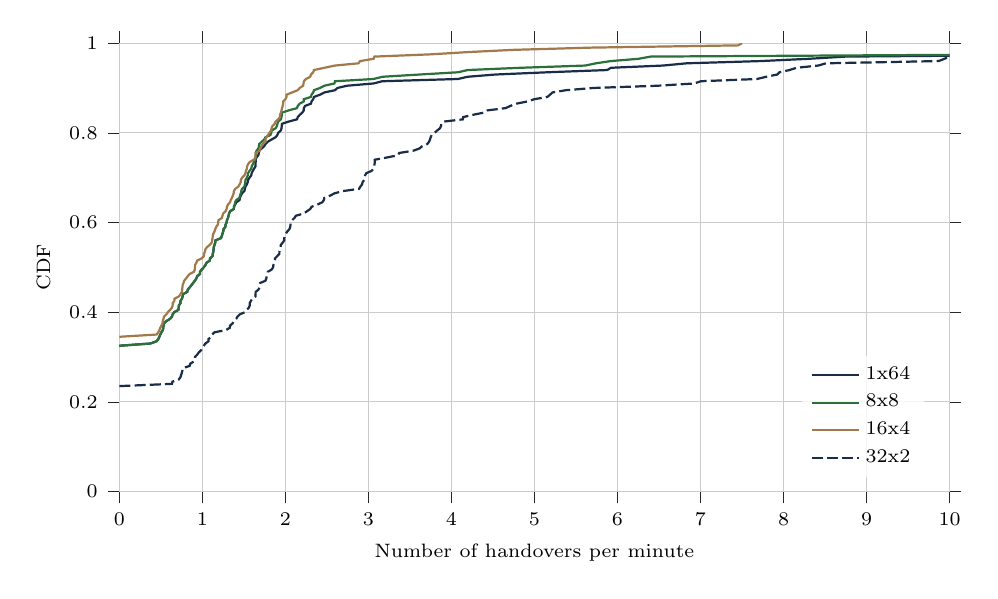
\begin{tikzpicture}

\definecolor{color0}{rgb}{0.0964154061637055,0.177286718595531,0.283473631853997}
\definecolor{color1}{rgb}{0.17004232121058,0.436797596475173,0.223725555555555}
\definecolor{color2}{rgb}{0.632842247501842,0.474798109622068,0.290702092080255}
\definecolor{color3}{rgb}{0.82995767878942,0.563202403524827,0.776274444444444}
\definecolor{color4}{rgb}{0.763267446283815,0.850242277575182,0.951553976205169}

\begin{axis}[
axis line style={white!80!black},
legend cell align={left},
legend style={fill opacity=0.8, draw opacity=1, text opacity=1, at={(0.97,0.03)}, anchor=south east, draw=none},
tick align=outside,
tick pos=both,
% title={h/t 40offset 3dB, update period 0.1s, height 40m},
x grid style={white!80!black},
xlabel={Number of handovers per minute},
xmajorgrids,
xmin=0, xmax=10,
xtick style={color=white!15!black},
y grid style={white!80!black},
ylabel={CDF},
ymajorgrids,
ymin=0, ymax=1,
ytick style={color=white!15!black}
]
\addplot [thick, color0]
table {%
0 0.325
0.374064837905248 0.33
0.448765893792083 0.335
0.469483568075128 0.34
0.481927710843384 0.345
0.492610837438434 0.35
0.505902192242843 0.355
0.523560209424094 0.36
0.529100529100539 0.365
0.531443755535883 0.37
0.53715308863027 0.375
0.564971751412439 0.38
0.611620795107042 0.385
0.632911392405071 0.39
0.641711229946531 0.395
0.662251655629145 0.4
0.710900473933678 0.405
0.714853057982554 0.41
0.716845878136205 0.415
0.736196319018408 0.42
0.736196319018434 0.425
0.752823086574657 0.43
0.762388818297334 0.435
0.765794511806021 0.44
0.817438692098123 0.445
0.823045267489735 0.45
0.846262341325834 0.455
0.868306801736636 0.46
0.8880118401579 0.465
0.909090909090902 0.47
0.927357032457487 0.475
0.937500000000022 0.48
0.970873786407805 0.485
0.971397733405321 0.49
0.991735537190073 0.495
1.01781170483463 0.5
1.0362694300518 0.505
1.04986876640422 0.51
1.08827085852482 0.515
1.09289617486341 0.52
1.12289457267627 0.525
1.12500000000003 0.53
1.1320754716981 0.535
1.13464447806358 0.54
1.13708149084021 0.545
1.14591291061883 0.55
1.15495668912418 0.555
1.15696104897806 0.56
1.22399020807838 0.565
1.23456790123458 0.57
1.24172185430468 0.575
1.25130344108448 0.58
1.25457396759022 0.585
1.27659574468087 0.59
1.27931769722816 0.595
1.29124820659975 0.6
1.29589632829373 0.605
1.30832969908422 0.61
1.3148283418554 0.615
1.32207124495045 0.62
1.33333333333332 0.625
1.37931034482758 0.63
1.37983901878119 0.635
1.39534883720935 0.64
1.40845070422538 0.645
1.4475271411339 0.65
1.45278450363198 0.655
1.46341463414633 0.66
1.47783251231526 0.665
1.50564617314931 0.67
1.51196976060485 0.675
1.51898734177214 0.68
1.53583617747446 0.685
1.54639175257735 0.69
1.55038759689921 0.695
1.56794425087104 0.7
1.58850226928901 0.705
1.59386068476974 0.71
1.60734787600465 0.715
1.62162162162161 0.72
1.63934426229507 0.725
1.64083865086606 0.73
1.64158686730506 0.735
1.64183642444509 0.74
1.65238678090572 0.745
1.67389956602601 0.75
1.68067226890758 0.755
1.68539325842699 0.76
1.71428571428577 0.765
1.74418604651162 0.77
1.75953079178885 0.775
1.78748758689176 0.78
1.8339276617423 0.785
1.8808777429467 0.79
1.90325138778751 0.795
1.91311279394189 0.8
1.94489465153969 0.805
1.95333695062405 0.81
1.95599022004894 0.815
1.958224543081 0.82
2.03873598369012 0.825
2.13980028530676 0.83
2.14899713467053 0.835
2.17216411906686 0.84
2.20318237454107 0.845
2.2222222222222 0.85
2.22222222222228 0.855
2.23728813559323 0.86
2.3076923076923 0.865
2.31511254019299 0.87
2.33463035019454 0.875
2.34476769431186 0.88
2.41718889883626 0.885
2.46913580246913 0.89
2.59740259740259 0.895
2.62714718760526 0.9
2.74165202108967 0.905
3.06122448979592 0.91
3.1654676258994 0.915
4.07816482582846 0.92
4.19580419580421 0.925
4.53001132502845 0.93
5.15672396359978 0.935
5.87570621468944 0.940000000000001
5.92105263157892 0.945000000000001
6.54715510522229 0.950000000000001
6.83371298405492 0.955000000000001
7.72635814889367 0.960000000000001
8.29711576452028 0.965000000000001
8.74999999999993 0.970000000000001
12.1037463976944 0.975000000000001
15.4981549815497 0.980000000000001
16.0919540229884 0.985000000000001
40.9937888198755 0.990000000000001
68.2464454976302 0.995000000000001
82.5000000000002 1
};
\addlegendentry{1x64}
\addplot [thick, color1]
table {%
0 0.325
0.374064837905248 0.33
0.448765893792083 0.335
0.469483568075128 0.34
0.481927710843384 0.345
0.492610837438434 0.35
0.505902192242843 0.355
0.523560209424094 0.36
0.529100529100539 0.365
0.531443755535883 0.37
0.53715308863027 0.375
0.564971751412439 0.38
0.611620795107042 0.385
0.632911392405071 0.39
0.641711229946531 0.395
0.662251655629145 0.4
0.710900473933678 0.405
0.714853057982554 0.41
0.716845878136205 0.415
0.736196319018408 0.42
0.736196319018434 0.425
0.752823086574657 0.43
0.762388818297334 0.435
0.765794511806021 0.44
0.817438692098123 0.445
0.823045267489735 0.45
0.846262341325834 0.455
0.868306801736636 0.46
0.8880118401579 0.465
0.909090909090902 0.47
0.927357032457487 0.475
0.937500000000022 0.48
0.970873786407805 0.485
0.971397733405321 0.49
0.991735537190073 0.495
1.01781170483463 0.5
1.0362694300518 0.505
1.04986876640422 0.51
1.08827085852482 0.515
1.09289617486341 0.52
1.12289457267627 0.525
1.12500000000003 0.53
1.1320754716981 0.535
1.13464447806358 0.54
1.13708149084021 0.545
1.14591291061883 0.55
1.15495668912418 0.555
1.15696104897806 0.56
1.22399020807838 0.565
1.23456790123458 0.57
1.24172185430468 0.575
1.25130344108448 0.58
1.25457396759022 0.585
1.27659574468087 0.59
1.27931769722816 0.595
1.29124820659975 0.6
1.29589632829373 0.605
1.30832969908422 0.61
1.3148283418554 0.615
1.32207124495045 0.62
1.33333333333332 0.625
1.37931034482758 0.63
1.37983901878119 0.635
1.39026812313803 0.64
1.39534883720935 0.645
1.40845070422538 0.65
1.4475271411339 0.655
1.45278450363198 0.66
1.46341463414633 0.665
1.46878824969405 0.67
1.47783251231526 0.675
1.50564617314931 0.68
1.51196976060485 0.685
1.51668351870582 0.69
1.51898734177214 0.695
1.53583617747446 0.7
1.54639175257735 0.705
1.55038759689921 0.71
1.56794425087104 0.715
1.58850226928901 0.72
1.59386068476974 0.725
1.60734787600465 0.73
1.62162162162161 0.735
1.63934426229507 0.74
1.64083865086606 0.745
1.64158686730506 0.75
1.64183642444509 0.755
1.65238678090572 0.76
1.67389956602601 0.765
1.68067226890758 0.77
1.68539325842699 0.775
1.71428571428577 0.78
1.74418604651162 0.785
1.75953079178885 0.79
1.81879420680364 0.795
1.83050847457628 0.8
1.8339276617423 0.805
1.8808777429467 0.81
1.89806678383131 0.815
1.90325138778751 0.82
1.91311279394189 0.825
1.94489465153969 0.83
1.95333695062405 0.835
1.95599022004894 0.84
1.958224543081 0.845
2.03873598369012 0.85
2.13980028530676 0.855
2.14899713467053 0.86
2.17216411906686 0.865
2.2222222222222 0.87
2.22222222222228 0.875
2.3076923076923 0.88
2.31511254019299 0.885
2.33463035019454 0.89
2.34476769431186 0.895
2.41718889883626 0.9
2.46913580246913 0.905
2.58992805755405 0.91
2.59740259740259 0.915
3.06122448979592 0.92
3.17100792751992 0.925
3.61581920903966 0.93
4.07816482582846 0.935
4.19580419580421 0.940000000000001
4.82897384305854 0.945000000000001
5.61184723304768 0.950000000000001
5.74031890660614 0.955000000000001
5.92105263157892 0.960000000000001
6.24999999999995 0.965000000000001
6.40063216120136 0.970000000000001
11.070110701107 0.975000000000001
12.1037463976944 0.980000000000001
16.0919540229884 0.985000000000001
40.9937888198755 0.990000000000001
51.1848341232227 0.995000000000001
67.5000000000002 1
};
\addlegendentry{8x8}
\addplot [thick, color2]
table {%
0 0.345
0.448765893792083 0.35
0.469483568075128 0.355
0.481927710843384 0.36
0.492610837438434 0.365
0.505902192242843 0.37
0.519930675909889 0.375
0.523560209424094 0.38
0.531443755535883 0.385
0.53715308863027 0.39
0.564971751412439 0.395
0.584795321637436 0.4
0.611620795107042 0.405
0.632911392405071 0.41
0.641711229946531 0.415
0.642398286937909 0.42
0.662251655629145 0.425
0.66481994459836 0.43
0.716845878136205 0.435
0.736196319018408 0.44
0.752823086574657 0.445
0.756620428751599 0.45
0.759493670886078 0.455
0.762388818297334 0.46
0.771704180064331 0.465
0.781250000000001 0.47
0.802139037433178 0.475
0.823045267489735 0.48
0.846262341325834 0.485
0.897531787584166 0.49
0.909090909090902 0.495
0.909780136467043 0.5
0.910931174089101 0.505
0.927357032457487 0.51
0.937500000000022 0.515
0.991735537190073 0.52
1.01781170483463 0.525
1.01954120645712 0.53
1.03092783505157 0.535
1.0362694300518 0.54
1.05633802816903 0.545
1.08827085852482 0.55
1.113172541744 0.555
1.11731843575423 0.56
1.12289457267627 0.565
1.12429731417867 0.57
1.1320754716981 0.575
1.14591291061883 0.58
1.15495668912418 0.585
1.16580310880832 0.59
1.18530225207433 0.595
1.19165839126117 0.6
1.19284294234597 0.605
1.23456790123458 0.61
1.24172185430468 0.615
1.24999999999999 0.62
1.27931769722816 0.625
1.29124820659975 0.63
1.29589632829373 0.635
1.30832969908422 0.64
1.33333333333332 0.645
1.34128166915055 0.65
1.35669869983046 0.655
1.36674259681098 0.66
1.37614678899084 0.665
1.37931034482758 0.67
1.39534883720935 0.675
1.43312101910831 0.68
1.44810941271124 0.685
1.46163215590749 0.69
1.46341463414633 0.695
1.47783251231526 0.7
1.50564617314931 0.705
1.51898734177214 0.71
1.52413209144796 0.715
1.53583617747446 0.72
1.53846153846154 0.725
1.55038759689921 0.73
1.57068062827225 0.735
1.62162162162161 0.74
1.63934426229507 0.745
1.64083865086606 0.75
1.64158686730506 0.755
1.68855534709196 0.76
1.69971671388101 0.765
1.7094017094017 0.77
1.72910662824206 0.775
1.75953079178885 0.78
1.75953079178891 0.785
1.76991150442481 0.79
1.79015415216317 0.795
1.80722891566264 0.8
1.82717929196809 0.805
1.83299389002038 0.81
1.84426229508199 0.815
1.87061574434923 0.82
1.8808777429467 0.825
1.91311279394189 0.83
1.93409742120347 0.835
1.93548387096779 0.84
1.94489465153969 0.845
1.95333695062405 0.85
1.96721311475408 0.86
1.97260273972609 0.865
1.97368421052631 0.87
1.99999999999998 0.875
2.01342281879196 0.88
2.01438848920871 0.885
2.07972270363949 0.89
2.14861235452112 0.895
2.17216411906686 0.9
2.21402214022139 0.905
2.21811460258778 0.91
2.2222222222222 0.915
2.24719101123593 0.92
2.29885057471263 0.925
2.3076923076923 0.93
2.33463035019454 0.935
2.34476769431186 0.940000000000001
2.46913580246913 0.945000000000001
2.59740259740259 0.950000000000001
2.87999999999997 0.955000000000001
2.9001074113857 0.960000000000001
3.06122448979592 0.965000000000001
3.0729833546735 0.970000000000001
3.75000000000001 0.975000000000001
4.19580419580421 0.980000000000001
4.74683544303793 0.985000000000001
5.68720379146919 0.990000000000001
7.45341614906828 0.995000000000001
7.50000000000002 1
};
\addlegendentry{16x4}
% \addplot [thick, color3]
% table {%
% 0 0.325
% 0.374064837905248 0.33
% 0.448765893792083 0.335
% 0.469483568075128 0.34
% 0.481927710843384 0.345
% 0.492610837438434 0.35
% 0.505902192242843 0.355
% 0.523560209424094 0.36
% 0.529100529100539 0.365
% 0.531443755535883 0.37
% 0.53715308863027 0.375
% 0.564971751412439 0.38
% 0.611620795107042 0.385
% 0.632911392405071 0.39
% 0.641711229946531 0.395
% 0.662251655629145 0.4
% 0.710900473933678 0.405
% 0.714853057982554 0.41
% 0.716845878136205 0.415
% 0.736196319018408 0.42
% 0.736196319018434 0.425
% 0.752823086574657 0.43
% 0.762388818297334 0.435
% 0.765794511806021 0.44
% 0.817438692098123 0.445
% 0.823045267489735 0.45
% 0.846262341325834 0.455
% 0.868306801736636 0.46
% 0.8880118401579 0.465
% 0.909090909090902 0.47
% 0.927357032457487 0.475
% 0.937500000000022 0.48
% 0.970873786407805 0.485
% 0.971397733405321 0.49
% 0.991735537190073 0.495
% 1.01781170483463 0.5
% 1.0362694300518 0.505
% 1.04986876640422 0.51
% 1.08827085852482 0.515
% 1.09289617486341 0.52
% 1.12289457267627 0.525
% 1.12500000000003 0.53
% 1.1320754716981 0.535
% 1.13464447806358 0.54
% 1.13708149084021 0.545
% 1.14591291061883 0.55
% 1.15495668912418 0.555
% 1.15696104897806 0.56
% 1.22399020807838 0.565
% 1.23456790123458 0.57
% 1.24172185430468 0.575
% 1.25130344108448 0.58
% 1.25457396759022 0.585
% 1.27659574468087 0.59
% 1.27931769722816 0.595
% 1.29124820659975 0.6
% 1.29589632829373 0.605
% 1.30832969908422 0.61
% 1.3148283418554 0.615
% 1.32207124495045 0.62
% 1.33333333333332 0.625
% 1.37931034482758 0.63
% 1.37983901878119 0.635
% 1.39026812313803 0.64
% 1.39534883720935 0.645
% 1.40845070422538 0.65
% 1.4475271411339 0.655
% 1.45278450363198 0.66
% 1.46341463414633 0.665
% 1.46878824969405 0.67
% 1.47783251231526 0.675
% 1.50564617314931 0.68
% 1.51196976060485 0.685
% 1.51668351870582 0.69
% 1.51898734177214 0.695
% 1.53583617747446 0.7
% 1.54639175257735 0.705
% 1.55038759689921 0.71
% 1.56794425087104 0.715
% 1.58850226928901 0.72
% 1.59386068476974 0.725
% 1.60734787600465 0.73
% 1.62162162162161 0.735
% 1.63934426229507 0.74
% 1.64083865086606 0.745
% 1.64158686730506 0.75
% 1.64183642444509 0.755
% 1.65238678090572 0.76
% 1.67389956602601 0.765
% 1.68067226890758 0.77
% 1.68539325842699 0.775
% 1.71428571428577 0.78
% 1.74418604651162 0.785
% 1.75953079178885 0.79
% 1.81879420680364 0.795
% 1.83050847457628 0.8
% 1.8339276617423 0.805
% 1.8808777429467 0.81
% 1.89806678383131 0.815
% 1.90325138778751 0.82
% 1.91311279394189 0.825
% 1.94489465153969 0.83
% 1.95333695062405 0.835
% 1.95599022004894 0.84
% 1.958224543081 0.845
% 2.03873598369012 0.85
% 2.13980028530676 0.855
% 2.14899713467053 0.86
% 2.17216411906686 0.865
% 2.2222222222222 0.87
% 2.22222222222228 0.875
% 2.3076923076923 0.88
% 2.31511254019299 0.885
% 2.33463035019454 0.89
% 2.34476769431186 0.895
% 2.41718889883626 0.9
% 2.46913580246913 0.905
% 2.58992805755405 0.91
% 2.59740259740259 0.915
% 3.06122448979592 0.92
% 3.17100792751992 0.925
% 3.61581920903966 0.93
% 4.07816482582846 0.935
% 4.19580419580421 0.940000000000001
% 4.82897384305854 0.945000000000001
% 5.61184723304768 0.950000000000001
% 5.74031890660614 0.955000000000001
% 5.92105263157892 0.960000000000001
% 6.24999999999995 0.965000000000001
% 6.40063216120136 0.970000000000001
% 11.070110701107 0.975000000000001
% 12.1037463976944 0.980000000000001
% 16.0919540229884 0.985000000000001
% 40.9937888198755 0.990000000000001
% 51.1848341232227 0.995000000000001
% 67.5000000000002 1
% };
% \addlegendentry{32x2}
% \addplot [thick, color4]
% table {%
% 0 0.325
% 0.374064837905248 0.33
% 0.448765893792083 0.335
% 0.469483568075128 0.34
% 0.481927710843384 0.345
% 0.492610837438434 0.35
% 0.505902192242843 0.355
% 0.523560209424094 0.36
% 0.529100529100539 0.365
% 0.531443755535883 0.37
% 0.53715308863027 0.375
% 0.564971751412439 0.38
% 0.611620795107042 0.385
% 0.632911392405071 0.39
% 0.641711229946531 0.395
% 0.662251655629145 0.4
% 0.710900473933678 0.405
% 0.714853057982554 0.41
% 0.716845878136205 0.415
% 0.736196319018408 0.42
% 0.736196319018434 0.425
% 0.752823086574657 0.43
% 0.762388818297334 0.435
% 0.765794511806021 0.44
% 0.817438692098123 0.445
% 0.823045267489735 0.45
% 0.846262341325834 0.455
% 0.868306801736636 0.46
% 0.8880118401579 0.465
% 0.909090909090902 0.47
% 0.927357032457487 0.475
% 0.937500000000022 0.48
% 0.970873786407805 0.485
% 0.971397733405321 0.49
% 0.991735537190073 0.495
% 1.01781170483463 0.5
% 1.0362694300518 0.505
% 1.04986876640422 0.51
% 1.08827085852482 0.515
% 1.09289617486341 0.52
% 1.12289457267627 0.525
% 1.12500000000003 0.53
% 1.1320754716981 0.535
% 1.13464447806358 0.54
% 1.13708149084021 0.545
% 1.14591291061883 0.55
% 1.15495668912418 0.555
% 1.15696104897806 0.56
% 1.22399020807838 0.565
% 1.23456790123458 0.57
% 1.24172185430468 0.575
% 1.25130344108448 0.58
% 1.25457396759022 0.585
% 1.27659574468087 0.59
% 1.27931769722816 0.595
% 1.29124820659975 0.6
% 1.29589632829373 0.605
% 1.30832969908422 0.61
% 1.3148283418554 0.615
% 1.32207124495045 0.62
% 1.33333333333332 0.625
% 1.37931034482758 0.63
% 1.37983901878119 0.635
% 1.39026812313803 0.64
% 1.39534883720935 0.645
% 1.40845070422538 0.65
% 1.4475271411339 0.655
% 1.45278450363198 0.66
% 1.46341463414633 0.665
% 1.46878824969405 0.67
% 1.47783251231526 0.675
% 1.50564617314931 0.68
% 1.51196976060485 0.685
% 1.51668351870582 0.69
% 1.51898734177214 0.695
% 1.53583617747446 0.7
% 1.54639175257735 0.705
% 1.55038759689921 0.71
% 1.56794425087104 0.715
% 1.58850226928901 0.72
% 1.59386068476974 0.725
% 1.60734787600465 0.73
% 1.62162162162161 0.735
% 1.63934426229507 0.74
% 1.64083865086606 0.745
% 1.64158686730506 0.75
% 1.64183642444509 0.755
% 1.65238678090572 0.76
% 1.67389956602601 0.765
% 1.68067226890758 0.77
% 1.68539325842699 0.775
% 1.71428571428577 0.78
% 1.74418604651162 0.785
% 1.75953079178885 0.79
% 1.81879420680364 0.795
% 1.83050847457628 0.8
% 1.8339276617423 0.805
% 1.8808777429467 0.81
% 1.89806678383131 0.815
% 1.90325138778751 0.82
% 1.91311279394189 0.825
% 1.94489465153969 0.83
% 1.95333695062405 0.835
% 1.95599022004894 0.84
% 1.958224543081 0.845
% 2.03873598369012 0.85
% 2.13980028530676 0.855
% 2.14899713467053 0.86
% 2.17216411906686 0.865
% 2.2222222222222 0.87
% 2.22222222222228 0.875
% 2.3076923076923 0.88
% 2.31511254019299 0.885
% 2.33463035019454 0.89
% 2.34476769431186 0.895
% 2.41718889883626 0.9
% 2.46913580246913 0.905
% 2.58992805755405 0.91
% 2.59740259740259 0.915
% 3.06122448979592 0.92
% 3.17100792751992 0.925
% 4.06779661016962 0.93
% 4.07816482582846 0.935
% 4.19580419580421 0.940000000000001
% 5.3118712273644 0.945000000000001
% 5.61184723304768 0.950000000000001
% 5.92105263157892 0.955000000000001
% 6.24999999999995 0.960000000000001
% 6.28701594533053 0.965000000000001
% 6.87475306203109 0.970000000000001
% 11.070110701107 0.975000000000001
% 12.1037463976944 0.980000000000001
% 16.0919540229884 0.985000000000001
% 40.9937888198755 0.990000000000001
% 56.8720379146919 0.995000000000001
% 82.5000000000002 1
% };
% \addlegendentry{64x1}
\addplot [thick, color0, dash pattern=on 4pt off 1.5pt]
table {%
0 0.235
0.632911392405071 0.24
0.63965884861408 0.245
0.716845878136205 0.25
0.736196319018408 0.255
0.752823086574657 0.265
0.759493670886078 0.27
0.762388818297334 0.275
0.846262341325834 0.28
0.854700854700851 0.285
0.897531787584166 0.29
0.909090909090902 0.295
0.910931174089101 0.3
0.937500000000022 0.305
0.955414012738875 0.31
0.985221674876869 0.315
0.993377483443747 0.32
1.01781170483463 0.325
1.0362694300518 0.33
1.07334525939176 0.335
1.07430617726054 0.34
1.10905730129389 0.345
1.11731843575423 0.35
1.14591291061883 0.355
1.28342245989306 0.36
1.32963988919672 0.365
1.33333333333332 0.37
1.36467020470056 0.375
1.37931034482758 0.38
1.40845070422538 0.385
1.42236270248919 0.39
1.45102781136643 0.395
1.5132408575032 0.4
1.53583617747446 0.405
1.55979202772967 0.41
1.57068062827225 0.415
1.57068062827228 0.42
1.58450704225355 0.425
1.6 0.43
1.63934426229507 0.435
1.64083865086606 0.44
1.64158686730506 0.445
1.67441860465122 0.45
1.68855534709196 0.455
1.68946098149645 0.46
1.69491525423728 0.465
1.75953079178885 0.47
1.76991150442481 0.475
1.77514792899407 0.48
1.78571428571427 0.485
1.78837555886741 0.49
1.83486238532113 0.495
1.85185185185188 0.5
1.85528756957334 0.505
1.87149095446044 0.51
1.87382885696445 0.515
1.87499999999998 0.52
1.90174326465925 0.525
1.92719486081373 0.53
1.92771084337354 0.535
1.93548387096773 0.54
1.94300518134721 0.545
1.94489465153969 0.55
1.96721311475408 0.555
1.98609731876862 0.56
1.98675496688744 0.565
1.99004975124376 0.57
2.00534759358294 0.575
2.02360876897137 0.58
2.04778156996586 0.585
2.05761316872434 0.59
2.06185567010313 0.595
2.06422018348625 0.6
2.07972270363949 0.605
2.10896309314585 0.61
2.12577502214353 0.615
2.2222222222222 0.62
2.25988700564975 0.625
2.29885057471263 0.63
2.31511254019299 0.635
2.38568588469193 0.64
2.4439918533605 0.645
2.46334310850448 0.65
2.46913580246913 0.655
2.54022015241326 0.66
2.59179265658745 0.665
2.6925953627525 0.67
2.88739172281044 0.675
2.90322580645168 0.68
2.92397660818718 0.685
2.93000542593607 0.69
2.95081967213112 0.695
2.95566502463055 0.7
2.95890410958914 0.705
2.97520661157022 0.71
3.03797468354428 0.715
3.06122448979592 0.72
3.06905370843988 0.725
3.07377049180332 0.73
3.07692307692308 0.735
3.07692307692308 0.74
3.2258064516129 0.745
3.35570469798661 0.75
3.3707865168539 0.755
3.53982300884954 0.76
3.61445783132528 0.765
3.647416413374 0.77
3.70942812982995 0.775
3.73092142453376 0.78
3.74100719424474 0.785
3.75000000000001 0.79
3.76175548589339 0.795
3.79746835443034 0.8
3.82687927107076 0.805
3.86162510056331 0.81
3.87374461979924 0.815000000000001
3.87866732968686 0.820000000000001
3.90625 0.825000000000001
4.13793103448277 0.830000000000001
4.14129110840455 0.835000000000001
4.25531914893618 0.840000000000001
4.39024390243899 0.845000000000001
4.43349753694578 0.850000000000001
4.65116279069764 0.855000000000001
4.70998691670319 0.860000000000001
4.78278198485471 0.865000000000001
4.91803278688523 0.870000000000001
4.99999999999996 0.875000000000001
5.15574650913014 0.880000000000001
5.18731988472619 0.885000000000001
5.21739130434781 0.890000000000001
5.37772087067863 0.895000000000001
5.70993528740027 0.900000000000001
6.48648648648644 0.905000000000001
6.9230769230769 0.910000000000001
7.00389105058363 0.915000000000001
7.67999999999992 0.920000000000001
7.79220779220777 0.925000000000001
7.92452830188672 0.930000000000001
7.95128939828094 0.935000000000001
8.07174887892375 0.940000000000001
8.15632965165692 0.945000000000001
8.41777084957151 0.950000000000001
8.51063829787236 0.955000000000001
9.86842105263153 0.960000000000001
9.93733213966018 0.965000000000001
9.9999999999999 0.970000000000001
11.25 0.975000000000001
11.3744075829384 0.980000000000001
14.9068322981366 0.985000000000001
17.7121771217711 0.990000000000001
20.979020979021 0.995000000000001
41.3793103448276 1
};
\addlegendentry{32x2}
% \addplot [semithick, color0, dash pattern=on 4pt off 1.5pt]
% table {%
% 0 0.3
% 0.469483568075128 0.305
% 0.505902192242843 0.31
% 0.523560209424094 0.315
% 0.611620795107042 0.32
% 0.632911392405071 0.325
% 0.642398286937909 0.33
% 0.662251655629145 0.335
% 0.716845878136205 0.34
% 0.736196319018408 0.345
% 0.752823086574657 0.355
% 0.759493670886078 0.36
% 0.762388818297334 0.365
% 0.781250000000001 0.37
% 0.894632206759475 0.375
% 0.897531787584166 0.38
% 0.909090909090902 0.385
% 0.909780136467043 0.39
% 0.910931174089101 0.395
% 0.927357032457487 0.4
% 0.937500000000022 0.405
% 0.955414012738875 0.41
% 0.985221674876869 0.415
% 0.991735537190073 0.42
% 0.993377483443747 0.425
% 0.99722991689754 0.43
% 1.01781170483463 0.435
% 1.0362694300518 0.44
% 1.03986135181978 0.445
% 1.06288751107177 0.45
% 1.10905730129389 0.455
% 1.11731843575423 0.46
% 1.12570356472797 0.465
% 1.12994350282488 0.47
% 1.1349306431274 0.475
% 1.14591291061883 0.48
% 1.15495668912418 0.485
% 1.16580310880832 0.49
% 1.16959064327487 0.495
% 1.20675784392603 0.5
% 1.26939351198875 0.505
% 1.27931769722816 0.51
% 1.28342245989306 0.515
% 1.29589632829373 0.52
% 1.33333333333332 0.525
% 1.34629768137625 0.53
% 1.36736554238838 0.535
% 1.37931034482758 0.54
% 1.42236270248919 0.545
% 1.44578313253015 0.55
% 1.45102781136643 0.555
% 1.47783251231528 0.56
% 1.49906308557156 0.565
% 1.52413209144796 0.57
% 1.53583617747446 0.575
% 1.54340836012866 0.58
% 1.54639175257735 0.585
% 1.57068062827225 0.59
% 1.58450704225355 0.595
% 1.6 0.6
% 1.60427807486636 0.605
% 1.63934426229507 0.61
% 1.64158686730506 0.615
% 1.64609053497947 0.62
% 1.67441860465122 0.625
% 1.7052375152254 0.63
% 1.7094017094017 0.635
% 1.75953079178885 0.64
% 1.76991150442481 0.645
% 1.77514792899407 0.65
% 1.83299389002038 0.655
% 1.84426229508199 0.66
% 1.85528756957334 0.665
% 1.87149095446044 0.67
% 1.87499999999998 0.675
% 1.90174326465925 0.68
% 1.93548387096779 0.685
% 1.94489465153969 0.69
% 1.96721311475408 0.695
% 1.98609731876862 0.7
% 2.01342281879196 0.705
% 2.06422018348625 0.71
% 2.07972270363949 0.715
% 2.08423795049943 0.72
% 2.2222222222222 0.725
% 2.23546944858426 0.73
% 2.27889310906139 0.735
% 2.29885057471263 0.74
% 2.46913580246913 0.745
% 2.49999999999998 0.75
% 2.63013698630146 0.755
% 2.68523122824475 0.76
% 2.71339739966091 0.765
% 2.73348519362197 0.77
% 2.81524926686226 0.775
% 2.84810126582276 0.78
% 2.87769784172672 0.785
% 2.95081967213112 0.79
% 2.95566502463052 0.795
% 3.03797468354428 0.8
% 3.06122448979592 0.805
% 3.0729833546735 0.81
% 3.07692307692308 0.815
% 3.08641975308646 0.82
% 3.13999127780213 0.825
% 3.2258064516129 0.83
% 3.3707865168539 0.835
% 3.39622641509431 0.84
% 3.61445783132528 0.845
% 3.6202735317781 0.85
% 3.76175548589339 0.855
% 3.83999999999996 0.86
% 3.86819484240695 0.865
% 3.87374461979924 0.87
% 3.88275599543218 0.875
% 4.06536468712651 0.88
% 4.13793103448277 0.885
% 4.18904403866824 0.89
% 4.25531914893618 0.895
% 4.39024390243899 0.9
% 4.65116279069764 0.905
% 5.09770603228558 0.91
% 5.18731988472619 0.915
% 5.21739130434781 0.92
% 5.3811659192825 0.925
% 5.68720379146919 0.93
% 5.92105263157892 0.935
% 6.07950116913498 0.940000000000001
% 6.48648648648644 0.945000000000001
% 6.7144136078785 0.950000000000001
% 6.9230769230769 0.955000000000001
% 6.99999999999993 0.960000000000001
% 7.00389105058363 0.965000000000001
% 7.79220779220777 0.970000000000001
% 8.51063829787236 0.975000000000001
% 11.070110701107 0.980000000000001
% 11.25 0.985000000000001
% 12.5874125874126 0.990000000000001
% 14.9068322981366 0.995000000000001
% 20.6896551724138 1
% };
% \addlegendentry{8x2}
% \addplot [semithick, color1, dash pattern=on 4pt off 1.5pt]
% table {%
% 0 0.26
% 0.448765893792083 0.265
% 0.469483568075128 0.27
% 0.505902192242843 0.275
% 0.519930675909889 0.28
% 0.523560209424094 0.285
% 0.611620795107042 0.29
% 0.632911392405071 0.295
% 0.642398286937909 0.3
% 0.662251655629145 0.305
% 0.66481994459836 0.31
% 0.716845878136205 0.315
% 0.725513905683215 0.32
% 0.736196319018408 0.325
% 0.752823086574657 0.335
% 0.756620428751599 0.34
% 0.759493670886078 0.345
% 0.762388818297334 0.35
% 0.771704180064331 0.355
% 0.781250000000001 0.36
% 0.8 0.365
% 0.802139037433178 0.37
% 0.823045267489735 0.375
% 0.897531787584166 0.38
% 0.909780136467043 0.385
% 0.910931174089101 0.39
% 0.937500000000022 0.395
% 0.943396226415085 0.4
% 0.950871632329626 0.405
% 0.963855421686769 0.41
% 0.985221674876869 0.415
% 0.993377483443747 0.42
% 1.01781170483463 0.425
% 1.0362694300518 0.43
% 1.03986135181975 0.435
% 1.06288751107177 0.44
% 1.10905730129389 0.445
% 1.113172541744 0.45
% 1.11731843575423 0.455
% 1.12289457267627 0.46
% 1.12429731417867 0.465
% 1.12570356472797 0.47
% 1.12994350282488 0.475
% 1.16959064327487 0.48
% 1.19284294234597 0.485
% 1.26939351198875 0.49
% 1.27931769722816 0.495
% 1.28342245989306 0.5
% 1.29589632829373 0.505
% 1.33333333333332 0.51
% 1.34128166915055 0.515
% 1.35440180586906 0.52
% 1.36736554238838 0.525
% 1.3750954927426 0.53
% 1.37614678899084 0.535
% 1.37931034482758 0.54
% 1.39026812313803 0.545
% 1.42236270248919 0.55
% 1.43312101910831 0.555
% 1.47783251231528 0.56
% 1.52413209144796 0.565
% 1.53452685421994 0.57
% 1.54639175257735 0.575
% 1.55440414507777 0.58
% 1.57068062827225 0.585
% 1.61145926589081 0.59
% 1.62778079218671 0.595
% 1.64158686730506 0.6
% 1.67441860465122 0.605
% 1.68946098149645 0.61
% 1.69971671388101 0.615
% 1.7094017094017 0.62
% 1.73243503368626 0.625
% 1.75953079178885 0.63
% 1.75953079178891 0.635
% 1.76991150442481 0.64
% 1.77514792899407 0.645
% 1.79180887372021 0.65
% 1.83486238532109 0.655
% 1.84426229508199 0.66
% 1.87499999999998 0.665
% 1.93548387096779 0.67
% 1.94884287454332 0.675
% 1.96721311475408 0.685
% 1.98347107438015 0.69
% 2.01342281879196 0.695
% 2.03504804974569 0.7
% 2.08423795049943 0.705
% 2.08851317752369 0.71
% 2.09332751853475 0.715
% 2.11267605633807 0.72
% 2.15225189318462 0.725
% 2.21402214022139 0.73
% 2.24032586558046 0.735
% 2.24719101123593 0.74
% 2.29885057471263 0.745
% 2.30215827338138 0.75
% 2.30769230769231 0.755
% 2.41351568785207 0.76
% 2.60869565217391 0.765
% 2.78207109737246 0.77
% 2.79369627507168 0.775
% 2.87081339712918 0.78
% 2.91734197730953 0.785
% 2.95566502463052 0.79
% 2.95890410958914 0.795
% 3.00683371298417 0.8
% 3.0729833546735 0.805
% 3.08641975308646 0.81
% 3.22234156820634 0.815000000000001
% 3.24324324324322 0.820000000000001
% 3.3333333333333 0.825000000000001
% 3.61445783132528 0.830000000000001
% 3.65435858393617 0.835000000000001
% 3.74123148869845 0.840000000000001
% 3.79746835443034 0.845000000000001
% 3.83999999999996 0.850000000000001
% 3.87096774193546 0.855000000000001
% 3.99999999999996 0.860000000000001
% 4.25531914893618 0.865000000000001
% 4.30416068866582 0.870000000000001
% 4.52830188679241 0.875000000000001
% 4.56580125335738 0.880000000000001
% 4.58793542905702 0.885000000000001
% 4.6153846153846 0.890000000000001
% 4.99999999999996 0.895000000000001
% 5.18731988472619 0.900000000000001
% 5.3811659192825 0.905000000000001
% 6.07594936708856 0.910000000000001
% 6.12244897959183 0.915000000000001
% 6.20155038759686 0.920000000000001
% 6.45161290322581 0.925000000000001
% 6.55737704918028 0.930000000000001
% 7.00389105058363 0.935000000000001
% 7.40740740740738 0.940000000000001
% 7.52351097178679 0.945000000000001
% 7.79220779220777 0.950000000000001
% 7.89473684210522 0.955000000000001
% 8.39160839160841 0.960000000000001
% 8.51063829787236 0.965000000000001
% 8.78048780487798 0.970000000000001
% 10.5263157894737 0.975000000000001
% 11.070110701107 0.980000000000001
% 18.75 0.985000000000001
% 22.7488151658767 0.990000000000001
% 27.950310559006 0.995000000000001
% 41.3793103448276 1
% };
% \addlegendentry{16x2}

\end{axis}

\end{tikzpicture}

% \caption{Cumulative distribution function plot of the number of handovers per minute for different antenna array topologies of a total of 64 antenna elements at an altitude of $40$~m.}
% \label{fig:handovers40_2}
% \end{figure}
% \begin{figure}[tbp]
% \centering
% % \centerline{
% % \includegraphics{handover_per_min}
% % }
% \include{handover_per_min40}
% \caption{Cumulative distribution function plot of the number of handovers per minute for different antenna array topologies of a total of 256 antenna elements at an altitude of $40$~m.}
% \label{fig:handovers40}
% \end{figure}
\par Figure~\ref{fig:handovers150} shows the same results as previous figure, but for UAVs flying at an altitude of $150$~m above ground level. We can conclude that the effect of the different antenna topologies is significantly less at an altitude of $150$~m. This can be explained by the fact that users have a larger distance towards the BS, thus the angular movement of the users is significantly less, which results in reduced beamtracking requirements.

\begin{figure}[tbp]
\centering
% \centerline{
% \includegraphics{handover_per_min}
% }
% This file was created by tikzplotlib v0.9.3.
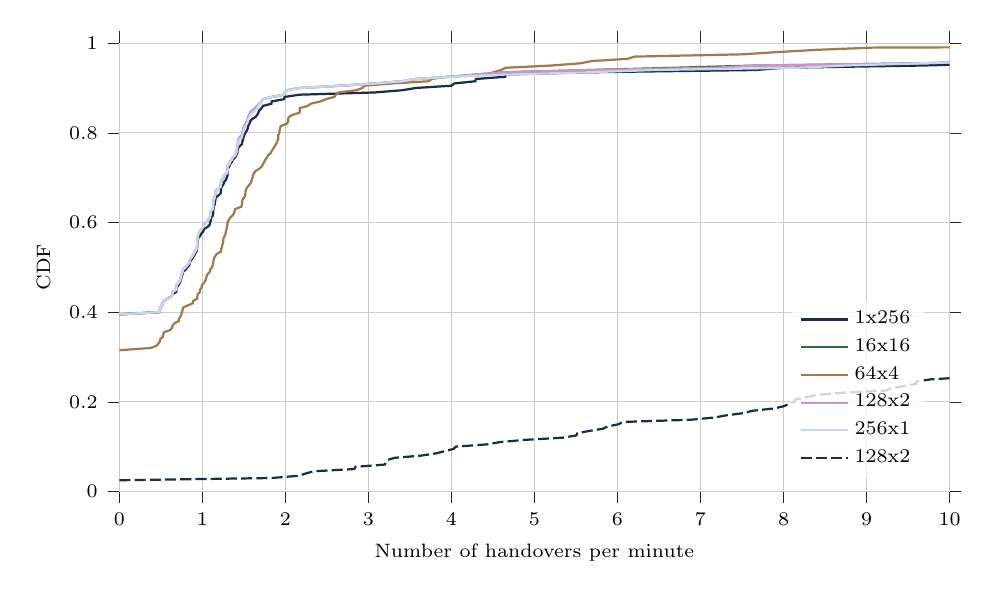
\begin{tikzpicture}

% \definecolor{color0}{rgb}{0.298039215686275,0.447058823529412,0.690196078431373}
% \definecolor{color1}{rgb}{0.866666666666667,0.517647058823529,0.32156862745098}
% \definecolor{color2}{rgb}{0.333333333333333,0.658823529411765,0.407843137254902}
% \definecolor{color3}{rgb}{0.768627450980392,0.305882352941176,0.32156862745098}
% \definecolor{color4}{rgb}{0.505882352941176,0.447058823529412,0.701960784313725}
\definecolor{color0}{rgb}{0.0964154061637055,0.177286718595531,0.283473631853997}
\definecolor{color1}{rgb}{0.17004232121058,0.436797596475173,0.223725555555555}
\definecolor{color2}{rgb}{0.632842247501842,0.474798109622068,0.290702092080255}
\definecolor{color3}{rgb}{0.82995767878942,0.563202403524827,0.776274444444444}
\definecolor{color4}{rgb}{0.763267446283815,0.850242277575182,0.951553976205169}

\begin{axis}[
axis line style={white!80!black},
legend cell align={left},
legend style={fill opacity=0.8, draw opacity=1, text opacity=1, at={(0.97,0.03)}, anchor=south east, draw=none},
tick align=outside,
tick pos=both,
% title={h/t 40offset 3dB, update period 0.1s, height 40m},
x grid style={white!80!black},
xlabel={Number of handovers per minute},
xmajorgrids,
xmin=0, xmax=10,
xtick style={color=white!15!black},
y grid style={white!80!black},
ylabel={CDF},
ymajorgrids,
ymin=0, ymax=1,
ytick style={color=white!15!black}
]
\addplot [thick, color0]
table {%
0 0.395
0.481927710843384 0.4
0.488997555012236 0.405
0.490797546012289 0.41
0.509770603228558 0.415
0.523560209424094 0.42
0.53715308863027 0.425
0.577478344562088 0.43
0.625651720542239 0.435
0.63965884861408 0.44
0.685714285714308 0.445
0.688863375430564 0.45
0.689919509390595 0.455
0.711181351244596 0.46
0.728155339805854 0.465
0.736196319018408 0.47
0.752823086574657 0.48
0.762388818297334 0.485
0.767918088737231 0.49
0.8 0.495
0.817438692098123 0.5
0.843585237258359 0.505
0.846262341325834 0.51
0.860832137733164 0.515
0.879765395894423 0.52
0.897531787584166 0.525
0.91001011122349 0.53
0.927357032457487 0.535
0.935307872174613 0.54
0.937499999999991 0.545
0.937500000000022 0.55
0.938967136150257 0.555
0.943396226415085 0.56
0.950871632329626 0.565
0.972447325769844 0.57
0.985221674876869 0.575
1.01180438448569 0.58
1.01781170483463 0.585
1.06288751107177 0.59
1.08827085852482 0.595
1.09455761629673 0.6
1.10159118727048 0.605
1.10172603745871 0.61
1.12500000000003 0.615
1.12994350282488 0.62
1.12994350282489 0.625
1.13464447806358 0.63
1.13708149084021 0.635
1.14869176770903 0.64
1.15107913669069 0.645
1.15696104897806 0.65
1.1575562700965 0.655
1.19165839126117 0.66
1.21951219512192 0.665
1.22324159021407 0.67
1.22324159021408 0.675
1.23456790123458 0.68
1.25457396759022 0.685
1.26050420168069 0.69
1.28342245989306 0.695
1.29519697787376 0.7
1.30222463374937 0.705
1.30246020260495 0.71
1.30264871906214 0.715
1.30832969908422 0.72
1.32450331125829 0.725
1.33333333333337 0.73
1.35440180586906 0.735
1.36736554238838 0.74
1.39534883720935 0.745
1.40845070422538 0.75
1.42180094786736 0.755
1.42372881355933 0.76
1.42743854084064 0.765
1.44869215291756 0.77
1.47783251231526 0.775
1.4800197335965 0.78
1.49006622516562 0.785
1.49625935162099 0.79
1.50429799426937 0.795
1.51898734177214 0.8
1.53452685421994 0.805
1.54639175257735 0.81
1.55038759689921 0.815
1.5665796344648 0.82
1.57480314960633 0.825
1.59386068476974 0.83
1.63934426229507 0.835
1.66032514700797 0.84
1.67397369469915 0.845
1.68539325842699 0.85
1.71358629130974 0.855
1.72910662824206 0.86
1.83346065699013 0.865
1.83486238532109 0.87
1.98347107438015 0.875
1.99004975124376 0.88
2.17129071170086 0.885
3.07692307692308 0.89
3.40909090909091 0.895
3.57142857142855 0.9
4.00000000000001 0.905
4.03191936161292 0.91
4.28911834789533 0.915
4.29338103756704 0.92
4.64802963960931 0.925
4.64972101673893 0.93
5.66037735849058 0.935
7.66062602965434 0.940000000000001
7.99999999999994 0.945000000000001
9.66875559534504 0.950000000000001
10.6487148102818 0.955000000000001
10.6995884773665 0.960000000000001
14.2439737034335 0.965000000000001
14.550641940086 0.970000000000001
15.6285390713482 0.975000000000001
15.9574468085109 0.980000000000001
16.3388804841155 0.985000000000001
17.1359613837497 0.990000000000001
19.6810933940782 0.995000000000001
26.9494697442304 1
};
\addlegendentry{1x256}
\addplot [thick, color1]
table {%
0 0.395
0.481927710843384 0.4
0.488997555012236 0.405
0.490797546012289 0.41
0.509770603228558 0.415
0.523560209424094 0.42
0.53715308863027 0.425
0.577478344562088 0.43
0.625651720542239 0.435
0.63965884861408 0.44
0.641711229946531 0.445
0.685714285714308 0.45
0.688863375430564 0.455
0.689919509390595 0.46
0.711181351244596 0.465
0.728155339805854 0.47
0.736196319018408 0.475
0.752823086574657 0.485
0.762388818297334 0.49
0.767918088737231 0.495
0.8 0.5
0.817438692098123 0.505
0.843585237258359 0.51
0.846262341325834 0.515
0.860832137733164 0.52
0.879765395894423 0.525
0.897531787584166 0.53
0.91001011122349 0.535
0.927357032457487 0.54
0.935307872174613 0.545
0.937499999999991 0.55
0.937500000000022 0.555
0.938967136150257 0.56
0.943396226415085 0.565
0.947867298578237 0.57
0.950871632329626 0.575
0.972447325769844 0.58
0.985221674876869 0.585
1.01180438448569 0.59
1.01781170483463 0.595
1.04666375926738 0.6
1.06288751107177 0.605
1.08827085852482 0.61
1.09455761629673 0.615
1.10159118727048 0.62
1.10172603745871 0.625
1.12500000000003 0.63
1.12994350282488 0.635
1.12994350282489 0.64
1.13464447806358 0.645
1.13708149084021 0.65
1.14869176770903 0.655
1.15107913669069 0.66
1.15696104897806 0.665
1.1575562700965 0.67
1.19165839126117 0.675
1.21951219512192 0.68
1.22324159021407 0.685
1.22324159021408 0.69
1.23456790123458 0.695
1.25457396759022 0.7
1.26050420168069 0.705
1.29519697787376 0.71
1.30222463374937 0.715
1.30246020260495 0.72
1.30264871906214 0.725
1.32450331125829 0.73
1.33333333333337 0.735
1.35440180586906 0.74
1.36736554238838 0.745
1.39534883720935 0.75
1.40845070422538 0.755
1.41461771640283 0.76
1.41676505312865 0.765
1.42372881355933 0.77
1.42743854084064 0.775
1.42970611596511 0.78
1.43483459545641 0.785
1.44869215291756 0.79
1.47783251231526 0.795
1.4800197335965 0.8
1.49006622516562 0.805
1.49625935162099 0.81
1.50429799426937 0.815
1.51898734177214 0.82
1.53452685421994 0.825
1.54639175257735 0.83
1.55038759689921 0.835
1.5665796344648 0.84
1.57480314960633 0.845
1.60427807486636 0.85
1.63934426229507 0.855
1.66032514700797 0.86
1.68539325842699 0.865
1.71358629130974 0.87
1.72910662824206 0.875
1.83486238532109 0.88
1.98347107438015 0.885
1.99004975124376 0.89
2.01595968080646 0.895
2.17129071170086 0.9
2.66666666666664 0.905
3.07692307692308 0.91
3.40909090909091 0.915
3.57142857142855 0.92
4.00000000000001 0.925
4.29338103756704 0.93
4.64972101673893 0.935
5.66037735849058 0.940000000000001
6.67215815486023 0.945000000000001
7.65375854214152 0.950000000000001
9.66875559534504 0.955000000000001
10.6487148102818 0.960000000000001
10.6995884773665 0.965000000000001
11.3464447806358 0.970000000000001
12.4908692476263 0.975000000000001
13.6947218259633 0.980000000000001
15.6285390713482 0.985000000000001
15.9574468085109 0.990000000000001
16.6532582461793 0.995000000000001
26.9494697442304 1
};
\addlegendentry{16x16}
\addplot [thick, color2]
table {%
0 0.315
0.374064837905248 0.32
0.448765893792083 0.325
0.469483568075128 0.33
0.488997555012236 0.335
0.492610837438434 0.34
0.523560209424094 0.345
0.529100529100539 0.35
0.53715308863027 0.355
0.611620795107042 0.36
0.632911392405071 0.365
0.641711229946531 0.37
0.662251655629145 0.375
0.714853057982554 0.38
0.716845878136205 0.385
0.736196319018408 0.39
0.752823086574657 0.4
0.762388818297334 0.405
0.765794511806021 0.41
0.823045267489735 0.415
0.887573964497036 0.42
0.8880118401579 0.425
0.937500000000022 0.43
0.938967136150257 0.435
0.943396226415085 0.44
0.970873786407805 0.445
0.971397733405321 0.45
0.991735537190073 0.455
0.993377483443747 0.46
1.01781170483463 0.465
1.0362694300518 0.47
1.04529616724736 0.475
1.04986876640422 0.48
1.06382978723406 0.485
1.08991825613083 0.49
1.09289617486341 0.495
1.11593304401734 0.5
1.12500000000003 0.505
1.12994350282488 0.51
1.13464447806358 0.515
1.13708149084021 0.52
1.15495668912418 0.525
1.1749347258486 0.53
1.22399020807838 0.535
1.22699386503072 0.54
1.23456790123458 0.545
1.23966942148757 0.55
1.24999999999999 0.555
1.25130344108448 0.56
1.25457396759022 0.565
1.26939351198875 0.57
1.27931769722816 0.575
1.28388017118406 0.58
1.29124820659975 0.585
1.29589632829373 0.59
1.30222463374937 0.595
1.30246020260495 0.6
1.3148283418554 0.605
1.33333333333332 0.61
1.35900339750854 0.615
1.37931034482758 0.62
1.38835325877367 0.625
1.39534883720935 0.63
1.46878824969398 0.635
1.47783251231526 0.64
1.47783251231528 0.645
1.48270181219116 0.65
1.49719276356835 0.655
1.51668351870582 0.66
1.51770657672853 0.665
1.51898734177214 0.67
1.52931180968567 0.675
1.54639175257735 0.68
1.56999563890106 0.685
1.58887785501489 0.69
1.59433126660765 0.695
1.60427807486636 0.7
1.60734787600465 0.705
1.62162162162161 0.71
1.64158686730506 0.715
1.68539325842699 0.72
1.71428571428577 0.725
1.72910662824206 0.73
1.74418604651162 0.735
1.75953079178885 0.74
1.77777777777782 0.745
1.79180887372021 0.75
1.82426269382788 0.755
1.83598531211756 0.76
1.85471406491497 0.765
1.87061574434923 0.77
1.89075630252103 0.775
1.89806678383131 0.78
1.91311279394189 0.785
1.91343963553538 0.79
1.91431175934374 0.795
1.92771084337354 0.8
1.92926045016083 0.805
1.93409742120347 0.81
1.94489465153969 0.815
2.01595968080646 0.82
2.03389830508476 0.825
2.03389830508481 0.83
2.03873598369012 0.835
2.08423795049943 0.84
2.17129071170086 0.845
2.17216411906686 0.85
2.17303822937634 0.855
2.26928895612715 0.86
2.3076923076923 0.865
2.42505894240486 0.87
2.49048772051196 0.875
2.58992805755405 0.88
2.60663507109015 0.885
2.64414248990091 0.89
2.85487708168127 0.895
2.92682926829266 0.9
2.95434198746654 0.905
3.27868852459014 0.91
3.72670807453414 0.915
3.76175548589339 0.92
3.94736842105261 0.925
4.42804428044279 0.93
4.50414855788244 0.935
4.59770114942527 0.940000000000001
4.65116279069764 0.945000000000001
5.19480519480518 0.950000000000001
5.5555555555555 0.955000000000001
5.68720379146919 0.960000000000001
6.12244897959183 0.965000000000001
6.20927558451536 0.970000000000001
7.50000000000002 0.975000000000001
7.92452830188672 0.980000000000001
8.39160839160841 0.985000000000001
9.06892382104018 0.990000000000001
17.2839506172839 0.995000000000001
39.6887159533072 1
};
\addlegendentry{64x4}
\addplot [thick, color3]
table {%
0 0.395
0.481927710843384 0.4
0.488997555012236 0.405
0.490797546012289 0.41
0.509770603228558 0.415
0.523560209424094 0.42
0.53715308863027 0.425
0.577478344562088 0.43
0.625651720542239 0.435
0.63965884861408 0.44
0.641711229946531 0.445
0.685714285714308 0.45
0.688863375430564 0.455
0.689919509390595 0.46
0.711181351244596 0.465
0.728155339805854 0.47
0.736196319018408 0.475
0.752823086574657 0.485
0.762388818297334 0.49
0.767918088737231 0.495
0.8 0.5
0.817438692098123 0.505
0.843585237258359 0.51
0.846262341325834 0.515
0.860832137733164 0.52
0.879765395894423 0.525
0.897531787584166 0.53
0.91001011122349 0.535
0.927357032457487 0.54
0.935307872174613 0.545
0.937499999999991 0.55
0.937500000000022 0.555
0.938967136150257 0.56
0.943396226415085 0.565
0.947867298578237 0.57
0.950871632329626 0.575
0.972447325769844 0.58
0.985221674876869 0.585
1.01180438448569 0.59
1.01781170483463 0.595
1.04666375926738 0.6
1.06288751107177 0.605
1.08827085852482 0.61
1.09455761629673 0.615
1.10159118727048 0.62
1.10172603745871 0.625
1.12500000000003 0.63
1.12994350282488 0.635
1.12994350282489 0.64
1.13464447806358 0.645
1.13708149084021 0.65
1.14869176770903 0.655
1.15107913669069 0.66
1.15696104897806 0.665
1.1575562700965 0.67
1.19165839126117 0.675
1.21951219512192 0.68
1.22324159021407 0.685
1.22324159021408 0.69
1.23456790123458 0.695
1.25457396759022 0.7
1.26050420168069 0.705
1.29519697787376 0.71
1.30222463374937 0.715
1.30246020260495 0.72
1.30264871906214 0.725
1.32450331125829 0.73
1.33333333333337 0.735
1.35440180586906 0.74
1.36736554238838 0.745
1.39534883720935 0.75
1.40845070422538 0.755
1.41461771640283 0.76
1.41676505312865 0.765
1.42372881355933 0.77
1.42743854084064 0.775
1.42970611596511 0.78
1.43483459545641 0.785
1.44869215291756 0.79
1.47783251231526 0.795
1.4800197335965 0.8
1.49006622516562 0.805
1.49625935162099 0.81
1.50429799426937 0.815
1.51898734177214 0.82
1.53452685421994 0.825
1.54639175257735 0.83
1.55038759689921 0.835
1.5665796344648 0.84
1.57480314960633 0.845
1.60427807486636 0.85
1.63934426229507 0.855
1.66032514700797 0.86
1.68539325842699 0.865
1.71358629130974 0.87
1.72910662824206 0.875
1.83486238532109 0.88
1.98347107438015 0.885
1.99004975124376 0.89
2.01595968080646 0.895
2.17129071170086 0.9
2.66666666666664 0.905
3.07692307692308 0.91
3.40909090909091 0.915
3.57142857142855 0.92
4.00000000000001 0.925
4.29338103756704 0.93
4.64972101673893 0.935
5.66037735849058 0.940000000000001
7.16639209225728 0.945000000000001
7.65375854214152 0.950000000000001
9.66875559534504 0.955000000000001
10.6487148102818 0.960000000000001
10.6995884773665 0.965000000000001
11.3464447806358 0.970000000000001
12.4908692476263 0.975000000000001
13.6947218259633 0.980000000000001
15.6285390713482 0.985000000000001
15.9574468085109 0.990000000000001
16.6532582461793 0.995000000000001
27.6980661260146 1
};
\addlegendentry{128x2}
\addplot [thick, color4]
table {%
0 0.395
0.481927710843384 0.4
0.488997555012236 0.405
0.490797546012289 0.41
0.509770603228558 0.415
0.523560209424094 0.42
0.53715308863027 0.425
0.577478344562088 0.43
0.625651720542239 0.435
0.63965884861408 0.44
0.641711229946531 0.445
0.685714285714308 0.45
0.688863375430564 0.455
0.689919509390595 0.46
0.711181351244596 0.465
0.728155339805854 0.47
0.736196319018408 0.475
0.752823086574657 0.485
0.762388818297334 0.49
0.767918088737231 0.495
0.8 0.5
0.817438692098123 0.505
0.843585237258359 0.51
0.846262341325834 0.515
0.860832137733164 0.52
0.879765395894423 0.525
0.897531787584166 0.53
0.91001011122349 0.535
0.927357032457487 0.54
0.935307872174613 0.545
0.937499999999991 0.55
0.937500000000022 0.555
0.938967136150257 0.56
0.943396226415085 0.565
0.947867298578237 0.57
0.950871632329626 0.575
0.972447325769844 0.58
0.985221674876869 0.585
1.01180438448569 0.59
1.01781170483463 0.595
1.04666375926738 0.6
1.06288751107177 0.605
1.08827085852482 0.61
1.09455761629673 0.615
1.10159118727048 0.62
1.10172603745871 0.625
1.12500000000003 0.63
1.12994350282488 0.635
1.12994350282489 0.64
1.13464447806358 0.645
1.13708149084021 0.65
1.14869176770903 0.655
1.15107913669069 0.66
1.15696104897806 0.665
1.1575562700965 0.67
1.19165839126117 0.675
1.21951219512192 0.68
1.22324159021407 0.685
1.22324159021408 0.69
1.23456790123458 0.695
1.25457396759022 0.7
1.26050420168069 0.705
1.29519697787376 0.71
1.30222463374937 0.715
1.30246020260495 0.72
1.30264871906214 0.725
1.32450331125829 0.73
1.33333333333337 0.735
1.35440180586906 0.74
1.36736554238838 0.745
1.39534883720935 0.75
1.40845070422538 0.755
1.41461771640283 0.76
1.41676505312865 0.765
1.42372881355933 0.77
1.42743854084064 0.775
1.42970611596511 0.78
1.44869215291756 0.785
1.47783251231526 0.79
1.4800197335965 0.795
1.49006622516562 0.8
1.49625935162099 0.805
1.50429799426937 0.81
1.51898734177214 0.815
1.53452685421994 0.82
1.54639175257735 0.825
1.55038759689921 0.83
1.5665796344648 0.835
1.57480314960633 0.84
1.60427807486636 0.845
1.63934426229507 0.85
1.66032514700797 0.855
1.67397369469915 0.86
1.68539325842699 0.865
1.71358629130974 0.87
1.72910662824206 0.875
1.83486238532109 0.88
1.98347107438015 0.885
1.99004975124376 0.89
2.01595968080646 0.895
2.17129071170086 0.9
2.66666666666664 0.905
3.07692307692308 0.91
3.40909090909091 0.915
3.57142857142855 0.92
4.00000000000001 0.925
4.64972101673893 0.93
5.66037735849058 0.935
6.44007155635057 0.940000000000001
8.15485996705139 0.945000000000001
8.7471526195903 0.950000000000001
9.66875559534504 0.955000000000001
10.6487148102818 0.960000000000001
10.6995884773665 0.965000000000001
12.2541603630866 0.970000000000001
13.8056975894817 0.975000000000001
15.4065620542087 0.980000000000001
16.081540203851 0.985000000000001
16.3829787234045 0.990000000000001
16.6532582461793 0.995000000000001
28.4466625077987 1
};
\addlegendentry{256x1}
% \addplot [thick, color0, dash pattern=on 4pt off 1.5pt]
% table {%
% 0 0.165
% 0.508905852417313 0.17
% 0.641711229946531 0.175
% 0.716845878136205 0.18
% 0.736196319018408 0.185
% 0.752823086574657 0.19
% 0.762388818297334 0.195
% 0.8 0.2
% 0.943396226415085 0.205
% 0.950871632329626 0.21
% 0.953895071542121 0.215
% 1.05448154657293 0.22
% 1.07334525939176 0.225
% 1.08108108108107 0.23
% 1.16959064327484 0.235
% 1.1840157868772 0.24
% 1.22324159021408 0.245
% 1.29519697787376 0.25
% 1.33333333333332 0.255
% 1.34629768137625 0.26
% 1.35440180586906 0.265
% 1.37931034482758 0.27
% 1.4778325123153 0.275
% 1.50375939849623 0.28
% 1.50564617314931 0.285
% 1.51668351870582 0.29
% 1.5665796344648 0.295
% 1.58730158730162 0.3
% 1.64609053497947 0.305
% 1.72166427546633 0.31
% 1.73841059602656 0.315
% 1.75953079178885 0.32
% 1.78041543026705 0.325
% 1.79180887372021 0.33
% 1.8181818181818 0.335
% 1.83598531211756 0.34
% 1.85758513931887 0.345
% 1.87793427230051 0.355
% 1.91311279394189 0.36
% 1.91897654584224 0.365
% 1.92771084337354 0.37
% 1.94174757281552 0.375
% 1.95599022004894 0.38
% 1.98347107438015 0.385
% 1.99004975124376 0.39
% 2.02360876897137 0.395
% 2.06185567010313 0.4
% 2.06659012629169 0.405
% 2.09424083769638 0.41
% 2.14455917394766 0.415
% 2.17076700434159 0.42
% 2.17391304347825 0.425
% 2.18446601941756 0.43
% 2.18470705064548 0.435
% 2.18579234972681 0.44
% 2.23255813953497 0.445
% 2.24578914535253 0.45
% 2.26928895612715 0.46
% 2.27889310906139 0.465
% 2.28294707713596 0.47
% 2.3076923076923 0.475
% 2.41785492870424 0.48
% 2.44798041615677 0.485
% 2.46238030095759 0.49
% 2.47933884297514 0.495
% 2.50260688216896 0.5
% 2.54531430775173 0.505
% 2.62467191601055 0.51
% 2.64900662251658 0.515
% 2.66272189349111 0.52
% 2.71800679501707 0.525
% 2.7182866556838 0.53
% 2.76595744680855 0.535
% 2.81250000000007 0.54
% 2.82279142707799 0.545
% 2.82485875706219 0.55
% 2.8487947406867 0.555
% 2.85423037716617 0.56
% 2.87832533798528 0.565
% 2.88739172281044 0.57
% 2.91734197730953 0.575
% 2.95566502463055 0.58
% 2.96167247386751 0.585
% 2.96191819464042 0.59
% 2.99251870324199 0.595
% 2.99572039942946 0.6
% 3.00000000000009 0.605
% 3.06122448979592 0.61
% 3.06317804722408 0.615
% 3.15126050420172 0.62
% 3.16455696202535 0.625
% 3.20855614973273 0.63
% 3.21962437715611 0.635
% 3.22291853178162 0.64
% 3.22349570200579 0.645
% 3.2258064516129 0.65
% 3.23341192320648 0.655
% 3.24324324324322 0.66
% 3.27357755261114 0.665
% 3.2759344813105 0.67
% 3.28167730173212 0.675
% 3.37078651685399 0.68
% 3.38983050847455 0.685
% 3.43558282208602 0.69
% 3.45323741007207 0.695
% 3.48837209302324 0.7
% 3.53982300884954 0.705
% 3.5422343324252 0.71
% 3.55353075170856 0.715
% 3.55590675622298 0.72
% 3.57142857142855 0.725
% 3.62756952841607 0.73
% 3.64852538765575 0.735
% 3.72010628875118 0.74
% 3.74999999999997 0.745
% 3.85556915544669 0.75
% 3.85852090032166 0.755
% 3.86162510056331 0.76
% 3.88768898488118 0.765
% 4.06779661016962 0.77
% 4.11428571428585 0.775
% 4.13793103448277 0.78
% 4.14507772020721 0.785
% 4.16929879974744 0.79
% 4.19580419580421 0.795
% 4.25531914893618 0.8
% 4.32098765432104 0.805
% 4.42900564481129 0.81
% 4.43349753694578 0.815000000000001
% 4.50236966824662 0.820000000000001
% 4.56580125335738 0.825000000000001
% 4.59770114942527 0.830000000000001
% 4.60358056265981 0.835000000000001
% 4.6153846153846 0.840000000000001
% 4.63971880492098 0.845000000000001
% 4.68749999999995 0.850000000000001
% 4.84759456481833 0.855000000000001
% 4.88888888888901 0.860000000000001
% 4.91803278688523 0.865000000000001
% 4.93827160493826 0.870000000000001
% 5.08474576271189 0.875000000000001
% 5.18731988472619 0.880000000000001
% 5.3118712273644 0.885000000000001
% 5.56414219474493 0.890000000000001
% 5.60747663551413 0.895000000000001
% 5.68720379146919 0.900000000000001
% 5.74162679425837 0.905000000000001
% 5.92105263157892 0.910000000000001
% 6.07594936708856 0.915000000000001
% 6.18556701030942 0.920000000000001
% 6.20155038759686 0.925000000000001
% 6.45161290322581 0.930000000000001
% 6.55737704918028 0.935000000000001
% 6.64206642066418 0.940000000000001
% 6.79245283018862 0.945000000000001
% 7.45341614906828 0.950000000000001
% 7.74193548387093 0.955000000000001
% 8.07174887892375 0.960000000000001
% 8.51063829787236 0.965000000000001
% 8.68516284680342 0.970000000000001
% 8.78048780487798 0.975000000000001
% 9.33852140077818 0.980000000000001
% 9.40438871473349 0.985000000000001
% 10.3896103896104 0.990000000000001
% 10.5263157894737 0.995000000000001
% 21.1111111111109 1
% };
% \addlegendentry{8x2}
% \addplot [thick, color1, dash pattern=on 4pt off 1.5pt]
% table {%
% 0 0.13
% 0.752823086574657 0.135
% 0.8 0.14
% 0.897531787584166 0.145
% 0.909090909090902 0.15
% 0.943396226415085 0.155
% 0.953895071542121 0.16
% 1.01781170483463 0.165
% 1.08108108108107 0.17
% 1.16959064327484 0.175
% 1.28342245989306 0.18
% 1.35440180586906 0.185
% 1.37931034482758 0.19
% 1.43369175627241 0.195
% 1.47239263803682 0.2
% 1.50375939849623 0.205
% 1.50564617314931 0.21
% 1.51668351870582 0.215
% 1.52477763659467 0.22
% 1.61290322580644 0.225
% 1.7760236803158 0.23
% 1.78041543026705 0.235
% 1.85758513931887 0.24
% 1.86335403726707 0.245
% 1.90174326465925 0.25
% 1.91897654584224 0.255
% 1.94174757281552 0.26
% 1.94279546681064 0.265
% 1.98347107438015 0.27
% 2.09424083769638 0.275
% 2.10896309314585 0.28
% 2.11640211640216 0.285
% 2.14669051878352 0.29
% 2.17391304347825 0.295
% 2.18579234972681 0.3
% 2.3076923076923 0.305
% 2.40963855421692 0.31
% 2.42718446601951 0.315
% 2.44648318042817 0.32
% 2.46238030095759 0.325
% 2.46305418719217 0.33
% 2.50260688216896 0.335
% 2.66272189349111 0.34
% 2.66666666666664 0.345
% 2.71493212669683 0.35
% 2.72314674735258 0.355
% 2.7415143603134 0.36
% 2.75229357798165 0.365
% 2.79069767441871 0.37
% 2.81569965870318 0.375
% 2.81690140845077 0.38
% 2.82485875706219 0.385
% 2.84360189573459 0.39
% 2.84472540497838 0.395
% 2.88739172281044 0.4
% 2.93398533007341 0.405
% 2.99438552713671 0.41
% 3.03907380607823 0.415
% 3.06122448979592 0.42
% 3.10880829015541 0.425
% 3.10880829015556 0.43
% 3.15789473684211 0.435
% 3.18772136953947 0.44
% 3.22291853178162 0.445
% 3.2258064516129 0.45
% 3.24324324324322 0.455
% 3.33598093725192 0.46
% 3.36658354114723 0.465
% 3.37636544190665 0.47
% 3.40909090909091 0.475
% 3.44332855093266 0.48
% 3.46609911827297 0.485
% 3.53982300884954 0.49
% 3.54131534569991 0.495
% 3.60824742268048 0.5
% 3.67393800229634 0.505
% 3.67454068241477 0.51
% 3.70227535672979 0.515
% 3.71977681339114 0.52
% 3.79746835443042 0.525
% 3.91676866585083 0.53
% 3.97350993377487 0.535
% 4.00696864111487 0.54
% 4.0268456375839 0.545
% 4.0286481647271 0.55
% 4.02877697841741 0.555
% 4.11522633744867 0.56
% 4.12500000000012 0.565
% 4.13793103448277 0.57
% 4.13951705634357 0.575
% 4.16929879974744 0.58
% 4.20888542478576 0.585
% 4.22185430463593 0.59
% 4.22535211267615 0.595
% 4.23223005968544 0.6
% 4.25531914893618 0.605
% 4.35835351089592 0.61
% 4.49438202247199 0.615
% 4.6153846153846 0.62
% 4.68750000000011 0.625
% 4.75651189127988 0.63
% 4.8210372534698 0.635
% 4.87804878048779 0.64
% 4.93827160493826 0.645
% 4.9751243781094 0.65
% 4.97630331753574 0.655
% 4.97766432673914 0.66
% 4.99243570347973 0.665
% 4.99999999999996 0.67
% 5.05220613001012 0.675
% 5.06838294448934 0.68
% 5.08474576271183 0.685
% 5.15759312320926 0.690000000000001
% 5.1835853131749 0.695000000000001
% 5.23255813953486 0.700000000000001
% 5.26315789473685 0.705000000000001
% 5.27859237536654 0.710000000000001
% 5.3191489361703 0.715000000000001
% 5.35714285714282 0.720000000000001
% 5.44959128065415 0.725000000000001
% 5.49498473615372 0.730000000000001
% 5.50038197097039 0.735000000000001
% 5.50070521861792 0.740000000000001
% 5.68369028006612 0.745000000000001
% 5.74031890660614 0.750000000000001
% 5.78778135048248 0.755000000000001
% 5.87515299877619 0.760000000000001
% 5.88957055214747 0.765000000000001
% 5.91233435270136 0.770000000000001
% 5.92105263157892 0.775000000000001
% 5.95922634605352 0.780000000000001
% 6.04787904241939 0.785000000000001
% 6.09243697478999 0.790000000000001
% 6.16686819830732 0.795000000000001
% 6.16966580976879 0.800000000000001
% 6.25271385149828 0.805000000000001
% 6.3276836158194 0.810000000000001
% 6.41940085592028 0.815000000000001
% 6.42594859241115 0.820000000000001
% 6.64206642066418 0.825000000000001
% 6.90876882196647 0.830000000000001
% 7.37704918032785 0.835000000000001
% 7.3891625615763 0.840000000000001
% 7.55555555555574 0.845000000000001
% 7.59226713532523 0.850000000000001
% 7.65724703737494 0.855000000000001
% 7.67263427109969 0.860000000000001
% 8.02469135802479 0.865000000000001
% 8.12807881773402 0.870000000000001
% 8.15632965165692 0.875000000000001
% 8.22857142857169 0.880000000000001
% 8.45070422535245 0.885000000000001
% 8.51063829787236 0.890000000000001
% 8.61244019138755 0.895000000000001
% 8.7520259319286 0.900000000000001
% 9.05660377358482 0.905000000000001
% 9.11392405063284 0.910000000000001
% 9.30232558139528 0.915000000000001
% 9.33852140077818 0.920000000000001
% 9.35593220338988 0.925000000000001
% 9.37499999999991 0.930000000000001
% 9.51625693893757 0.935000000000001
% 9.67741935483866 0.940000000000001
% 10.2009273570324 0.945000000000001
% 10.5263157894737 0.950000000000001
% 12.1037463976944 0.955000000000001
% 13.4529147982063 0.960000000000001
% 13.7931034482758 0.965000000000001
% 15.199034981906 0.970000000000001
% 15.5844155844155 0.975000000000001
% 16.3934426229507 0.980000000000001
% 17.560975609756 0.985000000000001
% 18.808777429467 0.990000000000001
% 19.3548387096774 0.995000000000001
% 27.7777777777775 1
% };
% \addlegendentry{16x2}
\addplot[thick, color0, dash pattern=on 4pt off 1.5pt]
table {%
0 0.025
1.83486238532109 0.03
2.16216216216214 0.035
2.24382946896041 0.04
2.33918128654969 0.045
2.83018867924525 0.05
2.84360189573459 0.055
3.2 0.06
3.20855614973266 0.065
3.2258064516129 0.07
3.3149171270718 0.075
3.63636363636361 0.08
3.81558028616848 0.085
3.92156862745099 0.09
4.0268456375839 0.095
4.05405405405406 0.1
4.42804428044279 0.105
4.58015267175582 0.11
4.87804878048782 0.115
5.34124629080115 0.12
5.50458715596329 0.125
5.5172413793103 0.13
5.66037735849058 0.135
5.82524271844657 0.14
5.88235294117646 0.145
6.01503759398492 0.15
6.06060606060606 0.155
6.88665710186532 0.16
7.16845878136205 0.165
7.31707317073168 0.17
7.52823086574657 0.175
7.62388818297334 0.18
7.88177339901495 0.185
7.99999999999998 0.19
8.0645161290322 0.195
8.12641083521438 0.2
8.14479638009048 0.205
8.39160839160841 0.215
8.69565217391301 0.22
9.23076923076923 0.225
9.28792569659437 0.23
9.44881889763782 0.235
9.5948827292112 0.24
9.60000000000002 0.245
9.76813024173691 0.25
10.2272727272727 0.255
10.3067484662577 0.26
10.3615758229901 0.265
11.2149532710281 0.27
11.3464447806358 0.275
11.3924050632912 0.28
11.5384615384615 0.285
12.0481927710846 0.29
12.1693121693124 0.295
12.4137931034483 0.3
12.5 0.305
12.5654450261783 0.31
12.6315789473684 0.315
13.5508155583438 0.32
13.6612021857926 0.325
13.7495061240622 0.33
13.7499999999999 0.335
13.9534883720929 0.34
14.805825242719 0.345
15.0402864816476 0.35
15.2317880794703 0.355
15.3061224489796 0.36
15.4325798908811 0.365
15.5950752393981 0.37
15.9999999999999 0.375
16.3801820020228 0.38
16.4846077457795 0.385
16.8240850059028 0.39
16.9014084507046 0.395
17.0103092783509 0.4
17.1253822629972 0.405
17.2323759791128 0.41
17.5141242937856 0.415
17.5813953488379 0.42
17.5858079444665 0.425
17.9180887372021 0.43
17.9354324432052 0.435
18.6390532544377 0.44
18.8429752066114 0.445
19.0174326465925 0.45
19.0567853705489 0.455
19.5599022004894 0.46
19.8750000000006 0.465
20.2702702702703 0.47
20.3832752613235 0.475
20.6465067778939 0.48
20.7253886010361 0.485
20.9876543209882 0.49
21.0167389956599 0.495
21.2765957446809 0.5
21.4455917394766 0.505
22.0835932626332 0.51
22.1441124780314 0.515
22.3073974702959 0.52
22.7848101265825 0.525
23.076923076923 0.53
23.3387358184763 0.535
23.3443708609281 0.54
23.4442836468892 0.545
23.6453201970444 0.55
23.9782016348783 0.555
24.2822552749916 0.56
24.3937232524971 0.565
24.4798041615677 0.57
24.875621890547 0.575
24.9809014514905 0.58
25 0.585
25.4364089775569 0.59
25.521472392639 0.595
26.0407440212582 0.6
26.0663507109015 0.605
26.1768082663614 0.61
26.2693827911214 0.615
26.3157894736843 0.62
26.3460533193945 0.625
26.6237942122194 0.63
27.0798248568542 0.635
27.1186440677964 0.64
27.6082004555819 0.645
27.6214833759589 0.65
27.9069767441869 0.655
27.912254160364 0.66
28.2950423216454 0.665
28.8888888888886 0.67
29.3785310734472 0.675
29.4830887045318 0.68
30.2767227346727 0.685
30.3491495076108 0.690000000000001
30.4687500000007 0.695000000000001
30.7917888563048 0.700000000000001
30.9859154929585 0.705000000000001
31.4592545799125 0.710000000000001
31.6615787178381 0.715000000000001
31.7100792751992 0.720000000000001
31.7228805834105 0.725000000000001
31.7750182615055 0.730000000000001
31.8584070796473 0.735000000000001
31.8857142857153 0.740000000000001
32.377740303542 0.745000000000001
32.619775739042 0.750000000000001
32.8314359162696 0.755000000000001
33.4273624823704 0.760000000000001
33.5403726708073 0.765000000000001
33.8297872340431 0.770000000000001
33.9285714285712 0.775000000000001
34.8434925864923 0.780000000000001
35.0100603621744 0.785000000000001
35.0286532951296 0.790000000000001
35.2792944141131 0.795000000000001
35.7558139534882 0.800000000000001
35.8024691358029 0.805000000000001
35.9550561797759 0.810000000000001
36.2204724409456 0.815000000000001
36.2850971922243 0.820000000000001
36.3525091799259 0.825000000000001
36.4556962025314 0.830000000000001
36.5624999999996 0.835000000000001
36.5853658536584 0.840000000000001
37.3584905660374 0.845000000000001
37.6383763837637 0.850000000000001
38.9189189189186 0.855000000000001
38.9380530973449 0.860000000000001
39.4957983193282 0.865000000000001
39.8610508033016 0.870000000000001
40.5755395683468 0.875000000000001
41.8032786885245 0.880000000000001
44.2505947660597 0.885000000000001
44.4444444444443 0.890000000000001
45.3695836873416 0.895000000000001
46.2222222222234 0.900000000000001
46.6858789625357 0.905000000000001
48.2225656877893 0.910000000000001
48.7684729064036 0.915000000000001
49.0169491525426 0.920000000000001
52.7131782945733 0.925000000000001
53.7785588752204 0.930000000000001
57.2368421052629 0.935000000000001
59.9999999999997 0.940000000000001
61.5199034981909 0.945000000000001
67.5324675324674 0.950000000000001
67.7042801556418 0.955000000000001
68.0851063829789 0.960000000000001
72.6457399103138 0.965000000000001
81.9672131147535 0.970000000000001
83.2535885167463 0.975000000000001
96.5853658536578 0.980000000000001
97.8056426332283 0.985000000000001
105.263157894737 0.990000000000001
109.677419354839 0.995000000000001
112.643678160919 1
};
\addlegendentry{128x2}
\end{axis}

\end{tikzpicture}

\caption{Cumulative distribution function plot of the number of handovers per minute for different antenna array topologies at an altitude of $150$~m. The dashed line represents the baseline static scenario.}
\label{fig:handovers150}
\end{figure}


\section{Conclusion}
% \par This paper fills some of the knowledge gap that exists around antenna array topologies and beamforming and the effects on mobile users in terms of handovers rates. First, we situated this work in the existing literature. We discussed different antenna array sizes and concluded that care should be taken when moving to larger antenna arrays. The achieved array gains seem promising, but extra cost in antenna alignment should be taken into account as only the slightest misalignment will cause significant signal drops. Next, we considered different antenna array topologies and discussed the pros and cons of these topologies. Finally, we investigated the effect of using these different topologies on the signal outage for the user as well as on the handover rate. We concluded that a horizontal rectangular antenna array is a bad idea in general and that a slightly vertical rectangular antenna array (e.g., 64x4) is a better at serving mobile users than a default square antenna array. UAVs flying at high altitudes generally experience less handovers as the relative mobility is lower, however at a cost of lower signal strength. Finally, we can conclude that a UAV will experience on average at least one handover per minute going up to ten and more in worst case scenarios. This means that the handover rates are definitely a problem for UAVs flying at a decent speed and that it will be difficult to achieve highly reliable links with high capacity.
% \par Although the current deployment was sufficient to shed some light on the problems, future work might consider a more dense mmWave deployment and unearth even more problems as the cell size is further reduced.
% \sofie{Don't downplay, miminimze your results. Can't you make stronger conclusions? e.g., 5 handovers per minute is crazy, right? So, is mmWave an option? It is also quite interesting to see that larger altitude is even better, even for mmWave, as relative mobility is lower? }
In this paper, we suggest solving the excessive handover issue in UAV-enabled mmWave cellular networks by using beam forming and tracking on the BS side. 
We analyzed different antenna array sizes and concluded that care should be taken when moving to larger antenna arrays. 
The achieved array gains seem promising, but extra cost in antenna alignment should be taken into account as even the slightest misalignment will cause significant signal drops. 
In all scenarios the beamforming approach reduced handover rate compared to the non-beamforming static sector approach. Next, we investigated the effect of using different antenna topologies (rectangular, vertical and horizontal rectangular arrays of various configurations) on the signal outage for the user as well as on the handover rate. 
The general guideline that we suggest is to deploy slightly vertical rectangular antenna arrays (e.g., 64x4) if mobile aerial users should be served by the network.
These configurations are the most robust to the horizontal beam misalignment error (the most common one since UAVs typically move in xy-plane).
Additionally, we investigated the effect of flying altitude and concluded that UAVs flying at high altitudes generally experience less handovers as the relative mobility is lower, however, at a cost of lower signal strength. The opposite is true for the static scenario where the UAV sees even more sidelobes at high altitudes.
% \sofie{but other work suggested that flying higherr results in more handovers because of the sidelobes? can we refine this statement?}
\par
This work identified several problems that we plan to solve in future work.
We concluded that a UAV will experience on average at least one handover per minute going up to ten and more in worst case scenarios.
This means that the handover rates are definitely a problem for UAVs flying at a decent speed and that it will be difficult to achieve highly reliable links with high capacity.
However, we plan to suggest a handover procedure for UAVs specifically.
A possible approach could be smart handover skipping as in \cite{Arshad2016}.
% \sofie{but skipping might result in more outage, easy to simulate by Achiel.}
Moreover, Although the current deployment was sufficient to shed some light on the problems, future work might consider a more dense mmWave deployment, as it is planned in the future network deployments, and unearth even more problems as the cell size is further reduced.

\bibliography{biblio}{}
\bibliographystyle{IEEEtran}
\vspace{12pt}
\end{document}
